\documentclass[a4paper,12pt]{report}
\usepackage[german, english]{babel} % Languages
\usepackage{tikz} % Tikz figures
\usepackage{siunitx} % SI-units package
\usepackage{bm} % Bold mathematics
\usepackage{listings} % Make listings, e.g. for code
\usepackage{enumitem} % Enumerate and itemize commands
\usepackage{geometry} % Modify geometry of page format
\usepackage{placeins} % For float barrier command
\usepackage{amsmath} % Math environments
\usepackage{amsthm} % Theorem environments
\usepackage{amssymb} % Math symbols
\usepackage{nicefrac} % Nice fractions in in-line texts
\usepackage{hyperref} % Make document with hyperlinks
\usepackage{cleveref} % Make references
\usepackage{subcaption} % Make subfigures
\usepackage{graphicx} % Make figures
\usepackage{mhchem} % Chemical notation
\usepackage{mathtools} % Various math tools
\usepackage{wrapfig} % Wrap text around figures
\usepackage{cprotect} % Protect verbatim in captions
\usepackage{dsfont} % Math tool wo write unity matrix
\usepackage{xcolor} % Use different colors for text
% Figure caption setup
\captionsetup{font=footnotesize,labelfont=bf}

% Python code listings
\definecolor{codegreen}{rgb}{0,0.6,0}
\definecolor{codegray}{rgb}{0.5,0.5,0.5}
\definecolor{codepurple}{rgb}{0.58,0,0.82}
\definecolor{backcolour}{rgb}{0.95,0.95,0.92}

\lstdefinestyle{mystyle}{
    backgroundcolor=\color{backcolour},   
    commentstyle=\color{codegreen},
    keywordstyle=\color{magenta},
    numberstyle=\tiny\color{codegray},
    stringstyle=\color{codepurple},
    basicstyle=\ttfamily\footnotesize,
    breakatwhitespace=false,         
    breaklines=true,                 
    captionpos=b,                    
    keepspaces=true,                 
    numbers=left,                    
    numbersep=5pt,                  
    showspaces=false,                
    showstringspaces=false,
    showtabs=false,                  
    tabsize=2
}

% Enumerate style
\renewcommand{\theenumi}{(\arabic{enumi})}
\renewcommand\labelenumi{\theenumi} % Change enumerate style from 1. to (1) etc.
\renewcommand{\theenumiii}{(\arabic{enumiii})}
\renewcommand\labelenumiii{\theenumiii} % Change enumerate style from 1. to (1) etc.
\setlist{itemsep = 0.2pt}

% Matrix and vector notation
\newcommand\matr[1]{\ensuremath{\boldsymbol{\mathbf{#1}}}}
\newcommand\vect[1]{\ensuremath{\bm{#1}}}
\newcommand\dint{\ensuremath{\int\displaylimits}}

% Units definitions
\DeclareSIUnit \parsec {pc}
\DeclareSIUnit \magnitudes {mag}
\DeclareSIUnit \gauss {G}

% Theorem environment
\newtheorem{tm}{Theorem}
\numberwithin{tm}{section}

% New tag form
\newtagform{normalsize}[\normalsize]{\normalsize(}{\normalsize)}

% Configure draftwatermark
%\SetWatermarkScale{2}
%\SetWatermarkAngle{45}

\begin{document}
%\newgeometry{left=40mm,right=40mm}

\begin{titlepage}
\begin{center}
\vspace*{3.5cm}

\huge \textbf{Investigation of the solar atmosphere using machine learning techniques}

\vspace{2.5cm}

\Large Masterarbeit der Philosophisch-naturwissenschaftlichen Fakultät der Universität Bern \\

\vspace{2.0cm}

\Large vorgelegt von \\
\vspace{0.2cm}
\Large Daniel Zahnd \normalsize\\

\vspace{2.1cm}

\Large 2024 \normalsize \\

\vspace{2.1cm}

\Large Leiter der Arbeit \\
\vspace{0.2cm}
\Large Prof. Dr. Lucia Kleint \\
\Large Jonas Zbinden


\centering    

    
\end{center}
\end{titlepage}

%\begin{center}
%\vspace*{2.5cm}
%
%\textsc{\large University of Bern}
%
%
%\vspace{1.2cm}
%\textsc{Master thesis}
%
%\vspace{0.5cm}
%\textsc{\small Physics}
%
%\vspace{-0.5cm}
%\Large
%\renewcommand{\baselinestretch}{1.8}
%\line(1,0){\textwidth} \\
%\vspace{0.25cm}
%\textbf{Investigation of the solar atmosphere using machine learning techniques} \\
%\vspace{-0.3cm}
%\line(1,0){\textwidth} %\rule{\linewidth}{1pt}
%\normalsize
%
%\vspace{0.9cm}
%
%\raggedleft{\textit{Author:}} \hfill \raggedright{\textit{Supervisor:}} \\
%\vspace{-0.4cm}
%\raggedleft{Daniel \textsc{Zahnd}} \hfill \raggedleft{Prof. Dr. Lucia \textsc{Kleint}} \\
%\vspace{4cm}
%\centering \textbf{\color{red} \huge DRAFT}
%\vfill
%
%\centering    
%\today
%    
%\end{center}
\thispagestyle{empty}
\newpage
\thispagestyle{empty}
\begin{abstract}
\normalsize
As a source of not only all energy needed on \lk{Earth} to enable plants to grow or weather phenomena to form, but also of inspiration and fascination, the Sun and its underlying physics has ever been of utmost interest. There are certain solar phenomena such as solar flares or coronal mass ejections, which pose potential threats to technical endeavors on \lk{Earth} and also in space, such as power grids, spacecraft and ultimately humans serving as astronauts in space. Therefore, in analogy to meteorological forecasts on \lk{Earth}, there is a desire to be able to forecast solar flares and coronal mass ejections; this field of research is commonly called space weather. In order to make predictions of solar flares or coronal mass ejections, certain precursors in the solar atmosphere causally related or correlated to these phenomena have to be identified and studied. \lk{However, it is complex to convert observed spectra into physical parameters of the solar atmosphere, which are needed to investigate potential flare precursors. This process of obtaining atmospheric models of stars consistent with observations is called inversions}. Many stellar atmospheres are not invertible in an analytical way, which is to say that inversions of more complex stellar models are only possible \lk{with significant} computational power. Therefore, an alternative, in terms of computational power less demanding way of inverting stellar atmospheres is explored in this thesis. In the thesis at hand, \lk{a machine learning technique known as normalizing flows} is applied to observations of the Swedish Solar Telescope (SST) in combination with the Milne-Eddington model as the Sun's atmospheric model.
\end{abstract}
\newpage
\pagenumbering{roman}
\tableofcontents
\FloatBarrier
\newpage
\pagenumbering{arabic}
\setcounter{page}{1}

\chapter{Introduction}
For many people, looking up at the night sky is a source of utmost excitation and inspiration. By naked eye, the most prominent objects in the night sky are of course the moon, the planets of our solar system and many stars. The most interesting star for us humans is the Sun, because it drives and powers our everyday life. Without it, there would be no growth of plants and there would ultimately be no life, as we know it, possible on Earth. Apart from mere satisfaction of human curiosity and fascination, understanding stellar and especially solar physics is also key to many viable applications for mankind. The field of space weather is concerned with understanding and predicting solar eruptions, so-called solar flares, which according to \cite[p.436]{Stix.2002} can, but do not have to be correlated with coronal mass ejections.

\section{The Sun}
Among the many characteristics of the Sun, there are at least five phenomenological properties as visualized in \cref{fig:SunEarth}; these include its mass $M_\odot = \SI{1.989e30}{\kilogram}$, its radius $R_\odot = \SI{696340}{\kilo\meter}$, its luminosity \begin{equation}L_\odot = 4\pi R_\odot^2 \tilde{\sigma} T_\odot^4 = \SI{3.846e26}{\watt},
\end{equation} its effective temperature $T_{\odot} \approx \SI{5800}{\kelvin}$ and its distance to Earth $d_{\odot,E} \approx \SI{150e6}{\kilo\meter}$. Thereby, $\tilde{\sigma} = \SI{5.670e-8}{\watt\meter^{-2}\kelvin^{-4}}$ is the Stefan-Boltzmann constant.
\begin{figure}[h]
\centering
\includegraphics[width=8cm]{figures/SunEarth.pdf}
\caption{Visualization of the basic characteristics of the Sun and Earth.}
\label{fig:SunEarth}
\end{figure}
Comparing these characteristics of the Sun to those of Earth with mass $M_E = \SI{5.972e24}{\kilogram}$, radius $R_E = \SI{6341}{\kilo\meter}$ and distance to the Sun $d_{\odot,E}$, one can see that the Sun is approximately 0.3 million times more massive and roughly 1.3 million times more voluminous than Earth.

% extremely more massive and a lot bigger than Earth.

The outer layers of the Sun can be roughly divided into three regions, the photosphere, the chromosphere and the corona. The photosphere is the innermost of these outer layers. Acoording to \cite[p.135]{Weigert.2006}, its depth is determined by the optical depth being such, that photons from below the photosphere cannot escape into space anymore; this is to say, that all observable photons from outside the Sun originate at or above the photosphere, which is its namegiving property. Above the photosphere, the chromosphere is located Since the density is very low in this layer, there is not much contribution to the overall emitted energy of the Sun coming from this layer despite its high temperature of up to several $10^5\,\si{\kelvin}$. The outermost layer of the solar atmosphere is the corona with even higher temperatures. The identification of the heating mechanism leading to these high temperatures in the solar corona is still one of the major open questions of stellar physics, known as the coronal heating problem. The boundary of the corona to interplanetary space is of a continuous nature.

Those characteristics alone however provide little insight to the formation of Sunspots, solar flares or coronal mass ejections. In order to gain insight to the physics relevant for those phenomena, a detailed theory of radiative transfer is necessary, which then provides a useful tool to extract physical parameters from solar observations of a certain region of the solar atmosphere. Analyzing those parameters for so-called active regions of the Sun - these are regions, where Sunspots, solar flares and coronal mass ejections form - provides insight to the physical processes going on during these phenomena.

\subsection{Sunspots}
Apart from the granulated surface of the Sun, there sometimes are certain dark spots. These dark spots are identified either as Sunspots or pores. Both phenomena are visible in \cref{fig:Sunspots}.
\begin{figure}[h]
\centering
\includegraphics[width=10cm]{figures/Sunspots.pdf}
\caption{Sunspots in the active region 10030, observed on July 15, 2002. Image credit: NASA Goddard Space Flight Center, \url{https://www.flickr.com/photos/gsfc/5510488494}, accessed on November 07, 2023. Adapted by the author.}
\label{fig:Sunspots}
\end{figure}
Sunspots consist of a dark region, called the umbra, which is surrounded by a brighter region exhibiting a filament-like structure, known as the penumbra. Pores however just consist of an umbra without a penumbra. The filaments constituting the penumbra are usually approximately radially aligned around the Sunspot.

In \cref{fig:Sunspotsschematic}, a schematic representation of a Sunspot is shown. Sunspots form below the photosphere and then rise to the latter due to buoyancy.
\begin{figure}[h]
\centering
\includegraphics[width=\textwidth-2cm]{figures/Sunspotsschematic.pdf}
\caption{Schematic visualization of a Sunspot. Note, that areas on the Sun which show Sunspots and/or pores are called active regions, whereas other realms on the Sun's surface are called quiet regions. Note, that the magnetic field lines as drawn here could also be oriented exactly opposite, i.e. facing towards the Sun's interior.}
\label{fig:Sunspotsschematic}
\end{figure}
The relative darkness of the umbra within a Sunspot is due to lower temperatures compared to the undisturbed photosphere. \cite[p.142]{Weigert.2006} suggest, that the explanation for the temperature difference is found in strong magnetic fields penetrating the photosphere in the region of the umbra and partially of the penumbra, as it is seen in the right panel of \cref{fig:Sunspotsschematic}. As known from classical electrodynamics, Maxwell's equations state that there are no magnetic monopoles, i.e. $\vect{\nabla}\cdot \vect{B} = 0$ for any magnetic field $\vect{B}$. Hence, \cite[p.342]{Stix.2002} mentions, that if there is a magnetic field penetrating the photosphere from below to above, it must again penetrate from above to below, since magnetic field lines always have to be loops. This gives rise to the so-called bipolar structure/arrangement of Sunspots, which is indeed characteristic to many observed active regions containing Sunspots. However, \cite[p.342]{Stix.2002} states, that a bipolar structure is not necessary to observed Sunspots; this is because sometimes the emerging magnetic flux is more concentrated where it leaves the photosphere than where it reenters; thus leading to only one visible Sunspot formed. A bipolar structure of Sunspots is schematically shown in \cref{fig:bipolarSunspots}.
\begin{figure}[h]
\centering
\includegraphics[width=10cm]{figures/bipolarSunspots.pdf}
\caption{Schematic representation of a bipolar Sunspot arrangement. Note, that the magnetic field lines as drawn here could also be oriented exactly opposite.}
\label{fig:bipolarSunspots}
\end{figure}
Sunspots are particularly interesting for space weather, because they are correlated with eruptive events of the Sun, such as solar flares or coronal mass ejections. Both solar flares and coronal mass ejections belong to the category of solar eruptions, which are are tied to instabilities in the magnetic field configuration within the solar atmosphere.

\subsection{Solar flares}
As \cite[p.432]{Stix.2002} remarks, solar flares originate around Sunspots. A solar flare commonly lasts for about 30 minutes to 1 hour in total, where the first several minutes are dedicated to a fast rise in brightness of the solar flare. The brightness then slowly decreases for the remaining active time of the solar flare. A solar flare essentially is the ejection of a large packet of energy in the form of high-energy photons and some particle radiation in the form of electrons and protons. The electromagnetic radiation caused by a solar flare travels at the speed of light $c$, since photons are massless.

\subsection{Coronal mass ejections}
The term coronal mass ejection refers to a phenomenon, where the Sun ejects large amounts of mass into interplanetary space. As \cite[p.436]{Stix.2002} points out, the ejected mass does not necessarily have to originate in the solar corona, as the term could misleadingly suggest; the term reflects the fact, that the mass is seen to be ejected by the corona. Often, coronal mass ejection follows a solar flare, but this does not need to be the case. A coronal mass ejection can be described as the sudden ejection of large amounts of energy by the Sun in the form of particle radiation (mass). Since these particles do have a mass, this particle radiation cannot travel at the speed of light.

\section{Why bother about stellar atmosphere inversions?}
The ultimate goal of space weather is to identify the triggers of solar flares and coronal mass ejections, since they pose potential threats to power grids on Earth, spacecraft and possibly astronauts themselves. In order to look for possible precursors causally related to flaring activity or coronal mass ejections of the Sun, the physical parameters describing the conditions in the Sun's atmosphere need to be known, e.g. the magnetic field strength, its direction, the temperature, pressure and so on. Since in-situ measurement is not possible on the Sun because of its extreme environment, those parameters need to be inferred by means of remote sensing techniques. Such techniques involve measuring Stokes profiles, which can be turned into atmospheric parameters by means of an inversion of a stellar atmospheric model. Those models encompass the equations of radiative transfer; inversions of those models usually cannot be inverted analytically, depending on their degree of complexity. But there are some models, which can be inverted analytically, such as the Milne-Eddington approximation studied in this thesis.

% Intoruction to stars (night sky)

% Introduction to different types of stars (Hertzsprung-Russel diagram)

% Introduction to which type of star the Sun is

% Introduction to the basic properties (radius, luminosity, temperature) of the Sun

% Introduction to solar flares and about what they can do to manmade technics and why

% Introduction to why an understanding of different properties of the solar atmosphere is of interest to predict solar flares

% Introduction to the topic of this thesis - inferring parameters of the solar atmosphere via inversions, such as to give a tool to solar phyics to identify the parameters important for solar flare prediction

\subsubsection{Notation}
At this point, a brief remark about the notation convention used in the following material is in order. Scalar quantities are denoted by an normal mathematics letter $Q$. For vectorial quantities, a bold mathematics letter $\vect{Q}$ is used. Finally, for tensorial quantities such as a matrix, a non-italic bold mathematics letter $\matr{Q}$ is made use of.

\chapter{Solar physics}
All stars, and herewith also the Sun, are sources of gigantic amounts of energy. This energy is set free by means of atomic fusion processes happening within the star and is conveyed to an observer through electromagnetic or particle radiation. In order to infer properties of radiation source, e.g. a star, the properties of the emitted radiation need to be observed and analyzed using the theoretical framework of physics. 

In the case of solar atmosphere research, there are three main tools for investigation available to the physicist; first, the theory of radiative transfer, which is concerned with the propagation of electromagnetic radiation in some medium. Second, there is spectroscopy, which is about how electromagnetic radiation interacts with matter as a function of wavelength. Third, polarimetry is necessary, which addresses how and why electromagnetic radiation is polarized as it is.

\section{Radiative transfer}
Because electromagnetic radiation is the dominant radiation source in solar atmosphere research, radiative transfer is integral to investigating the solar atmosphere.

\subsection{Quantities in radiative transfer}
In the theory of radiative transfer, the definition of several measurable quantities is necessary. If some quantity is a called a spectral quantity, this means that the quantity is measured at a certain wavelength $\lambda$ or frequency $\nu$; spectral quantity will be denoted by a subscript $\lambda$ or $\nu$. 

The radiant energy $E$ with units $[E] = \si{\joule}$ is defined as the energy radiated away from some source. The radiant flux $\Phi$ with units $[\Phi] = \si{\joule\second^{-1}=\watt}$ however is defined as the radiant energy per unit time and is equal to the spectral flux integrated over all wavelengths. Furthermore, the spectral flux $\Phi_\lambda$ having units $[\Phi_\lambda] = \si{\watt\meter^{-1}}$ is the radiant flux per unit wavelength. Additionally, the radiance $I$ with units $[I]=\si{\watt\steradian^{-1}\meter^{-2}}$ is the radiant flux per unit solid angle and per unit projected area; similarly the spectral radiance $I_\lambda$ with units $\si{\watt\steradian^{-1}\meter^{-3}}$ is the radiance per unit wavelength. Finally, the irradiance $F$ with units $[F] = \si{\watt\meter^{-2}}$ is given by the radiant flux per unit projected area; it is also known as the flux density and is equal to the radiance integrated over all solid angles of a hemisphere. Associated to the radiance, there is also the spectral irradiance $F_{\lambda}$, with is nothing but the radiance per unit wavelength and therefore with units $[F_{\lambda}]=\si{\watt\meter^{-3}}$.

\subsection{Thermal and thermodynamic equilibrium}
The thermal equilibrium (TE) is defined as a state of a system, such that there are no macroscopic flows of heat. That is the case, whenever the temperature $T$ is homogeneously constant throughout the system under consideration.

The thermodynamic equilibrium however is defined as a state of a system, in which there are no macroscopic flows of matter in addition to the thermal equilibrium condition.

Furthermore, there is the concept of local thermal equilibrium (LTE). A local thermal equilibrium is defined as a thermal equilibrium confined to local space, whereby local space refers to a parcel consisting of significantly more than one molecule, but much smaller in extent than the global system.

A system in local thermal equilibrium implies that a parcel within the considered system can locally be described as being in the state of a thermal equilibrium, which is to say, that Planck's law holds for this considered parcel.

\subsection{Planck's law}
The Planck law can be derived considering the physics of thermodynamics under the assumption of a thermal equilibrium for the considered system. It describes the spectral radiance emitted by a blackbody; that is some object, that perfectly absorbs and emits radiation of all wavelengths, and is at a thermal equilibrium with its environment. The Planck law in both the frequency and wavelength domains is given by
\begin{equation}\label{eq:Plancklaw}
B_\nu(T)\,\mathrm{d}\nu = \frac{2h\nu^3}{c^2}\frac{1}{e^{\frac{h\nu}{k_BT}}-1}\,\mathrm{d}\nu, \quad B_\lambda(T)\,\mathrm{d}\lambda = \frac{2hc^2}{\lambda^5}\frac{1}{e^{\frac{hc}{\lambda k_B T}}-1}\,\mathrm{d}\lambda,
\end{equation} where $B_\nu$ and $B_\lambda$ are spectral radiances with units $[B_\nu] = \si{\watt\meter^{-2}\steradian^{-1}\hertz^{-1}}$ and $[B_\lambda] = \si{\watt\meter^{-3}\steradian^{-1}}$.

\subsection{Blackbodies and Kirchhoff's law}
A blackbody is a hypothetical object, that absorbs all radiation at all wavelengths completely. As a result, this body will at some point reach a thermal equilibrium with its environment, since absorption of radiation leads to a warming of the body which causes emission of thermal radiation and hence loss of energy and therefore heat. Eventually, absorbed and emitted energy will be balanced and thermal equilibrium is reached; in this state, the blackbody emits and absorbs radiation isotropically and exactly according to the Planck formula $B_\lambda(T)$\footnote{Using the transformation relation $\nu = \frac{c}{\lambda}$ and $\int_{0}^{\infty} B_\lambda \,\mathrm{d}\lambda \overset{!}{=} \int_{0}^{\infty} B_\nu\,\mathrm{d}\nu$, one can go back and forth between the formulation of Planck's law in the wavelength or frequency domain.}.

Let the emissivity $\varepsilon_\lambda$ and absorptivity $A_\lambda$ be defined as \begin{equation}
\varepsilon_\lambda(T) \doteq \frac{\mathcal{E}_\lambda(T)}{B_\lambda(T)}, \qquad A_\lambda \doteq \frac{\mathcal{A}_\lambda(T)}{B_\lambda(T)},
\end{equation} where $\mathcal{E}_\lambda(T)$ is the emittive spectral radiance and $\mathcal{A}_\lambda(T)$ is the absorptive spectral radiance of a body at a given temperature $T$. In thermal equilibrium, the emittive spectral radiance must be equal to the absorptive spectral radiance, for if this would not be the case, macroscopic flow of heat would result. From this consideration, Kirchhoff's law follows as
\begin{align}\begin{aligned}
\mathcal{E}_\lambda(T) = \mathcal{A}_\lambda(T) \quad \Leftrightarrow \quad \varepsilon_\lambda(T) = A_\lambda(T),
\end{aligned}\end{align} which in words states, that the emissivity is equal to the absorptivity at every particular wavelength $\lambda$ for a system in thermal equilibrium at temperature $T$.

For a blackbody in thermal equilibrium, the absorptive spectral radiance is maximal, which is to say that $\mathcal{A}_\lambda(T) = B_\lambda(T)$ holds, leading to $A_\lambda(T) = 1$. Since the blackbody is in thermal equilibrium, the absorptive spectral radiance is equal to the emissive spectral radiance and hence $\mathcal{E}_\lambda(T) = B_\lambda(T)$ must hold, wherefrom  $\varepsilon_\lambda(T) = 1$ follows. Therefore, a blackbody in thermal equilibrium can be described mathematically by means of the relation \begin{equation}
\varepsilon_\lambda(T) = A_\lambda(T) = 1.
\end{equation}

\subsection{Rayleigh-Jeans and Wien approximations}
Consider the Planck law \cref{eq:Plancklaw}. The Rayleigh-Jeans law is the Planck law for the limit of low energies, whereas the Wien law is the Planck law for the limit of high energies. For low energies $\nicefrac{h\nu}{k_BT} \rightarrow 0$, the Rayleigh-Jeans law \begin{equation}\label{eq:RayleighJeanslaw}
B_\nu(T)\,\mathrm{d}\nu = \frac{2\nu^2}{c^2}k_BT\,\mathrm{d}\nu, \quad \frac{h\nu}{k_B T} \rightarrow 0
\end{equation} is obtained, whereas for high energies $\nu \rightarrow \infty$, the Wien law \begin{equation}\label{eq:Wienlaw}
    B_\nu(T)\,\mathrm{d}\nu = \frac{2h\nu^3}{c^2}e^{-\frac{h\nu}{k_BT}}\,\mathrm{d}\nu, \quad \nu \rightarrow \infty
\end{equation} follows. 

In order to derive the Rayleigh-Jeans law from the Planck law, one has to do the substitution $x = \nicefrac{h\nu}{k_BT}$ in the Planck law and perform a Taylor expansion of the resulting expression around $x_0 = 0$. This corresponds to the case $\nicefrac{h\nu}{k_BT} \rightarrow 0$. 

Moreover, to arrive at the Wien law, the substitution $y = e^{-\nicefrac{h\nu}{k_BT}}$ in the Planck law has to be made and a Taylor expansion of the resulting expression around $y_0 =0$ has to be performed. This corresponds to the case $\nu \rightarrow \infty$.

\subsection{Stefan-Boltzmann law}
Consider some isotropic spectral radiance $I_\lambda$ along a ray, flowing through a surface $A$ as depicted in \cref{fig:isotropicrad}. If one calculates the flux of energy per wavelength through the surface $A$, one gets a quantity known as the spectral irradiance $F_\lambda$, also known as spectral flux density. This can be done by integrating the normal component $I_{\lambda,n} = I_\lambda \cos(\theta)$ of $I_\lambda$ over the whole half-sphere, that is over the parameter space $\theta \in [0,\pi/2]$ and $\varphi \in [0,2\pi]$. Furthermore, the total flux $F$ can be obtained from $F_\lambda$ by integrating over all wavelengths.
\begin{figure}[h]
\centering
\includegraphics[width=8cm]{figures/isotropicrad.pdf}
\caption{Visualization for a derivation of the Stefan-Boltzmann law.}
\label{fig:isotropicrad}
\end{figure}
Therefore, the irradiance (flux density) $F$ of isotropic electromagnetic radiation can be calculated by means of the integral \begin{align}
\begin{aligned}
F = \int_{0}^{2\pi}\,\mathrm{d}\varphi \int_{0}^{\pi/2}\sin(\theta)\cos(\theta)\,\mathrm{d}\theta \int_{0}^{\infty}I_\lambda\,\mathrm{d}\lambda = \pi\int_{0}^{\infty}I_\lambda\,\mathrm{d}\lambda,
\end{aligned}
\end{align} where the factor $\sin(\theta)$ originates in the transformation from cartesian to polar coordinates. If one now assumes, that $I_\lambda$ describes a system in thermal equilibrium, $I_\lambda = B_\lambda(T)$ follows and hence the Stefan-Boltzmann law \begin{equation}
F = \tilde{\sigma}T^4
\end{equation} for a system in thermal equilibrium.

The Stefan-Boltzmann law is a useful means to determine the effective temperature of stars, such as that of the Sun $T_\odot$. Measuring the solar constant $S_\odot \approx \SI{1361}{\watt\meter^{-2}}$, i.e. how much solar power per unit square the Earth receives on average, one can find out the effective temperature $T_\odot$ of the Sun by means of relating the two quantities as \begin{equation}
S_\odot = \frac{L_\odot}{4\pi d_{\odot,E}^2} = \tilde{\sigma}T_\odot^4\left(\frac{R_\odot}{d_{\odot,E}}\right)^2 \quad \Rightarrow \quad T_{\odot} = \left(\frac{S_\odot}{\tilde{\sigma}}\right)^{\nicefrac{1}{4}}\left(\frac{d_{\odot,E}}{R_\odot}\right)^{\nicefrac{1}{2}},
\end{equation} which gives $T_\odot = \SI{5777}{\kelvin} \approx \SI{5800}{\kelvin}$ as stated in the introduction. 
 % See radiative transfer lecture.

\subsection{Radiative transfer equation}
The radiative transfer equation is usually given in terms of spectral irradiance $I_\lambda$. The basic two forms of the radiative transfer equation shall now be briefly derived, following the material in \cite[pp.27-40]{Rutten.2015}.

Consider as a first step \cref{fig:radiative-transfer-equation}. A beam of spectral irradiance $I_\lambda$ passes through a slab of matter with thickness $\mathrm{d}z$, along a path $s$ with length $\mathrm{d}s$. The question now is, how the spectral irradiance $I_\lambda$ after the slab can be calculated. In order to quantify the spectral irradiance after passing through the slab of matter, two contributions due to electromagnetic interaction between radiation and matter within the slab have to be considered, namely extinction and emission. Extinction is loss of radiative energy along a path $s$ due to scattering or absorption and it is accounted for by the extinction coefficient $\alpha_\lambda$ with units $[\alpha_\lambda] = \si{\meter^{-1}}$. Emission is gain of radiative energy along a path $s$ due to spontaneous emission of photons caused by decay of excited states in molecules or atoms within the slab of matter; it is quantified by the emission coefficient $j_\lambda$ having units $[j_\lambda] = \si{\watt\steradian^{-1}\meter^{-4}}$.

\begin{figure}[h!]
\centering
\includegraphics[width=8cm]{figures/radiative-transfer-equation.pdf}
\caption{Illustration for the derivation of the radiative transfer equation. $[I_\lambda] = \si{\watt\per\steradian\per\cubic\meter}$ denotes the spectral radiance measured along a ray of inclination $\theta$ with respect to a horizontal plane in the coordinate system under consideration.}
\label{fig:radiative-transfer-equation}
\end{figure}

The difference $\mathrm{d}I_\lambda$ in spectral irradiance along the path of propagation must be the sum of the extinction and emission contributions. Considering the units of the extinction and emission coefficients, these contributions can be written as $-\alpha_\lambda I_\lambda \,\mathrm{d}s$ for the loss due to extinction and as $j_\lambda \,\mathrm{d}s$ for the gain due to emission. Herewith, one arrives at \begin{equation}
\mathrm{d}I_\lambda = j_\lambda\,\mathrm{d}s - \alpha_\lambda I_\lambda\,\mathrm{d}s \quad \Leftrightarrow \quad \frac{\mathrm{d}I_\lambda}{\mathrm{d}s} = j_\lambda - \alpha_\lambda I_\lambda.
\end{equation} Defining the optical pathlength $\tau_\lambda$ by means of $\mathrm{d}\tau_\lambda \doteq \alpha_\lambda \,\mathrm{d}s$ and furthermore the so-called source function $S_\lambda$ as $S_\lambda \doteq \frac{j_\lambda}{\alpha_\lambda}$, this equation can also be written as \begin{equation}\label{eq:transportequationdiffform_opt_pathlength}
\frac{\mathrm{d}I_\lambda(\tau_\lambda)}{\mathrm{d}\tau_\lambda} = S_\lambda(\tau_\lambda) - I_\lambda(\tau_\lambda),
\end{equation} which is called the transport equation in differential form. Defining the optical depth $\tau^\prime_\lambda$ as $\mathrm{d}\tau^\prime_\lambda \doteq \alpha_\lambda\,\mathrm{d}z = -\alpha_\lambda \cos(\theta)\,\mathrm{d}s = -\cos(\theta)\,\mathrm{d}\tau_\lambda$, the transport equation can also be written in terms of optical depth rather than optical pathlength, namely \begin{equation}\label{eq:transportequationdiffform_opt_depth}
\cos(\theta)\frac{\mathrm{d}I_\lambda(\tau^\prime_\lambda)}{\mathrm{d}\tau^\prime_\lambda} = I_\lambda(\tau^\prime_\lambda) - S_\lambda(\tau^\prime_\lambda).
\end{equation} The change in sign is due to the fact, that the optical depth $\tau^\prime_\lambda$ is measured from the point of view of an observer looking vertically upon the matter, from which the radiation is emerging from, while the optical pathlength $\tau_\lambda$ measures the distance of propagation in the direction of the ray. Adopting the boundary conditions $\tau_\lambda(0) = \tau_\lambda^\prime(0) = 0$, the optical pathlength $\tau_\lambda(S)$ at a position $s=S$ aswell as the optical depth $\tau_\lambda(Z)$ at the position $z=Z$ are e given by integration as \begin{equation}
\tau_\lambda(S) = \int_{\tau_\lambda(0)}^{\tau_\lambda(S)} \mathrm{d}\tau_\lambda = \int_{0}^{S}\alpha_\lambda (s)\,\mathrm{d}s
\end{equation} and 
\begin{equation}
\tau_\lambda^\prime(Z) = \int_{\tau_\lambda^\prime(0)}^{\tau_\lambda^\prime(Z)}\,\mathrm{d}\tau_\lambda^\prime = \int_{0}^{Z} \alpha_\lambda(z)\,\mathrm{d}z.
\end{equation}

\subsubsection{Formal solution of the radiative transfer equation}
Both of the above formulations for the transfer equation in differential form can also be written in an integral form, as it is demonstrated as follows; consider for that matter \cref{fig:outward-inward-radiation}.
\begin{figure}[h!]
\centering
\includegraphics[width=8cm]{figures/outward-inward-radiation.pdf}
\caption{Illustration of coordinate systems for optical pathlength $\tau_\lambda$ parametrized by $s$ and optical depth $\tau_\lambda^\prime$ parametrized by $z$. Note, that the optical pathlength axis does not necessarily need to be parallel to the optical depth axis, the factor $\cos(\theta)$ corrects for the case where these axes are not parallel. The curved lines represent layers of a stellar atmosphere, which are locally assumed as plane parallel.}
\label{fig:outward-inward-radiation}
\end{figure}

In order to derive integral forms of the transfer equation with respect to the optical pathlength $\tau_\lambda$, the derivative \begin{equation}\label{eq:derivativetransfereq_pathlength}
\frac{\mathrm{d}}{\mathrm{d}\tau_\lambda}\left[e^{\tau_\lambda}I_\lambda(\tau_\lambda)\right] = e^{\tau_\lambda}\left[I_\lambda(\tau_\lambda) + \frac{\mathrm{d}I_\lambda(\tau_\lambda)}{\mathrm{d}\tau_\lambda}\right] = e^{\tau_\lambda}S_\lambda(\tau_\lambda)
\end{equation} is first calculated. Finding the outward spectral radiance $I^+_\lambda(\tau_\lambda)$ at a given optical pathlength $\tau_\lambda$ requires integration of \cref{eq:derivativetransfereq_pathlength} from $0$ to $\tau_\lambda$, namely \begin{gather}
\int_{0}^{\tau_\lambda} \frac{\mathrm{d}}{\mathrm{d}t}\left[e^{t}I^+_\lambda(t)\right]\,\mathrm{d}t = e^{\tau_\lambda}I^+_\lambda(\tau_\lambda) - I^+_\lambda(0) = \int_{0}^{\tau_\lambda}e^t S_\lambda(t)\,\mathrm{d}t.
\end{gather} From this expression it follows by multiplication of the above equation with $e^{-\tau_\lambda}$ and rearrangement of terms, that the outward spectral radiance at a certain optical pathlength $\tau_\lambda$ from the origin of the coordinate system under consideration is given by \begin{equation}\label{eq:formaltransferequationoutward_pathlength}
I^+_\lambda(\tau_\lambda) = I^+_\lambda(0)e^{-\tau_\lambda} + \int_{0}^{\tau_\lambda} e^{t-\tau_\lambda}S_\lambda(t)\,\mathrm{d}t,
\end{equation} which is what is commonly called the formal solution of the transfer equation with respect to optical pathlength. If one wants to calculate the inward spectral radiance $I^-_\lambda(\tau_\lambda)$ however, integration of \cref{eq:derivativetransfereq_pathlength} is required to be carried from $\infty$ to $\tau_\lambda$, such that \begin{gather}
-\int_{\tau_\lambda}^{\infty} \frac{\mathrm{d}}{\mathrm{d}t}\left[e^{t}I^-_\lambda(t)\right]\,\mathrm{d}t = e^{\tau_\lambda}I_\lambda^-(\tau_\lambda) = -\int_{\tau_\lambda}^{\infty}e^t S_\lambda(t)\,\mathrm{d}t
\end{gather} results. Multiplying this equation by $e^{-\tau_\lambda}$ results in the inward spectral radiance at a given optical pathlength $\tau_\lambda$ is calculable as \begin{equation}\label{eq:formaltransferequationinward_pathlength}
I^-_\lambda(\tau_\lambda) = -\int_{\tau_\lambda}^{\infty}e^{t-\tau_\lambda}S_\lambda(t)\,\mathrm{d}t.
\end{equation} For both formulations of $I_\lambda^+(\tau_\lambda)$ and $I_\lambda^-(\tau_\lambda)$ the boundary conditions \begin{equation}
I_\lambda^-(\infty) = 0, \quad e^tS_\lambda(t) \xrightarrow{t\rightarrow \infty} 0
\end{equation} were used, which mean that at the position $\tau_\lambda = \infty$ there is no radiation directed towards the source moreover that the source function $S_\lambda(t)$ decreases faster with increasing optical pathlength than $e^{-t}$.

The integral representations of the transfer equation with respect to the optical depth $\tau^\prime_\lambda$ can also be obtained in a similar way; for this purpose, the derivative \begin{align}\begin{aligned}\label{eq:derivativetransfereq_depth}
\frac{\mathrm{d}}{\mathrm{d}\tau^\prime_\lambda}\left[\cos(\theta)e^{-\frac{\tau^\prime_\lambda}{\cos(\theta)}}I_\lambda(\tau^\prime_\lambda)\right] &= e^{-\frac{\tau^\prime_\lambda}{\cos(\theta)}}\left[\cos(\theta)\frac{\mathrm{d}I_\lambda(\tau^\prime_\lambda)}{\mathrm{d}\tau^\prime_\lambda}-I_\lambda(\tau^\prime_\lambda)\right] \\ &= -e^{-\frac{\tau^\prime_\lambda}{\cos(\theta)}}S_\lambda(\tau^\prime_\lambda)
\end{aligned}\end{align} is needed. Obtaining an expression for the outward spectral radiance $I^+_\lambda(\tau_\lambda^\prime)$ at a given optical depth $\tau^\prime_\lambda$ requires integration of \cref{eq:derivativetransfereq_depth} from $\tau_\lambda^\prime$ to $\infty$, namely \begin{align}\begin{aligned}
\int_{\tau_\lambda^\prime}^{\infty} \frac{\mathrm{d}}{\mathrm{d}t}\left[\cos(\theta)e^{\frac{t}{\cos(\theta)}}I^+_\lambda(t)\right]\,\mathrm{d}t &= -\cos(\theta)e^{-\frac{\tau_\lambda^\prime}{\cos(\theta)}}I_\lambda^+(\tau_\lambda^\prime) \\ &= -\int_{\tau^\prime_\lambda}^{\infty} e^{-\frac{t}{\cos(\theta)}}S_\lambda(t)\,\mathrm{d}t.
\end{aligned}\end{align} Dividing by $\cos(\theta)$ and multiplying by $e^{\frac{\tau_\lambda^\prime}{\cos(\theta)}}$ yields 
\begin{equation}\label{eq:formaltransferequationoutward_depth}
I^+_\lambda(\tau^\prime_\lambda, \theta) = \frac{1}{\cos(\theta)}\int_{\tau^\prime_\lambda}^{\infty} e^{\frac{\tau_\lambda^\prime - t}{\cos(\theta)}}S_\lambda(t)\,\mathrm{d}t
\end{equation}
as the expression for the outward spectral radiance at a given optical depth $\tau_\lambda^\prime$. Moreover, if the inward spectral radiance $I^-_\lambda(\tau_\lambda^\prime)$ is to be calculated, integration of \cref{eq:derivativetransfereq_depth} is required from $\tau_\lambda^\prime$ to zero. Written down, this amounts to \begin{align}\begin{aligned}
-\int_{0}^{\tau_\lambda^\prime}\frac{\mathrm{d}}{\mathrm{d}t}\left[e^{-\cos(\theta)\frac{t}{\cos(\theta)}}I_\lambda^-(t)\right] &= -\cos(\theta)e^{-\frac{\tau_\lambda^\prime}{\cos(\theta)}}I_\lambda^-(\tau_\lambda^\prime) \\ &= \int_{0}^{\tau_\lambda^\prime}e^{-\frac{t}{\cos(\theta)}}S_\lambda(t)\,\mathrm{d}t.
\end{aligned}\end{align} Finally, dividing again by $-\cos(\theta)$ and multiplying by $e^{\frac{\tau_\lambda^\prime}{\cos(\theta)}}$ leads to the inward spectral radiance at a given optical depth $\tau_\lambda^\prime$ as \begin{equation}\label{eq:formaltransferequationinward_depth}
I_\lambda^-(\tau_\lambda^\prime,\theta) = -\frac{1}{\cos(\theta)}\int_{0}^{\tau_\lambda^\prime}e^{\frac{\tau_\lambda^\prime-t}{\cos(\theta)}}S_\lambda(t)\,\mathrm{d}t.
\end{equation} Again, for both expressions $I_\lambda^+(\tau_\lambda^\prime,\theta)$ and $I_\lambda^-(\tau_\lambda^\prime,\theta)$ boundary conditions had to be applied, namely \begin{equation}
I_\lambda^-(0,\theta) = 0, \quad e^{-t}S_\lambda(t) \xrightarrow{t\rightarrow \infty} 0.
\end{equation} These conditions mean, that at the location $\tau_\lambda^\prime = 0$, there is no radiation directed towards the source; furthermore the source function $S_\lambda(t)$ is required not grow faster than $e^{t}$ as optical depth $\tau^\prime_\lambda$ increases.

\subsection{Solutions for a homogeneous medium}
In the case, where radiative transfer through a homogeneous material is considered, the extinction coefficient $\alpha_\lambda$ aswell as the emission coefficient $j_\lambda$ are constant everywhere in the material. Therefore, the source function does not depend on any spatial parameter either.

Taking the optical pathlength $\tau_\lambda$ as the spatial parameter, the outward spectral radiance $I^+_\lambda(\tau_\lambda)$ can be calculated using \cref{eq:formaltransferequationoutward_pathlength} and a constant source function $S_\lambda(\tau_\lambda) = \text{const}$. Since in that case the source function does not integrate with respect to $\tau_\lambda$, performing the integration yields \begin{align}\label{eq:transfer_equation_solution_for_homogeneous_medium}
\begin{aligned}
I^+_\lambda(\tau_\lambda) &= I^+_\lambda(0)e^{-\tau_\lambda} + S_\lambda \int_{0}^{\tau_\lambda} e^{t-\tau_\lambda}\,\mathrm{d}t \\ &= I_\lambda^+(0) e^{-\tau_\lambda} + S_\lambda\left(1-e^{-\tau_\lambda}\right),
\end{aligned}
\end{align}
which is the solution of the radiative transfer equation with respect to optical pathlength $\tau_\lambda$ in the case of a homogeneous medium. There are two approximations for this solution, namely for an optically thick or thin material.

The first approximation for an \textit{optically thick} material determined by the requirement $\tau_\lambda \gg 1$, which is to say, that the optical pathlength through the medium is very long. In this case, the exponential factors $e^{-\tau_\lambda}$ approach zero, as $\lim_{\tau_\lambda \rightarrow \infty} e^{-\tau_\lambda} = 0$ holds. This is to say, that the solution to the radiative transfer equation in the optically thick case is given by \begin{equation}
I_\lambda^+(\tau_\lambda) \approx S_\lambda, \quad \tau_\lambda \gg 1, \quad S_\lambda = \text{const}.
\end{equation} Note, that the outward spectral radiance in this case does not vary with optical pathlength $\tau_\lambda$.

The second approximation for an \textit{optically thin} material is given by the condition $\tau_\lambda \ll 1$. Using a Taylor series expansion of $e^{-\tau_\lambda}$ up to first order in $\tau_\lambda$ for $\tau_\lambda \ll 1$ yields $e^{-\tau_\lambda} \approx 1-\tau_\lambda$, in the case where the optical pathlength $\tau_\lambda$ is indeed very short. Inserting this expression into \cref{eq:transfer_equation_solution_for_homogeneous_medium}, the solution to the radiative transfer equation in the optically thin case is accounted for by \begin{equation}
I_\lambda^+(\tau_\lambda) \approx  I_\lambda^+(0) + \left[S_\lambda - I_\lambda^+(0)\right]\tau_\lambda \quad \tau_\lambda \ll 1, \quad S_\lambda = \text{const}.
\end{equation} Note, that the outward spectral radiance in this case varies linearly with optical pathlength $\tau_\lambda$.
% Derivation of basic radiative transfer equation with special cases
% Introduction of the Milne-Eddington atmosphere

\subsection{The Eddington-Barbier approximation}
The Eddington-Barbier approximation is a more realistic simplification of the radiative tranfer equation than the assumption of a homogeneous medium, for it requires a source function $S_\lambda$ that varies as a power series in $\tau_\lambda^\prime$ rather than being constant throughout the medium. In order to derive the exact form of this approximation, optical depth $\tau_\lambda^\prime$ is used rather than optical pathlength $\tau_\lambda$, because in this way one arrives at an expression for the emergent spectral radiance, which is an actually measurable quantity, rather than obtaining an expression for the spectral radiance at an invisible layer within the medium. The optical depth $\tau_\lambda^\prime$ at a coordinate of $z=Z$ is calculated by means of integrating the extinction coefficient $\alpha_\lambda(z)$ as $
\tau_\lambda^\prime(Z) = \int_{0}^{Z} \alpha_\lambda(z)\,\mathrm{d}z$, where the position $z=0$ refers to the outermost layer of the considered medium - e.g. the position of an observer and $z=\infty$ denotes the innermost layer of said medium; consider \cref{fig:outward-inward-radiation} for a visual clarification of that matter.

Now, the outward (emergent) spectral radiance at a position $z=Z$ and a local angle of $\theta$ with respect to the normal vector of the plane parallel medium layers is accounted for by \cref{eq:formaltransferequationoutward_depth}. Assuming that a considered source function $S_\lambda(\tau_\lambda^\prime)$ satisfies the necessary requirements to be written as a power series, one can write down such an expansion in powers of $\tau_\lambda^\prime$ as \begin{equation}
S_\lambda(\tau_\lambda^\prime) = \sum_{n=0}^{\infty}a_n\tau_\lambda^{\prime\,n}
\end{equation} and plug this expression into \cref{eq:formaltransferequationoutward_depth}. Carrying out this substitution yields \begin{align}
\begin{aligned}
I^+_\lambda(\tau_\lambda^\prime, \theta) &= \frac{1}{\cos(\theta)}\int_{\tau^\prime_\lambda}^{\infty} e^{\frac{\tau_\lambda^\prime - t}{\cos(\theta)}}S_\lambda(t)\,\mathrm{d}t \\ &= e^{\frac{\tau_\lambda^\prime}{\cos(\theta)}}\sum_{n=0}^{\infty}a_n[\cos(\theta)]^n\int_{\frac{\tau^\prime_\lambda}{\cos(\theta)}}^{\infty} e^{-x}x^n\,\mathrm{d}x.
\end{aligned}
\end{align} Using the mathematical identity $\int_{0}^{\infty} e^{-x}x^n\,\mathrm{d}x = n!$ for $n \in \mathbb{N}$, an evaluation of the above expression at $\tau_\lambda^\prime = 0$ brings forth \begin{align}\label{eq:derivation_eddington_barbier_1}
\begin{aligned}
I_\lambda^+(\tau_\lambda^\prime = 0, \theta) &= \sum_{n=0}^{\infty}a_n\left[\cos(\theta)\right]^n\int_{0}^{\infty}e^{-x}x^n\,\mathrm{d}x \\ &= \sum_{n=0}^{\infty}a_n \left[\cos(\theta)\right]^n n! \approx a_0 + a_1\cos(\theta).
\end{aligned}
\end{align} Recalling the above given power series form for the source function $S_\lambda(\tau_\lambda^\prime)$, an evaluation at $\tau^\prime_\lambda = \cos(\theta)$ yields \begin{align}\begin{aligned}\label{eq:derivation_eddington_barbier_2}
S_\lambda(\tau_\lambda^\prime = \cos(\theta)) = \sum_{n=0}^{\infty} a_n\left[\cos(\theta)\right]^n &= a_0 + a_1\cos(\theta) + \mathcal{O}[\cos^2(\theta)] \\
&\approx a_0 + a_1\cos(\theta)
\end{aligned}\end{align} and therefore one obtains a relation for the outward spectral radiance $I_\lambda^+(\tau_\lambda^\prime = 0,\theta)$ in the so-called Eddington-Barbier approximation, namely \begin{equation}
I_\lambda^+(\tau_\lambda^\prime = 0,\theta) \approx S_\lambda(\tau_\lambda^\prime = \cos(\theta)).
\end{equation} If a ray propagates in a vertical direction with respect to the plane parallel layers of the medium against an observer, $\cos(\theta=0) = 1$ and therefore \begin{equation}
I_\lambda^+(\tau_\lambda^\prime = 0, \theta=0) \approx S_\lambda(\tau_\lambda^\prime = 1)
\end{equation} hold. If the source function $S_\lambda$ is given exactly as an affine function in $\tau_\lambda^\prime$, namely $S_\lambda(\tau_\lambda^\prime) = a_0 + a_1\tau_\lambda^\prime$, then the above two relations do not only hold approximately, but exactly, as it follows directly from \cref{eq:derivation_eddington_barbier_1} and \cref{eq:derivation_eddington_barbier_2}.

%\subsection{The scalar Milne-Eddington approximation}\label{sec:scalarME}
%The scalar Milne-Eddington approximation of radiative transfer allows for the construction of a relatively simple stellar atmosphere model $\vect{y} = \vect{M}(\vect{x})$, where $\vect{x}$ would be the atmospheric parameters, such as temperature, magnetic field strength and so forth, and where $\vect{y}$ would be the predicted observational data. A Milne-Eddington model for a stellar atmosphere can even be analytically inverted, which means that there is a mathematically exact way to calculate atmospheric parameters $\vect{x}$ based on observational data $\vect{y}$ by means of mathematically inverting the model, i.e. $\vect{x} = \vect{M}^{-1}(\vect{y})$.
%
%According to \cite[p.411]{DeglInnocenti.2005}, the scalar Milne-Eddington model results from the following three assumptions:
%\begin{enumerate}
%\item The atmosphere is assumed to be of a plane parallel nature and in a local thermal equilibrium.
%\item All parameters relevant to spectral line formation are required to be independent of all measures of height within the atmosphere.
%\item The source function $S_\lambda$ is required to be affinely dependent upon the continuum optical depth $\tau_{\lambda,c}^\prime$.
%\end{enumerate} From the first assumption it follows because of the local thermal equilibrium condition, that the source function is given by the Planck law for a particular wavelength $\lambda$ and continuum optical depth $\tau_{\lambda,c}^\prime$. The continuum optical depth $\tau_\lambda^\prime$ is the optical depth corresponding to the spectral radiance $B_\lambda(T)$ given by the Planck function at a certain wavelength $\lambda$ and temperature $T$. Combined with the third requirement, the source function can therefore be written down as \begin{equation}\label{eq:sourcefunction_milne-eddington_1}
%S_\lambda(T,\tau_{\lambda,c}^\prime) = B_{\lambda}(T)(1+\beta \tau_{\lambda,c}^\prime),
%\end{equation} where $\beta \in \mathbb{R}$ is a coefficient chosen to mimic a source function as realistic as possible. Furthermore, the plane parallel assumption simplifies things insofar, that physical quantities spatially only depend on the vertical coordinate $z$. The above second requirement furthermore allows for a mathematical characterization of line formation properties constant with optical depth.
%
%Now, according to \cite[p.16]{UitenbroekSME.2020}, the continuum optical depth $\tau_{\lambda,c}$ can be related to a total optical depth $\tau_{\lambda,t}^\prime$, that encompasses contributions of the Planck radiation aswell as of absorption and emission lines; this relation is given by \begin{equation}
%\tau_{\lambda,t}^\prime = \tau_{\lambda,c}^\prime + \eta\psi_\lambda(a_d,v_t) \tau_{\lambda,c}^\prime = \left[1+\eta\psi_\lambda(a_d,v_t)\right]\tau_{\lambda,c}^\prime,
%\end{equation} where $\eta \in \mathbb{R}$ is a weighting factor and $\psi_\lambda(a_d,v_t)$ is a profile function of some absorption or emission line. So the total optical depth $\tau_{\lambda,t}^\prime$ is an affine function of the continuum optical depth $\tau_{\lambda,c}^\prime$ with the product of the profile function $\psi_\lambda(a_d,v_t)$ and the weighting factor $\eta$ being the scaling parameter. As required by the Milne-Eddington approximation, this profile function does not depend on any optical depth related parameters, but on wavelength $\lambda$, a damping coefficient $a_{d}$ and the thermal velocity $v_{t}$ of the particles in the Milne-Eddington atmosphere.
%
%Rewriting the source function \cref{eq:sourcefunction_milne-eddington_1} in terms of total optical depth $\tau_{\lambda,t}^\prime$ yields \begin{equation}\label{eq:sourcefunction_milne-eddington_2}
%S_\lambda(T,\tau_{\lambda,t}^\prime) = B_\lambda(T)\left[1+\frac{\beta \tau_{\lambda,t}^\prime}{1+\eta\psi_\lambda(a_d,v_t)}\right], 
%\end{equation} which is achieved by inserting $\tau_{\lambda,c}^\prime = \tau_{\lambda,t}^\prime / \left[1+\eta\psi_\lambda(a_d,v_t)\right]$ into \cref{eq:sourcefunction_milne-eddington_1}. Now, the total outward spectral radiance in total optical depth $\tau_{\lambda,t}^\prime$ and at an observing angle of $\theta$ can be calculated by performing the integral \cref{eq:formaltransferequationoutward_depth} using the above source function, as \begin{align}
%\begin{aligned}
%I_\lambda^+(\tau_{\lambda,t}^\prime, \theta) &= \frac{1}{\cos(\theta)}\int_{\tau_{\lambda,t}^\prime}^{\infty}e^{\frac{\tau_{\lambda,t}^\prime-t}{\cos(\theta)}} B_\lambda(T)\left[1+\frac{\beta t}{1+\eta\psi_\lambda(a_d,v_t)}\right]\,\mathrm{d}t \\ &=
%\frac{B_\lambda(T)}{\cos(\theta)}\int_{\tau_{\lambda,t}^\prime}^{\infty}e^{\frac{\tau_{\lambda,t}^\prime-t}{\cos(\theta)}}\,\mathrm{d}t  
%\\ &\quad + \frac{\beta B_\lambda(T)}{\cos(\theta)\left[1+\eta\psi_\lambda(a_d,v_t)\right]}\int_{\tau_{\lambda,t}^\prime}^{\infty}e^{\frac{\tau_{\lambda,t}^\prime-t}{\cos(\theta)}} t\,\mathrm{d}t \\
%&= B_\lambda(T)\left[1+\frac{\beta(\cos(\theta)-\tau_{\lambda,t}^\prime)}{1+\eta\psi_\lambda(a_d,v_t)}\right]
%\end{aligned}
%\end{align} shows, whereby the identity $\int_{0}^{\infty} e^{-x}x\,\mathrm{d}x = 1$ was used. As a final result, the emergent intensity at $\tau_{\lambda,t}^\prime = 0$ can be calculated with the above formula, namely \begin{equation}\label{eq:finalequation_milne-eddington}
%I_\lambda^+(\tau_{\lambda,t}^\prime=0,\theta) = B_\lambda(T)\left[1+\frac{\beta\cos(\theta)}{1+\eta\psi_\lambda(a_d,v_t)}\right],
%\end{equation} which is a measurable quantity and represents the final result of the scalar Milne-Eddington theory. Let $\vect{v}_\lambda \doteq (\lambda_1,\dots,\lambda_{d_\lambda})^\top$ with $d_{\lambda} \in \mathbb{N}$ be a vector of wavelengths sampled from given wavelength interval $[\lambda_{min},\lambda_{max}]$. Furthermore, let $\vect{x} = (B_\lambda(T), \beta, \eta, a_d, v_t)^\top$ be a vector of parameters, that define the Milne-Eddington atmosphere at a certain wavelength $\lambda$, total optical depth $\tau_{\lambda,t}^\prime$ and observation angle $\theta$. Using these definitions, the final result above can be represented as a Milne-Eddington model $\vect{M}$, given by
%\begin{equation}\label{eq:scalar_milne-eddington_model}
%\vect{M}: \mathbb{R}^5 \rightarrow \mathbb{R}^{d_\lambda}, \quad \vect{x} = \begin{pmatrix}
%B_\lambda(T) \\ \beta \\ \eta \\ a_d \\ v_t
%\end{pmatrix} \mapsto \vect{y} = \vect{M}(\vect{x}) = \begin{pmatrix}
%I_{\lambda_1}^+ \\ I_{\lambda_2}^+ \\ \vdots \\ I_{\lambda_{d_\lambda}}^+
%\end{pmatrix},
%\end{equation}
%where $I_{\lambda_i}^+$ for $i \in \{1,\dots,d_\lambda\}$ are calculated using \cref{eq:finalequation_milne-eddington}. By means of this model, one can calculate a dataset $\hat{\matr{y}} = (\vect{y}_1,\dots,\vect{y}_q)$ of $q \in \mathbb{N}$ spectra $\vect{y}_i$, based on a dataset $\hat{\matr{x}}=(\vect{x}_1,\dots,\vect{x}_q)$ of $q$ parameter vectors $\vect{x}_i$.

%But in addition to the scalar Milne-Eddington model with five parameters, there is the Milne-Eddington model for the polarized case, which has four additional parameters; namely three parameters to characterize the magnetic field vector and one parameter for the line-of-sight velocity. Add text, see NSO workshop. Has something to do with Unno-Rachovsky solutions. See book of Landi and slides of Kleint.

\section{Spectral line formation}
In order to provide a qualitative understanding of spectral line formation, one can use the Eddington-Barbier relation with $\theta = 0$, that is \begin{equation}
I_\lambda^+(\tau_\lambda^\prime = 0) \approx S_\lambda(\tau_\lambda^\prime = 1),
\end{equation} which is an approximative solution to the radiative transfer equation \begin{equation}
\cos(\theta)\frac{\mathrm{d}I_\lambda(\tau_\lambda^\prime)}{\mathrm{d}\tau_\lambda^\prime} = I_\lambda(\tau_\lambda^\prime) - S_\lambda(\tau_\lambda^\prime).
\end{equation} Recall, that $S_\lambda = \frac{j_\lambda}{\alpha_\lambda}$ with $j_\lambda$ the emission and $\alpha_\lambda$ the extinction coefficient is the source function and of optical depth $\tau_\lambda^\prime$ is defined as $\tau_\lambda^\prime(Z)  = \int_{0}^{Z}\alpha_\lambda(z)\,\mathrm{d}z$.

Electrons in atoms and molecules as described by the Schrödinger equation have discrete energy states; these states encompass discrete rotational, vibrational and orbital energy states. Note, that electromagnetic radiation interacts with atoms atoms and molecules in such a way, that those energy states are either excited, deexcited or even ionized. Furthermore, electromagnetic radiation can also scatter in matter. Excitation of discrete atomic or molecular energy states by photons of suitable wavelengths, combined with ionization and scattering effects, defines the extinction coefficient $\alpha_\lambda$, while deexcitation, combined with recombination effects determines the emission coefficient $j_\lambda$. Hereby, excitation is to mean, that an electron of energy $E$ within an atom or molecule transitions to a quantum state of higher energy $E + \Delta E$ by means of absorbing a photon of corresponding wavelength $\lambda_{\gamma} = \tfrac{hc}{\Delta E}$; hence deexcitation refers to a transition of an electron within an atom or molecule in energy state $E + \Delta E$ to the energy state $E$ by means of emitting a photon of wavelength $E_\gamma$. Consider for an illustration of these processes \cref{fig:energylevels}.
\begin{figure}[h]
\centering
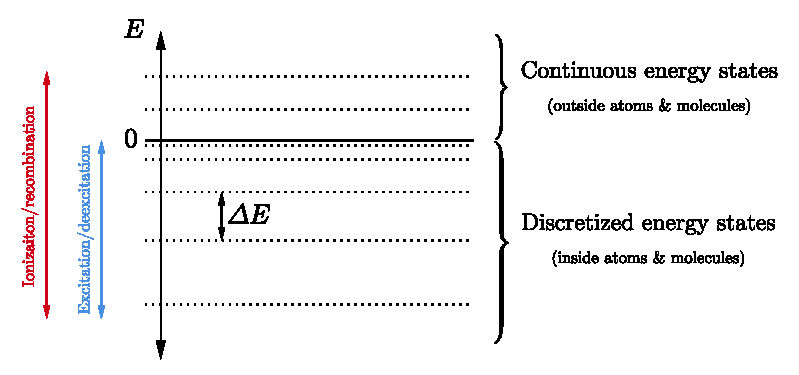
\includegraphics[width=12cm]{figures/energystates.pdf}
\caption{Illustration of discretized and continuous energy states in matter. Note, that the dotted lines for negative energies represent possible energy states within an atom or molecule (bound states), whereas there is actually a continuum of dotted lines for positive energies.}
\label{fig:energylevels}
\end{figure}

Consider now \cref{fig:spectrallineformation}.
\begin{figure}[h]
\centering
\includegraphics[width=10cm]{figures/spectrallineformation.pdf}
\caption{Illustration of a spectral line formation using the Eddington-Barbier relation as an explanatory tool. Note, that in this picture one assumes, that the extinction coefficient $\alpha_\lambda$ is independent of depth $z$, and furthermore, that the source function $S_\lambda = S$ is independent of wavelength and furthermore linear in $z$. This means, that the Eddington-Barbier relation does not only hold approximatively, but exactly. Furthermore, the optical depth is then just given as $\tau_\lambda^\prime(Z) = \int_{0}^{Z}\alpha_\lambda\,\mathrm{d}z = \alpha_\lambda Z$. Figure inspired by \cite[p.38]{Rutten.2015}.}
\label{fig:spectrallineformation}
\end{figure}
Consider a hypothetical atom, which is such that it contains only one electron and which has only two distinct energy states available to the electron. These energy states are separated by the energy $\Delta E$ corresponding to the wavelength $\lambda_\gamma = hc/\Delta E$. Assume further, that there is some hypothetical medium consisting of only those hypothetical atoms along with a electromagnetic radiation source; and that scattering is negligible. At precisely the wavelength $\lambda_\gamma$, this hypothetical medium will perfectly absorb all photons, as long as there are still some energy state changes available. This is to say, that there will also be some spike in the curve of $\alpha_\lambda$, the extinction coefficient, as it is shown in the top left panel of \cref{fig:spectrallineformation} - a spectral line is formed. Now, as such, the spectral line will be just a delta function; in reality however different broadening mechanisms such as Doppler or Lorentz broadening of spectral lines apply, furthermore there are many more than just two energy levels available to electrons in a real medium. Therefore, in \cref{fig:spectrallineformation} the extinction coefficient $\alpha_\lambda$ is plotted for some arbitrary, non-hypothetical medium. One can see, that the absorption line is centered as $\lambda_2$. Assuming, that the extinction coefficient is not dependent upon height $z$ and taking into account the definition of the optical depth $\tau_\lambda^\prime(Z) = \int_{0}^{Z}\alpha_\lambda \,\mathrm{d}z$, one deduces $\tau_{\lambda_1}^\prime(z) = \alpha_{\lambda_1}z$ and $\tau_{\lambda_2}^\prime(z) = \alpha_{\lambda_2}z$. Since $\alpha_{\lambda_1} \gg \alpha_{\lambda_2}$ clearly $\tau_{\lambda_1}^\prime$ must be a steeper function of $z$ than $\tau_{\lambda_2}^\prime$. This is to say, that the medium is more opaque at wavelength $\lambda_2$ than at wavelength $\lambda_1$. Taking into account now the Eddington-Barbier relation, which states, that the source function $S_\lambda$ at optical depth $\tau_\lambda^\prime= 1$ is equal to the outward spectral radiance $I_\lambda^+(0)$ one arrives at a spectral line in emission for an observer measuring $I_\lambda^+(0)$. If however, $\alpha_\lambda$ would have a spike upwards, the spectral line would appear in absorption for an observer at $\tau_\lambda^\prime = 0$.
%Use Eddington-Barbier relation to show that a spike in the extinction coefficient $\alpha_\lambda$ for some wavelength $\lambda$ where emission or absorption happens due to a dominant transition in the considered material leads to a spike in spectral radiance. See slides on spectral line formation and scripts of Rutten.
A study of spectral line properties and an analysis, which parameters and how they influence spectral line formation can lead to insights about the medium, in which they form. Using the theory of radiative transfer and especially simplified atmospheric models of stars for example, one can infer physical properties of an atmosphere, simply by investigating one or more spectral lines formed in the atmosphere under consideration.
% See script of Rutten, solar spectrum formation

\section{Polarimetry}
The subject of polarimetry deals with the polarization properties of electromagnetic waves and how they are affected by the properties of the media they are propagating in. In particular, the presence of a magnetic field in the propagating medium of electromagnetic waves leads to the so-called Zeeman splitting of spectral lines, from which the presence and magnitude of a magnetic field can be deduced. Polarimetry furthermore links observable quantities like the Stokes parameters to the parameters of spectral lines, thus providing insight to the medium, where those spectral lines formed. In the context of stellar atmospheres, polarimetry provides the link between the observable Stokes parameters and the parameters defining the stellar atmosphere, such as the magnetic field strength, inclination and azimuth.
% See slides and book of Landi

\subsection{Zeeman effect}
The Zeeman effect for strong external magnetic fields allows inference about the external magnetic field strength. The presence of such an external magnetic field leads to the splitting of energy levels in atoms and molecules. This is to say, that also one spectral line splits into several spectral lines. According to \cite[p.123]{delToroIniesta.2003}, the Zeeman wavelength splitting $\lambda_B$ can be quantified by means of \begin{equation}\label{eq:zeeman}
\lambda_B = \frac{\lambda^2 \nu_L}{c}, \quad \nu_L = \frac{e|\vect{B}|}{4\pi m c},
\end{equation} where $\nu_L$ is the Larmor frequency, $e$ is the elementary charge, $m$ is the particle mass, $\lambda$ is the wavelength of a spectral line in an inertial frame and $\vect{B}$ is the external magnetic field giving rise to the Zeeman splitting. These formulae can be derived by a rigorous calculation involving perturbation theory in quantum mechanics.
% See slides and book of Landi, possibly also del Toro Iniesta section 8.3 or Griffiths.

\subsection{The Stokes parameters and Stokes vector}
Consider a monochromatic electromagnetic wave $\vect{E}$. In general, $\vect{E}$ is a function of position $\vect{r} \in \mathbb{R}^3$ in euclidean space and time $t$, such that $\vect{E} = \vect{E}(\vect{r},t)$. Without loss of generality, the propagation direction of the monochromatic electromagnetic wave can be defined in $z$-direction, hence \cite[p.121]{Stix.2002} gives a monochromatic wave or arbitrary polarization state as \begin{equation}\label{eq:E-wave}
\vect{E}(\vect{r},t) = \begin{pmatrix}
E_x \cos(k z - \omega t) \\ E_y \cos(kz-\omega t + \xi) \\ 0
\end{pmatrix}, \qquad k = \frac{2\pi}{\lambda}.
\end{equation} The quantity $\xi$ is the phase difference between the amplitude of the electromagnetic wave in $x$-direction and $y$-direction, which together with $E_x$ and $E_y$ therefore accounts for the polarization state of the wave. As a side note, notice that the dispersion relation $\omega = \omega(k)$ for a wave propagating in vacuum can be given as $\omega(k) = 2\pi\nu = ck$. For the above specified electromagnetic wave, the Stokes parameters are defined as \begin{equation}
\vect{I} = \begin{pmatrix}
I \\ Q \\ U \\ V
\end{pmatrix} = \begin{pmatrix}
E_x^2 + E_y^2 \\ E_x^2 - E_y^2 \\ 2E_xE_y\cos(\xi) \\ 2E_xE_y\sin(\xi)
\end{pmatrix},
\end{equation} as given in \cite[p.121]{Stix.2002}. Hereby, the identity $I^2 = Q^2 + U^2 + V^2$ holds, as it is shown by the calculation \begin{align}
\begin{aligned}
Q^2 + U^2 + V^2 &= E_x^4 - 2E_x^2E_y^2 + E_y^4 + 4E_x^2E_y^2\left[\cos^2(\xi) + \sin^2(\xi)\right] \\
&= E_x^4 + 2E_x^2E_y^2 + E_y^4 = (E_x^2+E_y^2)^2 = I^2.
\end{aligned}
\end{align} Since these parameters were defined for a monochromatic electromagnetic wave, the Stokes parameters are in general functions of wavelength; the wavelength dependency of $\vect{I} = \vect{I}(\lambda)$ shall henceforth be indicated by the subscript $\lambda$, such that the Stokes parameters are denoted by \begin{equation}
\vect{I}(\lambda) = \vect{I}_\lambda = (I_\lambda, Q_\lambda, U_\lambda, V_\lambda)^\top,
\end{equation} which is called the Stokes vector, whereby also $I_\lambda^2 = Q_\lambda^2 + U_\lambda^2 + V_\lambda^2$ holds. In \cref{fig:stokesvector}, a schematic representation of the definition of the Stokes parameters (vector) is given. Stokes $Q_\lambda$ and $U_\lambda$ are a measure of linear polarization, while Stokes $V_\lambda$ accounts for the amount of circular polarization present in the electromagnetic waves under consideration.
\begin{figure}[h]
\centering
\includegraphics[width=4.5cm]{figures/stokesvector.pdf}
\caption{Schematic representation of the general Stokes vector $\vect{I}_\lambda$ containing the Stokes parameters $I_\lambda$, $Q_\lambda$, $U_\lambda$ and $V_\lambda$. The observer is looking into negative $z$-direction with respect to the electromagnetic wave as defined by \cref{eq:E-wave}. Figure inspired by \cite[p.17]{DeglInnocenti.2005}.}
\label{fig:stokesvector}
\end{figure}

\subsection{The generalized radiative transfer equation}
In the preceding material, the radiative transfer equation was already derived and solved for the spectral radiance $I_\lambda(\tau_\lambda^\prime, \theta)$ as a function of the continuum optical depth $\tau_\lambda^\prime$ and local inclination $\theta$ of an electromagnetic radiation ray. This radiative transfer equation was given by \begin{equation}
\cos(\theta)\frac{\mathrm{d}I_\lambda(\tau_\lambda^\prime)}{\mathrm{d}\tau_\lambda^\prime} = I_\lambda(\tau_\lambda^\prime)-S_\lambda(\tau_\lambda^\prime).
\end{equation} This equation can be generalized to account not only for changes of the spectral radiance (intensity) $I_\lambda$, but for changes of every Stokes parameter $\vect{I}_\lambda = (I_\lambda, Q_\lambda, U_\lambda, V_\lambda)^\top$. This can be done by means of introducing a propagation matrix $\matr{K}_\lambda(\tau_\lambda^\prime) = \mathds{1} + \matr{N}_\lambda(\tau_\lambda^\prime)$, where $\matr{N}_\lambda(\tau_\lambda^\prime)$ accounts for extinction and emission properties of the medium giving rise to spectral line formation; and where $\mathds{1}$ is the unity matrix. Using the wavelength-dependent propagation matrix $\matr{K}_\lambda$, the generalized radiative transfer equation for the Stokes vector can be written as \begin{equation}\label{eq:generalizedradtransfereq}
\frac{\mathrm{d}\vect{I}_\lambda(\tau_\lambda^\prime)}{\mathrm{d}\tau_\lambda^\prime} = \matr{K}_\lambda(\tau_\lambda^\prime)\left[\vect{I}_\lambda(\tau_\lambda^\prime)-\vect{S}_\lambda(\tau_\lambda^\prime)\right],
\end{equation} as given by \cite[p.150]{delToroIniesta.2003}. Note that the factor of $\cos(\theta)$ is absorbed into the propagation matrix $\matr{K}_\lambda$ in the above equation. In the above formulation of the generalized radiative transfer equation also the source function $S_\lambda(\tau_\lambda^\prime)$ was generalized to the source function vector $\vect{S}_\lambda(\tau_\lambda^\prime) = S_\lambda(\tau_\lambda^\prime)(1,0,0,0)^\top$. It is evident from this form of the equation, that the unity matrix $\mathds{1}$ of the propagation matrix takes care of the extinction and emission in the continuum, while the matrix $\matr{N}_\lambda$ takes into account extinction and emission pertaining to spectral lines. 
% Sections 7.6 & 7.7 in del Toro Iniesta

\subsubsection{Formal solution of the generalized radiative transfer equation}
In order to derive a formal solution to the generalized radiative transfer equation following the treatment in \cite[pp.152-157]{delToroIniesta.2003}, the parameter $\kappa \doteq \tau_\lambda^\prime$ shall be introduced to temporarily simplify the notation, hence yielding the generalized radiative transfer equation to be \begin{equation}\label{eq:generalizedradtransferkappa}
\frac{\mathrm{d}\vect{I}_\lambda(\kappa)}{\mathrm{d}\kappa} = \matr{K}_\lambda(\kappa)\left[\vect{I}_\lambda(\kappa)-\vect{S}_\lambda(\kappa)\right].
\end{equation} Consider now for the moment only the homogeneous differential equation \begin{equation}\label{eq:homogeneralizedradeq}
\frac{\mathrm{d}\vect{I}_{\lambda,h}(\kappa)}{\mathrm{d}\kappa} = \matr{K}_\lambda(\kappa)\vect{I}_{\lambda,h}(\kappa).
\end{equation} As it is done in \cite[p.152]{delToroIniesta.2003}, a so-called evolution operator $\matr{P}(\kappa, \kappa^\prime)$ can be defined, such that it gives the transformation $\vect{I}_{\lambda,h}(\kappa^\prime)\rightarrow \vect{I}_{\lambda,h}(\kappa)$ of the solution $\vect{I}_{\lambda,h}(\kappa^\prime)$ to the homogeneous equation from position $\kappa^\prime$ to $\kappa$, i.e. \begin{equation}\label{eq:evoloperatordef}
\vect{I}_{\lambda,h}(\kappa) = \matr{P}(\kappa,\kappa^\prime)\vect{I}_{\lambda,h}(\kappa^\prime).
\end{equation} This operator is linear, because the differential equation governing $\vect{I}_{\lambda,h}(\kappa)$ is also linear. Furthermore, because of the way it was defined, it has the properties \begin{gather}
\matr{P}(\kappa,\kappa) = \mathds{1}, \qquad \matr{P}(\kappa,\kappa^\prime)\matr{P}(\kappa^\prime, \kappa^{\prime\prime}) = \matr{P}(\kappa,\kappa^{\prime\prime}). 
\end{gather} Differentiating \cref{eq:evoloperatordef} with respect to $\kappa$, namely \begin{align}
\begin{aligned}
\frac{\mathrm{d}\vect{I}_{\lambda,h}(\kappa)}{\mathrm{d}\kappa} = \frac{\mathrm{d}\matr{P}(\kappa,\kappa^\prime)}{\mathrm{d}\kappa}\vect{I}_{\lambda,h}(\kappa^\prime) = \matr{K}_\lambda(\kappa)\matr{P}(\kappa,\kappa^\prime)\vect{I}_{\lambda,h}(\kappa^\prime),
\end{aligned}
\end{align} the identity \begin{equation}\label{eq:grte_op_id_1}
\frac{\mathrm{d}\matr{P}(\kappa,\kappa^\prime)}{\mathrm{d}\kappa} = \matr{K}_\lambda(\kappa)\matr{P}(\kappa,\kappa^\prime)
\end{equation} results. Furthermore differentiating \cref{eq:evoloperatordef} with respect to $\kappa^\prime$ yields \begin{align}
\begin{aligned}
\frac{\mathrm{d}\vect{I}_{\lambda,h}(\kappa)}{\mathrm{d}\kappa^\prime} = \matr{P}(\kappa,\kappa^\prime)\frac{\mathrm{d}\vect{I}_{\lambda,h}(\kappa^\prime)}{\mathrm{d}\kappa^\prime} + \frac{\mathrm{d}\matr{P}(\kappa,\kappa^\prime)}{\mathrm{d}\kappa^\prime}\vect{I}_{\lambda,h}(\kappa^\prime) = 0.
\end{aligned}
\end{align} By means of rearranging this equation and inserting the definition of the homogeneous equation \eqref{eq:homogeneralizedradeq} the equation \begin{align}
\begin{aligned}
\frac{\mathrm{d}\matr{P}(\kappa,\kappa^\prime)}{\mathrm{d}\kappa^\prime}\vect{I}_{\lambda,h}(\kappa^\prime) &= -\matr{P}(\kappa,\kappa^\prime)\frac{\mathrm{d}\vect{I}_{\lambda,h}(\kappa^\prime)}{\mathrm{d}\kappa^\prime} \\ &= -\matr{P}(\kappa,\kappa^\prime)\matr{K}_\lambda(\kappa^\prime)\vect{I}_{\lambda,h}(\kappa^\prime)
\end{aligned}
\end{align} obtains, wherefrom the identity \begin{equation}\label{eq:grte_op_id_2}
\frac{\mathrm{d}\matr{P}(\kappa,\kappa^\prime)}{\mathrm{d}\kappa^\prime} = -\matr{P}(\kappa,\kappa^\prime)\matr{K}_\lambda(\kappa^\prime)
\end{equation} is deduced.

Now, the generalized radiative transfer equation \cref{eq:generalizedradtransferkappa} is multiplied with the operator $\matr{P}(\kappa^\prime, \kappa)$ from the left, thus obtaining \begin{align}
\begin{aligned}
\matr{P}(\kappa^\prime,\kappa)\frac{\mathrm{d}\vect{I}_\lambda(\kappa)}{\mathrm{d}\kappa} &= \matr{P}(\kappa^\prime,\kappa)\matr{K}_\lambda(\kappa)\left[\vect{I}_\lambda(\kappa)-\vect{S}_\lambda(\kappa)\right] \\
&= \frac{\mathrm{d}}{\mathrm{d}\kappa}\left[\matr{P}(\kappa^\prime,\kappa)\vect{I}_\lambda(\kappa)\right] - \frac{\mathrm{d}\matr{P}(\kappa^\prime,\kappa)}{\mathrm{d}\kappa}\vect{I}_\lambda(\kappa) \\
&= -\frac{\mathrm{d}\matr{P}(\kappa^\prime,\kappa)}{\mathrm{d}\kappa}\left[\vect{I}_\lambda(\kappa)-\vect{S}_\lambda(\kappa)\right],
\end{aligned}
\end{align} where the identity \cref{eq:grte_op_id_2} was employed in the last step. Rearranging the above equation yields \begin{align}
\begin{aligned}
\frac{\mathrm{d}}{\mathrm{d}\kappa}\left[\matr{P}(\kappa^\prime,\kappa)\vect{I}_\lambda(\kappa)\right] = \frac{\mathrm{d}\matr{P}(\kappa^\prime,\kappa)}{\mathrm{d}\kappa}\vect{S}_\lambda(\kappa) = -\matr{P}(\kappa^\prime,\kappa)\matr{K}_\lambda(\kappa)\vect{S}_\lambda(\kappa),
\end{aligned}
\end{align} where again identity \cref{eq:grte_op_id_2} was made use of. One has now an integratable equation with respect to $\kappa$. Integrating the left hand side of the above equation from $\kappa_0$ to $\kappa_1$ gives \begin{align}
\begin{aligned}
\int_{\kappa_0}^{\kappa_1}\frac{\mathrm{d}}{\mathrm{d}\kappa}\left[\matr{P}(\kappa^\prime,\kappa)\vect{I}_\lambda(\kappa)\right]\,\mathrm{d}\kappa &= \matr{P}(\kappa^\prime,\kappa_1)\vect{I}_\lambda(\kappa_1) - \matr{P}(\kappa^\prime,\kappa_0)\vect{I}_\lambda(\kappa_0) \\
&= -\int_{\kappa_0}^{\kappa_1}\matr{P}(\kappa^\prime,\kappa)\matr{K}_\lambda(\kappa)\vect{S}_\lambda(\kappa)\,\mathrm{d}\kappa.
\end{aligned}
\end{align} Through rearrangement of the equation and multiplication with $\matr{P}(\kappa_1,\kappa^\prime)$, the expressions \begin{align}
\begin{aligned}
\matr{P}(\kappa_1,\kappa^\prime)\matr{P}(\kappa^\prime,\kappa_1)\vect{I}_\lambda(\kappa_1) &= \matr{P}(\kappa_1,\kappa^\prime)\matr{P}(\kappa^\prime,\kappa_0)\vect{I}_\lambda(\kappa_0) \\
&\quad - \int_{\kappa_0}^{\kappa_1}\matr{P}(\kappa_1,\kappa^\prime)\matr{P}(\kappa^\prime,\kappa)\matr{K}_\lambda(\kappa)\vect{S}_\lambda(\kappa)\,\mathrm{d}\kappa,
\end{aligned}
\end{align} results, which can due to $\matr{P}(\kappa,\kappa^\prime)\matr{P}(\kappa^\prime,\kappa) = \matr{P}(\kappa,\kappa) = \mathds{1}$ and $\matr{P}(\kappa^{\prime\prime},\kappa^\prime)\matr{P}(\kappa^\prime,\kappa) = \matr{P}(\kappa^{\prime\prime},\kappa)$ further simplified to a first formal solution to the generalized radiative transfer equation, namely \begin{equation}
\vect{I}_\lambda(\kappa_1) = \matr{P}(\kappa_1,\kappa_0)\vect{I}_\lambda(\kappa_0)- \int_{\kappa_0}^{\kappa_1}\matr{P}(\kappa_1,\kappa)\matr{K}_\lambda(\kappa)\vect{S}_\lambda(\kappa)\,\mathrm{d}\kappa.
\end{equation} Resubstituting $\tau_\lambda^\prime = \kappa$ and hence $\mathrm{d}\kappa = \mathrm{d}\tau_\lambda^\prime$ and identifying $\kappa_0 = \tau_{\lambda,0}^\prime \rightarrow \infty$ and $\kappa_1 = \tau_{\lambda,1}^\prime\rightarrow \tau_\lambda^\prime$, one gets the general formal solution \begin{align}\begin{aligned}\label{eq:general_sol_gen_rad_transf_eq}
\vect{I}_\lambda(\tau_\lambda^\prime) = \matr{P}\left(\tau_\lambda^\prime,\infty\right)\vect{I}_\lambda(\infty)  -\int_{\infty}^{\tau_\lambda^\prime}\matr{P}\left(\tau_\lambda^\prime,t\right)\matr{K}_\lambda(t)\vect{S}_\lambda(t)\,\mathrm{d}t
\end{aligned}\end{align} to the generalized radiative transfer equation. Considering \cref{fig:outward-inward-radiation}, the optical depth $\tau_\lambda^\prime \rightarrow \infty$ can be understood to be located at the limit, where no photon can ever escape, e.g. at the center of a star, whose radiative transfer is described by \cref{eq:general_sol_gen_rad_transf_eq}. Further taking a closer look at \cref{fig:outward-inward-radiation}, the optical depth $\tau_\lambda^\prime = 0$ can be understood as the position of an observer located outside or right at boundary of the radiative transfer system, that is for example the position of an observer looking at a stellar atmosphere from outside the atmosphere. In this case, the measurable Stokes vector at the position of an observer outside the radiative transfer system is given as \begin{align}\begin{aligned}\label{eq:special_sol_gen_rad_transf_eq}
\vect{I}_\lambda(\tau_\lambda^\prime = 0) = \int_{0}^{ \infty}\matr{P}\left(0,t\right)\matr{K}_\lambda(t)\vect{S}_\lambda(t)\,\mathrm{d}t.
\end{aligned}\end{align} This result is obtained from \cref{eq:general_sol_gen_rad_transf_eq}, where \cite[p.153]{delToroIniesta.2003} gives the limit of the evolution operator $\matr{P}(0,t)$ for $t\rightarrow \infty$ to be \begin{equation}
\lim_{t\rightarrow \infty} \matr{P}(0,t) = 0.
\end{equation} This result makes sense insofar, as this limit can be represented as $\vect{I}_{\lambda,h}(0) = \matr{P}(0,\infty)\vect{I}_{\lambda,h}(\infty)$ by means of using the definition \cref{eq:evoloperatordef} of the evolution operator; it should account for the change in $\vect{I}_{\lambda,h}$ from $\tau_\lambda^\prime \rightarrow \infty$ to $\tau_\lambda^\prime = 0$. Since the solution $\vect{I}_{\lambda,h}$ to the homogeneous radiative transfer equation \cref{eq:homogeneralizedradeq} does not contain any source term, the homogeneous solution must change to zero as one goes from optical depth infinity to optical depth zero. This is because in this case, a ray travels a theoretically infinite distance through the radiative transfer system without any sources along the way, therefore extincting all photons on the way to optical depth zero.
% Section 9.2 in del Toro Iniesta

\subsection{Absorption, emission and dispersion profile functions}
Absorption can be defined as the removal of energy from an electromagnetic field by interaction with matter \cite[p.87]{delToroIniesta.2003}. Emission however, is the opposite of absorption, namely contribution of energy to an electromagnetic field by means of photons emerging from electronic transitions in atoms and molecules. There is a third effect due to the interaction of matter with electromagnetic fields, namely dispersion; \cite[p.87]{delToroIniesta.2003} defines it as the dephasing of the electric field components as the radiation propagates through matter.

Spectral lines due to absorption and emission properties of matter can be accounted for by so-called profile functions. These functions are not just delta functions, as the discrete energy levels in atoms and molecules would suggest, but are always broadened by different processes. Among these processes are the so-called pressure broadening (Lorentz broadening) and the thermal broadening (Doppler broadening). Doppler broadening is caused by the thermal velocities of atoms and molecules in matter, which move in arbitrary directions in general. These effects are accounted for by distinct profile functions; these two profile functions can however be combined to account for both pressure and thermal broadening by means of the mathematical operation of a convolution; thus yielding the Voigt profile function $H(u,a)$ as \begin{equation}\label{eq:Voigt_Profile}
H(u,a) = \frac{a}{\pi}\int_{-\infty}^{\infty}e^{-y^2}\frac{1}{(u-y)^2+ a^2}\,\mathrm{d}y, \end{equation} as given by \cite[p.100]{delToroIniesta.2003}. Furthermore, the dispersion effects are accounted for by the Faraday-Voigt function $F(u,a)$ given by \begin{equation}\label{eq:Faraday_Voigt_Profile}
F(u,a) = \frac{1}{\pi}\int_{-\infty}^{\infty}e^{-y^2}\frac{u-y}{(u-y)^2+a^2}\,\mathrm{d}y.
\end{equation} The Voigt and the Faraday-Voigt profile functions are visualized in \cref{fig:profilefunctions}.
\begin{figure}[h]
\centering
\begin{subfigure}[t]{0.49\textwidth}
    \centering
    \includegraphics[width=\textwidth]{figures/voightprofile.pdf}
    \caption{Voigt profile function for $a=1$.}
    \label{fig:voightprofile}
\end{subfigure}
\hfill
\begin{subfigure}[t]{0.49\textwidth}
    \centering
    \includegraphics[width=\textwidth]{figures/voightfaradayprofile.pdf}
    \caption{Faraday-Voigt profile function for $a=1$.}
    \label{fig:faradayvoightprofile}
\end{subfigure}
\caption{Voigt and Faraday-Voigt profile functions for $a=1$.}
\label{fig:profilefunctions}
\end{figure}

\subsection{The propagation matrix}\label{sec:propagationmatrix}
The propagation matrix $\matr{K}_\lambda(\tau_\lambda^\prime)$ accounts for absorption and dispersion effects of electromagnetic waves in matter within the framework of the generalized radiative transfer equation. In particular, it accounts for spectral lines in a radiation continuum. Explicitly, \cite[p.154]{Stix.2002} gives the propagation matrix to be defined as \begin{equation}
\matr{K}_\lambda = \begin{pmatrix}
\eta_I & \eta_Q & \eta_U & \eta_V \\
\eta_Q & \eta_I & \rho_V & -\rho_U \\
\eta_U & -\rho_V & \eta_I & \rho_Q \\
\eta_V & \rho_U & -\rho_Q & \eta_I
\end{pmatrix}.
\end{equation} The individual entries of this matrix \cite[p.116]{delToroIniesta.2003} accounts for by \begin{align}\begin{aligned}
\eta_I &= 1 + \frac{\eta_0}{2}\left[\phi_0\sin^2(\theta) + \frac{1}{2}(\phi_{+1}+\phi_{-1})(1+\cos^2(\theta))\right], \\
\eta_Q &= \frac{\eta_0}{2}\left[\phi_0-\frac{1}{2}(\phi_{+1}+\phi_{-1})\right]\sin^2(\theta)\cos(2\varphi), \\
\eta_U &= \frac{\eta_0}{2}\left[\phi_0 - \frac{1}{2}(\phi_{+1}+\phi_{-1})\right]\sin^2(\theta)\sin(2\varphi), \\
\eta_V &= \frac{\eta_0}{2}(\phi_{-1}-\phi_{+1})\cos(\theta), \\
\rho_Q &= \frac{\eta_0}{2}\left[\psi_0-\frac{1}{2}(\psi_{+1}+\psi_{-1})\right]\sin^2(\theta)\cos(2\varphi), \\
\rho_U &= \frac{\eta_0}{2}\left[\psi_0-\frac{1}{2}(\psi_{+1}+\psi_{-1})\right]\sin^2(\theta)\sin(2\varphi), \\
\rho_V &= \frac{\eta_0}{2}(\psi_{-1}-\psi_{+1})\cos(\theta).
\end{aligned}
\end{align} Hereby, the angles $\theta$ and $\varphi$ are called inclination and azimuth and are defined as seen in \cref{fig:inclinationazimuth}. \begin{figure}[h]
\centering
\includegraphics[width=8cm]{figures/inclinationazimuth.pdf}
\caption{Visualization of the definitions for the inclination and azimuth angles $\theta$ and $\varphi$.}
\label{fig:inclinationazimuth}
\end{figure} The ranges for those angles are $\theta \in [0,\pi]$ and $\varphi \in [0,\pi]$. In the case of solar observations, $\theta = 0$ means that a vector field $\vect{V}$ under consideration is oriented towards an observer on-looking the Sun, whereas $\varphi=$ does either mean, that the vectorial quantity $\vect{V}$ faces either perfectly west or east on the solar surface. $\theta=\pi$ then does mean, that $\vect{V}$ points exactly away from the observer.

The quantities $\phi_\alpha$ and $\psi_\alpha$ for $\alpha \in \{0,-1,1\}$ are left to be defined; \cite[p.123]{delToroIniesta.2003} defines these parameters as \begin{align}
\begin{aligned}
\phi_\alpha(u,a) &= \frac{1}{\sqrt{\pi}}H(u + \alpha u_B - u_{los}, a), \\
\psi_\alpha(u,a) &= \frac{1}{\sqrt{\pi}}F(u + \alpha u_B - u_{los},a).
\end{aligned}
\end{align} Herewith, $u$, $u_B$ and $u_{los}$ aswell as $a$ are dimensionless quantities determining the the Voigt and Faraday-Voigt functions. In these functions $u$ is related to the wavelength $\lambda$ and is to be regarded as a fixed value for a certain spectral line under consideration. \cite[p.21]{UitenbroekNSME.2020} gives the parameter $u_{los}$ as \begin{equation}
u_{los} = \lambda\frac{\vect{u}\cdot\vect{n}}{c\Delta\lambda_D},
\end{equation} where $\vect{n}$ defines the line of sight vector and $\vect{u}$ the velocity of the medium constituents relative to an inertial observer outside the radiative transfer system. This is a dimensionless number related to the actual line of sight velocity $v_{los}$ as $v_{los} = cu_{los}$. Furthermore, $\Delta \lambda_D$ refers to the Doppler broadening of a spectral line due to the thermal velocity \begin{equation}
v_{th} = \sqrt{\frac{2k_BT}{m}}
\end{equation} of the particles of mass $m$ in the medium; it is given by the expression \begin{equation}
\Delta \lambda_D = \frac{v_{th}\lambda}{c} = \frac{\lambda}{c}\sqrt{\frac{2k_B T}{m}}.
\end{equation} Since the thermal velocity of the particles is responsible for the Doppler broadening, one can also call the thermal velocity $v_{th}$ the Doppler velocity $v_{dop} \doteq v_{th}$. Last but not least, $u_B$ is a factor originating in the Zeeman effect; therefore it connects the radiative transfer equation with an external magnetic field $\vect{B}$ via the relation \begin{equation}
u_B = g_L\frac{e\lambda^2|\vect{B}|}{4\pi m c\Delta \lambda_D},
\end{equation} where $g_L$ is the Landé factor. In total therefore, the propagation matrix $\matr{K}_\lambda$ for a certain wavelength $\lambda$ can be fully determined by means of the seven independent parameters $\{|\vect{B}|, \theta, \varphi, v_{los}, v_{dop}, a, \eta_0\}$.
% Section 7.6 in del Toro Iniesta with
% Profile functions: (6.55)-(6.58).
% Profile functions with Zeeman effect and LOS-velocity: (8.7)-(8.13); (6.42)-(6.48).
% and also picture of azimuth and inclination angles definition with respect to line of sight.

\subsection{The Milne-Eddington approximation}\label{sec:MEapproximation}
% Section 9.4.1 in del Toro Iniesta with eqs. (7.42), (7.43), (7.44), (7.45). 
% Profile functions: (6.55)-(6.58).
% Profile functions with Zeeman effect and LOS-velocity: (8.7)-(8.13); (6.42)-(6.48).
The Milne-Eddington approximation of radiative transfer allows for the construction of a relatively simple stellar atmosphere model $\vect{y} = \vect{M}(\vect{x})$, where $\vect{x}$ would be the atmospheric parameters, such as  magnetic field strength, inclination and so forth, and where $\vect{y}$ would be the predicted observational data, namely the Stokes vectors $\vect{I}_\lambda$ for a certain wavelength interval $\lambda \in [\lambda_-,\lambda_+]$ giving so-called Stokes profiles. A Milne-Eddington model for a stellar atmosphere can even be analytically inverted, which means that there is a mathematically exact way to calculate atmospheric parameters $\vect{x}$ based on observational data $\vect{y}$ by means of mathematically inverting the model, i.e. $\vect{x} = \vect{M}^{-1}(\vect{y})$. In the case of real and not synthetic observational data $\vect{y}$, the best fit to the data given the model $\vect{y} = \vect{M}(\vect{x})$ is to be found by iteratively changing the parameters; that is by means of synthesizing observations, comparing them to the real observations and adjusting the parameters, such that a better fit to the real observations is expected in the next iteration.

The simplest possible solution for the generalized radiative transfer equation \cref{eq:generalizedradtransfereq} is the so-called Milne-Eddington solution. Its derivation relies on the Milne-Eddington approximation, which basically consists of three fundamental assumptions given in \cite[p.411]{DeglInnocenti.2005} profoundly simplifying the radiative transfer problem:
\begin{enumerate}
\item The radiative transfer system is assumed to be of a plane parallel nature and in a local thermal equilibrium.
\item All parameters relevant to spectral line formation are required to be independent of all measures of height within the system.
\item The source function is required to be affinely dependent upon the continuum optical depth.
\end{enumerate}

The second assumption is to say, that the propagation matrix $\matr{K}_\lambda$ is isotropically constant, i.e. \begin{equation}
\matr{K}_\lambda = \matr{K}_{\lambda,0}.
\end{equation} The third ingredient to the Milne-Eddington model means, that the source function vector can be written as \begin{equation}
\vect{S}_\lambda(\tau_\lambda^\prime) = \vect{S}_{\lambda,0} + \tau_\lambda^\prime \vect{S}_{\lambda,1},
\end{equation} where $\vect{S}_{\lambda,0} = S_{\lambda,0}(1,0,0,0)^\top$ and $\vect{S}_{\lambda,1}=S_{\lambda,1}(1,0,0,0)^\top$ are constant vectors. Using the first assumption of the Milne-Eddington model, one can furthermore make the identifications $S_{\lambda,0} = B_\lambda(T)$ and $S_{\lambda,1} = B_\lambda(T)\beta$ with $\beta \in \mathbb{R}$ a constant. This is because local thermal equilibrium implies, that the source function is locally equal to the Planck function.

In the Milne-Eddington case, the homogeneous generalized radiative transfer equation \cref{eq:homogeneralizedradeq} reads as \begin{equation}
\frac{\mathrm{d}\vect{I}_{\lambda,h}(\tau_\lambda^\prime)}{\mathrm{d}\tau_\lambda^\prime} = \matr{K}_{\lambda,0}\vect{I}_{\lambda,h}(\tau_\lambda^\prime).
\end{equation} According to standard mathematical literature, the matrix exponential $e^{\matr{A}}$ for a matrix $\matr{A}$ is defined as \begin{equation}
e^{\matr{A}} = \mathds{1} + \matr{A} + \frac{1}{2!}\matr{A}^2 + \frac{1}{3!}\matr{A}^3 + \dots = \sum_{k=1}^{\infty}\frac{\matr{A}^k}{k!},
\end{equation} Analogously to the scalar case, a solution to the generalized homogeneous radiative transfer equation can be given as \begin{equation}
\vect{I}_\lambda(\tau_\lambda^\prime = 0) = e^{-\matr{K}_{\lambda,0}\tau_\lambda^\prime}\vect{I}_\lambda(\tau_\lambda^\prime).
\end{equation} Comparing this to the definition \cref{eq:evoloperatordef} of the evolution operator, one finds \begin{equation}
\matr{P}(0,\tau_\lambda^\prime) = e^{-\matr{K}_{\lambda,0}\tau_\lambda^\prime}
\end{equation} in the Milne-Eddington case. One can now calculate the solution $\vect{I}_\lambda(\tau_\lambda^\prime=0, \theta)$ using the special case \cref{eq:special_sol_gen_rad_transf_eq} of the formal solution to the generalized radiative transfer equation, namely 
\begin{equation}
\vect{I}_\lambda(\tau_\lambda^\prime = 0,\theta) = \int_{0}^{ \infty}\matr{P}\left(0,t\right)\matr{K}_\lambda(t)\vect{S}_\lambda(t)\,\mathrm{d}t.
\end{equation}
First, note that the derivative of $e^{-\matr{K}_{\lambda,0}\tau_\lambda^\prime}$ is given by \begin{equation}
\frac{\mathrm{d}}{\mathrm{d}\tau_\lambda^\prime}e^{-\matr{K}_{\lambda,0}\tau_\lambda^\prime} = -e^{-\matr{K}_{\lambda,0}\tau_\lambda^\prime}\matr{K}_{\lambda,0},
\end{equation} because \begin{align}
\begin{aligned}
\frac{\mathrm{d}}{\mathrm{d}x}e^{x\matr{A}} &= \frac{\mathrm{d}}{\mathrm{d}x}\left(\mathds{1} + x\matr{A} + \frac{1}{2!}x^2\matr{A}^2 + \frac{1}{3!}x^3\matr{A}^3 + \dots \right) \\
&= \matr{A} + x\matr{A}^2 + \frac{1}{2!}x^2\matr{A}^3 +  \frac{1}{3!}x^3\matr{A}^4 + \dots \\
&= \left(\mathds{1} + x\matr{A} + \frac{1}{2!}x^2\matr{A}^2 +  \frac{1}{3!}x^3\matr{A}^3 + \dots\right)\matr{A} = e^{x\matr{A}}\matr{A},
\end{aligned}
\end{align} hence consequently also $\frac{\mathrm{d}}{\mathrm{d}x}e^{-x\matr{A}} = -e^{x\matr{A}}\matr{A}$ holds for any matrix $\matr{A}$ and real parameter $x$. Therefore, $-e^{-\matr{K}_{\lambda,0}\tau_\lambda^\prime}\matr{K}_{\lambda,0}^{-1}$ is an antiderivative of $-e^{-\matr{K}_{\lambda,0}\tau_\lambda^\prime}$. Now, one proceeds by calculating \begin{align}
\begin{aligned}\label{eq:fundamentalMEsolution}
\vect{I}_\lambda(\tau_\lambda^\prime = 0) &= \int_{0}^{ \infty}\matr{P}\left(0,t\right)\matr{K}_\lambda(t)\vect{S}_\lambda(t)\,\mathrm{d}t \\ &= \int_{0}^{\infty}\underbrace{e^{-\matr{K}_{\lambda,0}t}\matr{K}_{\lambda,0}}_{\doteq\,\tfrac{\mathrm{d}}{\mathrm{d}t}\matr{F}(t)}\underbrace{\left(\vect{S}_{\lambda,0}+t\vect{S}_{\lambda,1}\right)}_{\doteq\,\vect{G}(t)}\,\mathrm{d}t \\
&= \left[\matr{F}(t)\vect{G}(t)\right]^{\infty}_{0} - \int_{0}^{\infty} \matr{F}(t)\frac{\mathrm{d}}{\mathrm{d}t}\vect{G}(t)\,\mathrm{d}t \\
&= \left[-e^{-\matr{K}_{\lambda,0}t}\matr{K}_{\lambda,0}^{-1}\matr{K}_{\lambda,0}(\vect{S}_{\lambda,0}+t\vect{S}_{\lambda,1})\right]^{\infty}_{0} \\ &\quad + \int_{0}^{\infty}e^{-\matr{K}_{\lambda,0}t}\matr{K}_{\lambda,0}^{-1}\matr{K}_{\lambda,0}\vect{S}_{\lambda,1}\,\mathrm{d}t \\
&= \vect{S}_{\lambda,0} + \int_{0}^{\infty}e^{-\matr{K}_{\lambda,0}t}\vect{S}_{\lambda,1}\,\mathrm{d}t \\ &= \vect{S}_{\lambda,0} + \left[e^{-\matr{K}_{\lambda,0}t}\matr{K}_{\lambda,0}^{-1}\vect{S}_{\lambda,1}\right]^{\infty}_0 \\ &= \vect{S}_{\lambda,0}-\matr{K}_{\lambda,0}^{-1}\vect{S}_{\lambda,1}.
\end{aligned}
\end{align} This is the fundamental result of the Milne-Eddington approximation and is sometimes also called the Unno-Rachkovsky solution, as stated by \cite[p.160]{delToroIniesta.2003}. It is important to note here, that $\lambda$ refers to the central wavelength of the considered spectral line(s), which means, that the parameters defining the Milne-Eddington atmosphere are considered to be constant for the wavelength interval(s) around the spectral line(s) under examination. Identifying therefore $\vect{S}_{\lambda,0} = S_{\lambda,0}(1,0,0,0)^\top = S_0(1,0,0,0)^\top$ and $\vect{S}_{\lambda,1} = S_{\lambda,1}(1,0,0,0)^\top = S_1(1,0,0,0)^\top$ and taking into account, that the propagation matrix $\matr{K}_{\lambda,0}$ depends upon the seven parameters as specified in \cref{sec:propagationmatrix}, the Stokes values $\vect{I}_\lambda(\tau_\lambda^\prime =0)$ around the central wavelength $\lambda$ of a spectral line are determined fully by the set  of nine parameters $|\vect{B}|$, $\theta$, $\varphi$, $v_{los}$, $v_{dop}$, $a$, $\eta_0$,   $S_0$, $S_1$. Note, that $S_0$ is related to the Planck function as $B_\lambda(T) = S_0$; therefore, one can also assign a temperature $T$ to the system under investigation once one has a value for $S_0$ and knows which wavelength $\lambda$ to consider.

The parameter vector $\vect{x}$ of the Milne-Eddington model is hence given as \begin{equation}
\vect{x} = (|\vect{B}|,\theta,\varphi,v_{los},v_{dop},a,\eta_0,S_0,S_1)^\top \in \mathbb{R}^9.
\end{equation} 
Let a number $D \in \mathbb{N}$ of wavelengths be sampled from a given wavelength interval $[\lambda_{min},\dots,\lambda,\dots,\lambda_{max}]$ centered around $\lambda$, the central wavelength of a spectral line. Therefore, the observations vector $\vect{y}$ of the Milne-Eddington model is accounted for by \begin{equation}
\vect{y} = (\vect{I}_{\lambda_{min}},\dots,\vect{I}_\lambda,\dots,\vect{I}_{\lambda_{max}})^\top \in \mathbb{R}^D.
\end{equation} 
Thus, the full Milne-Eddington model can be written as \begin{equation}\label{eq:ME_model_equation}
\vect{M}:\mathbb{R}^9 \rightarrow \mathbb{R}^D, \quad \vect{x} = \begin{pmatrix}
|\vect{B}| \\
\theta \\
\varphi \\
v_{los} \\
v_{dop} \\
a \\
\eta_0 \\
S_0 \\
S_1
\end{pmatrix} \mapsto \vect{y} = \vect{M}(\vect{x}) = \begin{pmatrix}
\vect{I}_{\lambda_{min}} \\
\vdots \\
\vect{I}_{\lambda} \\
\vdots \\
\vect{I}_{\lambda_{max}}
\end{pmatrix},
\end{equation}
where \cref{eq:fundamentalMEsolution} is identified to define the model $\vect{y} = \vect{M}(\vect{x})$.

%\subsubsection{Rough implementation of the Milne-Eddington model}
%One can implement a rough Milne-Eddington model  $\vect{y} = \vect{M}(\vect{x})$ as given in \cref{eq:ME_model_equation}. This can be done by means of exactly implementing all equations as specified in \cref{sec:MEapproximation}, e.g. in the programming language \verb|Python|. In \cref{fig:MEroughimplementation}, the results of such a rough implementation can be seen for $u = 2u_{los}$ and the parameter values \begin{gather}\begin{gathered}
%|\vect{B}| = 100.0,\ \theta = \frac{\pi}{2},\ \varphi = \frac{\pi}{2},\ v_{los}=1.0,\ v_{dop}=2.0,\ a = 0.01,\\ \eta_0 = 2.0,\ S_0 = 1.0,\ S_1 = 1.0,\ c = 1.0, \ g_L = 1.0,\ e = 1,\ m=1.
%\end{gathered}\end{gather} As is evident by closer examination, there are some quirks within these plots/results; for example, the stokes $I$ parameter becomes negative at some points, which cannot be true. Likely, these quirks can possibly be explained by numerical issues of the calculations, but further examination of these issues would be needed to either verify or discard this claim.
%\begin{figure}[h]
%\centering
%\includegraphics[width=\textwidth]{figures/MEimplementation.pdf}
%\caption{Rough implementation of the Milne-Eddington model $\vect{y} = \vect{M}(\vect{x})$ as given by \cref{eq:ME_model_equation}. Note, that the plots are given around the central wavelength $\lambda$, of a spectral line, which is set equal to zero in the plots.}
%\label{fig:MEroughimplementation}
%\end{figure}

\section{Stellar atmosphere models}
\subsection{Stellar atmosphere inversions}
Consider some observation $\vect{y}$ of a stellar atmosphere. Assume, that there is a model $\vect{M}$ with associated parameters $\vect{x}$, such that the model is given by the relationship $\vect{M} = \vect{M}(\vect{x}) = \vect{y}$.
% Make a nice graphic for this

So if one knows the parameter values $\vect{x}_0$ of the stellar atmosphere model $\vect{M}$, then observations $\vect{y}_0$ can be generated based on the parameter values $\vect{x}_0$ by means of the relation $\vect{y}_0 = \vect{M}(\vect{x}_0)$; this is called the forward model. However, if one only has observations $\vect{y}_0$ and the stellar model $\vect{M}$, one would like to find out the model parameters $\vect{x}_0$ associated to these observations; this is called the backward model and can be achieved by means of applying the relation $\vect{x}_0 = \vect{M}^{-1}(\vect{y}_0)$. As one can see, this requires a so-called inversion of the atmosphere model $\vect{M}$, which can lead to degeneracy in the model parameters $\vect{x}_0$, meaning that more than one configuration of $\vect{x}_0$ can lead to the same observations $\vect{y}_0$. A normalizing flow helps to disentangle this degeneracy by means of introducing a probability density function for each model parameter, such that the more likely parameter configurations leading to some observations $\vect{y}_0$ can be distinguished from less likely parameter configurations leading to the same observations.

\subsection{Solving a stellar atmosphere inversion problem}
Consider a stellar model $\vect{M}(\vect{x})$. Given observations $\vect{y}_0$, one would like to infer the stellar parameters $\vect{x}_0$ associated to these observations by applying the relation \begin{equation}
\vect{x}_0 = \vect{M}^{-1}(\vect{y}_0).
\end{equation} Commonly, such inversion problems are carried out using a gradient search minimization algorithm which basically functions as follows. First, a function which should be minimized is defined; in our case \begin{equation}
\vect{F}(\vect{x}) \doteq \vect{M}^{-1}(\vect{y}_0) - \vect{x}.
\end{equation} By computing the gradient of $\vect{F}(\vect{x}) = (F_1(\vect{x}), \dots, F_n(\vect{x}))^\top,\,n\in\mathbb{N}$ with respect to the parameters $\vect{x}$, that is for every $F_i \in \vect{F} = (F_1,\dots,F_n)^\top$ the vector $\vect{\nabla}_{\vect{x}}F_i(\vect{x})$ is calculated, one approaches a minimum of $\|\vect{F}\|$, if $\vect{x}$ is iteratively changed in the direction of negative gradient of $\vect{F}(\vect{x})$.

But these types of algorithms are computationally costly, if one wants to infer some sort of distribution of model parameters based on more than just one observation; this is because in the case of multiple observations, as it is almost always the case in real-life applications, a possible solution to the minimization problem needs to be valid for all observations. Furthermore, this procedure just outputs one single vector as a solution. Here the normalizing flows technique comes into play, which provides a computationally more efficient way to do inversions and furthermore allows for the possibility to construct a probability density of possible solutions to the inversion problem, because the a trained normalizing flow outputs not just one single vector as gradient descent does, but a whole bunch of solution vectors. This means, that for each component of these solution vectors one can construct a probability density just by interpolating between the points of a normalized histogram for each component.

\subsection{Calculation of synthesized datasets using a stellar atmosphere model}\label{sec:calcsyntheticdatasets}
In the case, where data $\vect{x} \in \mathbb{R}^d$ is conditioned by context $\vect{y} \in \mathbb{R}^D$, it can be of interest to find a mathematical model implementing a transformation $\vect{y} = \vect{M}(\vect{x})$. In order to be able to train a normalizing flow implementing a transformation \begin{gather}
\vect{f}_{\vect{y},\vect{\phi}(\hat{\matr{x}},\hat{\matr{y}})}: \mathbb{R}^d\rightarrow \mathbb{R}^d, \quad \vect{x}\mapsto \vect{z} =  \vect{f}_{\vect{y},\vect{\phi}(\hat{\matr{x}},\hat{\matr{y}})}(\vect{x}),
\end{gather} if can be a commodity to know the true posterior distribution $p(\vect{x}|\vect{y})$, thus enabling a comparison to the posterior distribution $p_{\vect{\phi}(\hat{\matr{x}},\hat{\matr{y}})}(\vect{x}|\vect{y})$ learned by the normalizing flow; this can be done by application of the Bayes theorem. Note, that $\vect{\phi}(\hat{\matr{x}},\hat{\matr{y}})$ are weights depending upon training data $\hat{\matr{x}}$ and $\hat{\matr{y}}$ associated to the implementation of the function $\vect{f}_{\vect{y},\vect{\phi}}$ by a neural network. As to calculate the true posterior distribution by means of the model $\vect{M}(\vect{x}) = \vect{y}$ linking together the so-called context $\vect{y}$ with the input $\vect{x}$ to the normalizing flow, one can proceed as follows.

First, $\vect{x}$ is assumed to follow a specific probability density $p(\vect{x})$, for example a uniform distribution. Next, one can sample $L\in \mathbb{N}$ datapoints $\{\vect{x}_{1},\dots,\vect{x}_{L}\}$ from the prior $p(\vect{x})$. Using the model $\vect{M}$, for every $\vect{x}_{k}$ the corresponding value $\vect{y}_{k}$ can be calculated as $\vect{y}_{k} = \vect{M}(\vect{x}_{k})$, leading to the likelihood distribution $p(\vect{y}|\vect{x})$. Using the Bayes theorem and the law of total probability, one can calculate $p(\vect{x}_{k}|\vect{y}_{k})$ as \begin{equation}
p(\vect{x}_{k}|\vect{y}_{k}) = \frac{p(\vect{y}_{k}|\vect{x}_{k})p(\vect{x}_{k})}{\sum_{j=1}^{L}p(\vect{y}_{k}|\vect{x}_{j})p(\vect{x}_{j})},
\end{equation} leading to the probability distribution $p(\vect{x}|\vect{y})$ for $k \in \{1,\dots,L\}$ and $L \rightarrow \infty$.

\chapter{Artificial intelligence}
The field of artificial intelligence (AI) is relatively recent field of research dedicated to mimic the process of learning information. Hereby, inspiration for first principles of a sub-field of artificial, the so-called deep learning, comes from the brain structure of mammals. 

As artificial intelligence tries to mimic the process of learning, it remains to be answered what learning actually is. In order to define how a learning process is constituted, another quantity has to be defined first, namely information. \cite[p.2]{Mitchell.1997} defines learning such that a computer program is said to learn from experience $E$ with respect to some class of tasks $T$ and performance measure $P$, if its performance at tasks in $T$, as measured by $P$, improves with experience $E$. If the so-called information entropy, which will be defined at a later stage, serves as a performance measure $P$, the process of learning can also be described by the statement, that any learning process decreases the information entropy of some system under consideration.

\section{Information theory}
Following \cite[p.73]{Goodfellow.2016}, the fundamental intuition of information theory is the consideration, that the occurrence of an unlikely event should convey more information than the occurrence of a likely event. The quantification of information in the field of information theory therefore relies on three key requirements, as given by \cite[p.73]{Goodfellow.2016}:
\begin{enumerate}
\item Likely events should have low information content. Guaranteed events are required to have no information content.
\item Unlikely events should have high information content.
\item Independent events should have additive information; i.e. learning about two independent events of the same likelihood should convey twice as much information as learning about the occurrence of only one of these events.
\end{enumerate} % See deep learning book and lecture

\subsection{Self-information}
The above mentioned requirements are satisfied by the so-called self-information $\mathcal{I}[p(x)]$ as defined by \cite[p.73]{Goodfellow.2016}, namely \begin{equation}\label{eq:defselfinformation}
\mathcal{I}[p(x)] = -\log\left[p(x)\right],
\end{equation} with $X$ being a random variable and $p(x)$ the probability density function thereof.

By this definition, information $\mathcal{I}[p(x=U)]$ of an unlikely event $x=U$ will be higher than information $\mathcal{I}[p(x=L)]$ of a likely event $x = L$; this can be demonstrated by assessing the self-information contents of both events. Because $U$ is said to be an unlikely event, $p(U) \approx 0$ will hold and therefore $\mathcal{I}[p(x=U)] = -\log[p(U)] = \log[1/p(U)] \gg 1$. Since $L$ is a likely event, the probability $p(L)$ of $L$ occurring is estimated by $p(L) \approx 1$ and the self-information $\mathcal{I}[p(x=L)]$ will therefore be very low, because $\mathcal{I}[p(x=L)] = -\log[p(L)] = \log[1/p(L)] \approx 0$ holds. Moreover, information about two independent events $x=A$ and $x=B$ is additive, as the calculation
\begin{align}
\begin{aligned} \mathcal{I}[p(A\cap B)] &= -\log[p(A\cap B)] = -\log[p(A)p(B)] \\ &= -(\log[p(A)] + \log[p(B)]) = \mathcal{I}[p(A)] + \mathcal{I}[p(B)]
\end{aligned}
\end{align} shows it to be the case.

\subsection{Information entropy}
One can describe the information content of a probability density function by the so-called information entropy given by \cite[p.74]{Goodfellow.2016} as
\begin{equation}
H_p[p(x)] = E_{x\sim p}(\mathcal{I}[p(x)]) = -E_{x\sim p}\left(\log[p(x)]\right),
\end{equation} where $p(x)$ is a probability density function of a random variable $X$. If the random variable $X$ is of a discrete nature, the information entropy is called Shannon entropy, whereas if $X$ is continuous, the information entropy goes by the name of differential entropy. % See deep learning book

Information entropy defined in this way is a measure of the amount of uncertainty in a probability distribution. The information entropy will be very low, if $p(x)$ describes mostly very likely events, whereas it will be very high, if $p(x)$ describes mainly very unlikely events. This can also be stated in the following way: Probability distributions that are nearly deterministic (delta-function shaped) have a low entropy, whereas distributions that are closer to a uniform distribution have high entropy.

The field of artificial intelligence and especially its sub-field machine learning are concerned with learning the available self-information from the data. That is to say, the information entropy initially present within the machine learning entity is iteratively reduced by means of training it on a dataset, thus resulting in learned information on the part of the trained artificial intelligence.

\section{Overview of artificial intelligence}
According to \cite[p.7]{Amini.2023}, the field of artificial intelligence can be broadly described as any computational technique, that enables a computer to engage with information in a reasonable way, such as to mimic how a human would process the available data or information. Machine learning is more specialized sub-field of artificial intelligence, which is concerned with any routine, that gives a computer the ability to learn a task without being explicitly programmed for that particular task. Deep learning, which is ultimately about reflecting and rebuilding a simple representation the human brain working principle, is an even more specialized sub-field of artificial intelligence, which is itself a sub-field of machine learning.

The foundational tool of deep learning is the so-called neural network, also known as deep neural network. The basic building block of a neural network is the single layer perceptron (SLP). By combining several single layer perceptrons to a multi layer perceptron (MLP), a deep neural network can be constructed. Given an input vector $\vect{x} = (x_1, \dots, x_d)^\top \in\mathbb{R}^d$ and an output vector $\bar{\vect{x}} = (\bar{x}_1,\dots,\bar{x}_w)^\top \in \mathbb{R}^w$ with $d,w \in \mathbb{N}$, the working principle of single layer perceptron is shown in \cref{fig:SLP}, similarly for a multi layer preceptron in \cref{fig:MLP}.

\section{Neural networks}
% Make analogy to body neuron 
% Parallelize strands with axons, sum with sum of inpulses of axons and activation function with threshold for the neuron to fire
\subsection{Single layer perceptron}
In \cref{fig:SLP}, a single layer perceptron is visualized. The quantity $\vect{x} = (x_1, \dots, x_d)^\top \in\mathbb{R}^d$ with $d \in \mathbb{N}$ is an arbitrary input vector. The single layer perceptron generates a single output $\bar{x}$. First, all input vector components $x_i$ are multiplied with initially arbitrary weights $\phi_i \in \mathbb{R}$ for all $i \in \{1,\dots,d\}$ and subsequently summed up to some sum $\tilde{s} = \sum_{i=1}^{d}x_i\phi_i$; then, an arbitrary bias value $b \in \mathbb{R}$ is added to the sum $\tilde{s}$ such as to arrive at a new sum $s = b + \tilde{s}$. Finally, an output scalar $\bar{x} = a(s)$ is generated by means of pushing the beforehand attained sum $s$ through a so-called activation function $a:\mathbb{R}\rightarrow \mathbb{R}, s\mapsto a(x)$, which is nothing more than some arbitrary nonlinear function, which introduces nonlinearities to the otherwise linear operations; this enables the perceptron to learn nonlinear correlations.
\begin{figure}[h!]
\centering
\includegraphics[width=8cm]{figures/SLP.pdf}
\caption{Working principle of a single layer perceptron; hereby, $a$ represents a nonlinear activation function $a :\mathbb{R}\rightarrow \mathbb{R},\, s\mapsto a(s)$.}
\label{fig:SLP}
\end{figure}
All quantities involving the letters $b$ and $\phi$ compose the total vector $\vect{\phi}$ of weights for the perceptron.

\subsection{Multi layer perceptron}
A multi layer perceptron is the simplest form of a neural network. In \cref{fig:MLP}, such a multi layer perceptron is visualized. Again, $\vect{x} = (x_1, \dots, x_d)^\top$ as an element of $\mathbb{R}^d$ with $d \in \mathbb{N}$ is an arbitrary input vector. Compared to the single layer perceptron, the multi layer perceptron however generates a vectorial output $\bar{\vect{x}} = (\bar{x}_1,\dots,\bar{x}_w)^\top \in \mathbb{R}^w$ with $w \in \mathbb{N}$. Now, all input components $x_i$ are connected to more than one perceptron; thus all perceptrons directly connected to the input components compose a so-called network layer, the first layer. There can be one or more network layers; generally there are $n\in \mathbb{N}$ layers in a neural network. At each perceptron of a certain fixed network layer, a single output is generated as with the single layer perceptron. All of these single outputs together compose a new vector, which serves as the input vector for the next network layer composed of perceptrons. This general working principle is better explained visually, consider therefore \cref{fig:MLP}.
\begin{figure}[h!]
\centering
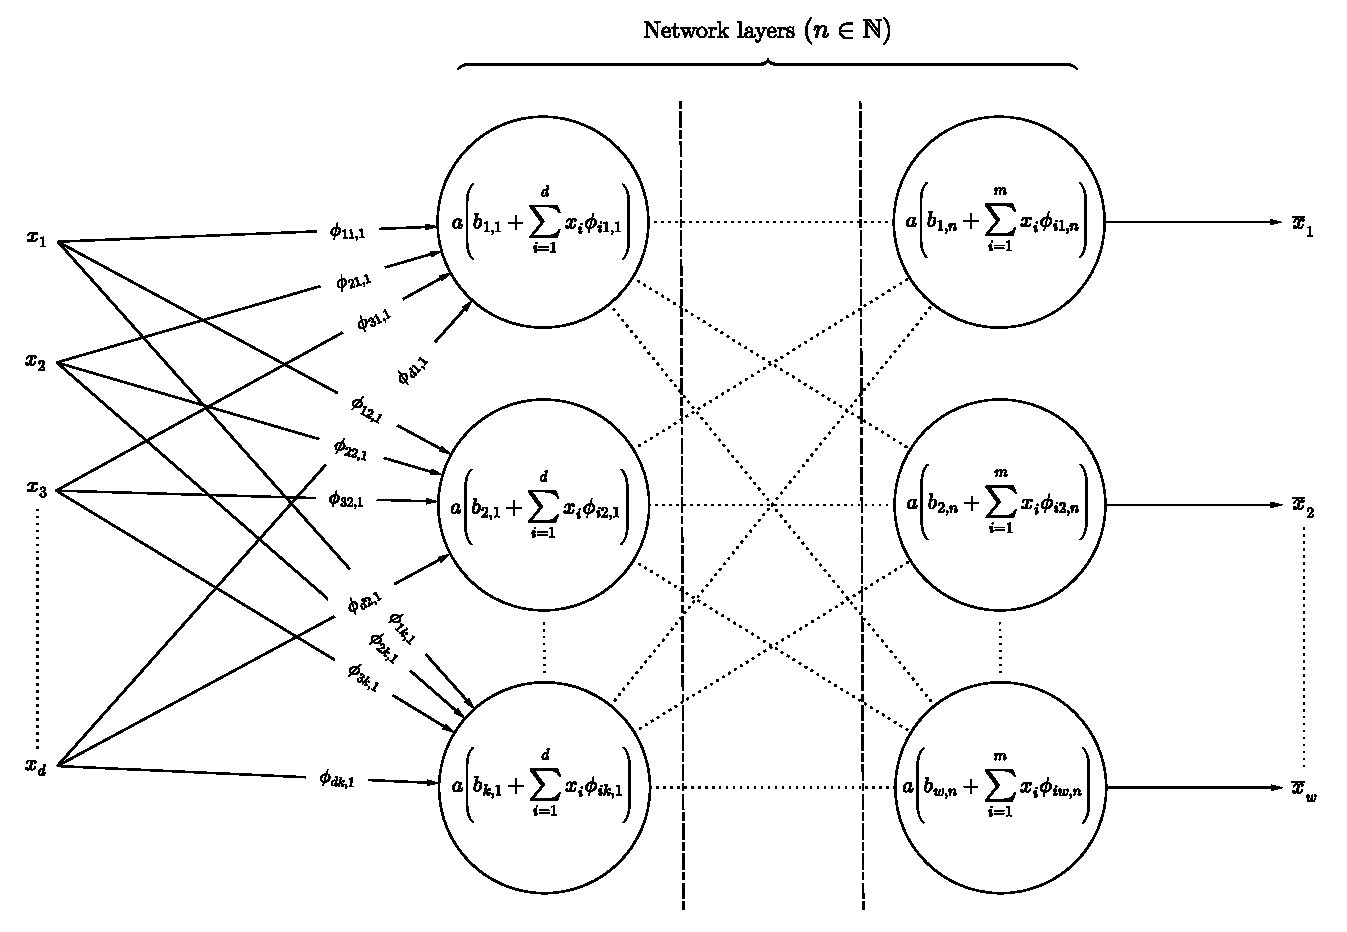
\includegraphics[width=\textwidth]{figures/MLP.pdf}
\caption{Working principle of a multi layer perceptron; hereby, $a$ represents a nonlinear activation function $a :\mathbb{R}\rightarrow \mathbb{R},\, s\mapsto a(s)$.}
\label{fig:MLP}
\end{figure}
Again, all quantities with letters $b$ or $\phi$ compose the total weights vector $\vect{\phi}$ of the multi layer perceptron, which is the simplest possible neural network involving more than one perceptron.

\subsection{Training process for neural networks}
In order for a neural network to learn anything, it has to be conditioned by data, whose interpretation is known. This process is generally referred to as training of a neural network and requires a mathematical framework that allows for optimization. During the training process of a neural network, one would like to achieve the best possible performance of the neural network in interpreting the training data correctly, that is to say, that the input data $\vect{x}$ maps to the known output data $\bar{\vect{x}}$ with minimal discrepancies.

The mathematical framework for such an optimization relies on the definition of a loss function $\mathcal{L}_{\vect{\phi}}$. Such a loss function can be implemented in many different ways; for example on can just take the norm of the difference between input data $\vect{x}$ and output data $\bar{\vect{x}}$ as a loss function, i.e. $\mathcal{L}_{\vect{\phi}(\hat{\matr{x}})} = \|\vect{x}-\bar{\vect{x}}\|$, where $\hat{\matr{x}}$ is a matrix of training data and $\vect{\phi}(\hat{\matr{x}})$ the associated weights of the neural network described by this loss function. However, the loss function depends on the task at hand and needs to be chosen accordingly, such that it represents a suitable measure on how well a neural network learns from the training data. Once one has defined a loss function $\mathcal{L}_{\vect{\phi}}$, the key to training a neural network resides within something called gradient descent. The idea behind gradient descent is quite simple; one just calculates the gradient of the loss function $\mathcal{L}_{\vect{\phi}}$ with respect to the weights $\vect{\phi}$, i.e. $\vect{\nabla}_{\vect{\phi}}\mathcal{L}_{\vect{\phi}}$ and updates all weights such that one moves into the direction of negative gradient. Iteratively repeating this process, eventually a local or global minimum of the loss function is found. In terms of mathematics, this procedure translates as follows. Consider some starting point $\vect{\phi}_i$ and the loss function at this point, i.e. $\mathcal{L}_{\vect{\phi}_i}$. The gradient $\vect{\nabla}\mathcal{L}_{\vect{\phi}}$ of the loss function with respect to the weights $\vect{\phi}$ indicates, in which direction of $\vect{\phi}$ the loss function increases or decreases. The negative gradient points into the direction of a local/global minimum of $\mathcal{L}_{\vect{\phi}}$, whereas the positive gradient points towards a local/global maximum. Hence, $\vect{\phi}_{i+1} = \vect{\phi}_{i} - \gamma \vect{\nabla}_{\vect{\phi}}\mathcal{L}_{\vect{\phi}_i}$ with $i \in \mathbb{N}$ and $\gamma \in \mathbb{R}$ a suitable step size provides a rule for eventually finding a global or local minimum of the loss function. 
\begin{figure}[h]
\centering
\includegraphics[width=7cm]{figures/gradientdescent.pdf}
\caption{Visualization of a gradient descent routine. Note, that the horizontal axis is in reality multidimensional, whereas it is pictured here as just being one-dimensional. The vertical axis represents the value of the loss function $\mathcal{L}_{\vect{\phi}}$ in dependence of the weights $\vect{\phi}$.}
\label{fig:gradientdescent}
\end{figure}
One can therefore define an iterative procedure as follows:
\begin{enumerate}
\item Take a start value $\vect{\phi}_0$ and calculate the value of the loss function $\mathcal{L}_{\vect{\phi}_0}$ at this point.
\item Update the weights $\vect{\phi}_{i}$ according to the rule \begin{equation}
\vect{\phi}_{i+1} = \vect{\phi}_{i} - \gamma \vect{\nabla}_{\vect{\phi}}\mathcal{L}_{\vect{\phi}_i}
\end{equation} for $i \in \mathbb{N}$ individual steps and $\gamma \in \mathbb{R}$ a suitable step size as long as $\epsilon \leq |\mathcal{L}_{\vect{\phi}_{i+1}}-\mathcal{L}_{\vect{\phi}_{i}}|$ holds for $\epsilon \in \mathbb{R}$ an accuracy threshold.
\item Terminate, if $\epsilon > |\mathcal{L}_{\vect{\phi}_{i+1}}-\mathcal{L}_{\vect{\phi}_{i}}|$.
\end{enumerate}
This iterative process is found visualized in \cref{fig:gradientdescent}; note, that this is a simplified picture, as the horizontal axis would in reality be multidimensional.

\subsection{Learning curves}\label{sec:learningcurves}
It is the goal of any entity of machine learning to learn from data in such a way, that it enables the machine learning entity to make as accurate as possible predictions on prior unseen data. \cite[p.110]{Goodfellow.2016} speak in this context of generalization, by which they mean the ability of a machine learning model to perform well on previously unobserved data. In order for a machine learning model to do that, it has to learn model parameters and mathematical operations to predict an outcome, given some input. It is crucial to a good performance of a machine learning model on prior unseen data, that the model learns those parameters and mathematical operations such that there is neither overfitting, underfitting or underrepresentation of training and testing data.

Overfitting is the case, where a model has learned too many parameters, such that it performs extremely well on the training data, but increasingly bad on testing data - that is to say, on prior unseen data to the model. The contrary - underfitting - means, that a model has not learned enough parameters to be able to generalize to prior unseen data.

Apart from overfitting, underfitting or underrepresentation issues, one can certainly ask if it matters, which particular model Ansatz one chooses for a particular task. In fact, \cite[p.116]{Goodfellow.2016} note that the so-called no free lunch theorem states, that every machine learning classification algorithm generalized equally well (or bad), if averaged over all possible data generating probability distributions. But this is not to say, that every machine learning algorithm performs equally well or bad on a particular task - this is not the case. Hence, one must choose the most appropriate machine learning model for the task at hand. Most appropriate in this context is to say, that the chosen model should generalize better than any other available model Ansatz.

Once one has chosen a machine learning model for a particular task, the question of how to ensure, that the model is trained on data in such a way, that it generalizes best to prior unobserved data. Methods to take care of this are generally known as regularization, as \cite[p.120]{Goodfellow.2016} explain.

However, besides regularization, tuning the so-called hyperparameters of a machine learning algorithm can improve its generalization properties. Hyperparameters are just settings of the learning algorithm for a machine learning entity. In order to find optimal hyperparameters, one can either do a so-called grid search algorithms can be applied; or one can just inspect the learning curves for different settings of hyperparameters.
\begin{figure}[h]
\centering
\includegraphics[width=\textwidth]{figures/learningcurves.pdf}
\caption{Examples for the four basic cases of non-ideal model performance. Sketches inspired by Jason Brownlee, \url{https://machinelearningmastery.com/learning-curves-for-diagnosing-machine-learning-model-performance/}, accessed on December 18, 2023.}
\label{fig:learningcurves}
\end{figure}

The concepts of underfitting, overfitting or underrepresentation of either training or testing data for the learning process of a machine learning model reflect in the learning curves as sketched in \cref{fig:learningcurves}. 

As underfitting means, that the model has not learned enough parameters to generalize to unseen data, it reflect in a learning curve such that the train loss is notoriously lower than the test loss and that there is an approximately constant gap between the train and test loss curves after several epochs. This situation is shown on the far left panel of \cref{fig:learningcurves}. 

If however the test loss steadily increases as the train loss continuously decreases, it is very likely that there is overfitting in the model; that is to say, that the model has learned too many model parameters, such that it performs very well on the training data, but increasingly worse on the test data. The situation of overfitting is shown in the second from left panel of \cref{fig:learningcurves}. 

Furthermore, there can also be two cases of underrepresentativeness of either the training dataset or the testing dataset, both of which are visualized in the two panels to the right in \cref{fig:learningcurves}. If the training dataset is not representative of the testing dataset and hence generally on prior unseen data, one would expect that the test loss is higher than the train loss. This is indeed the case for an underrepresentative training dataset; additionally, there can be large fluctuations in the learning curves, since the gradient descent algorithm jumps over local or global minima of the loss function more easily, if the training data has \flqq gaps\frqq.\ On the other hand, if the testing dataset is underrepresentative, one would expect that the test loss is notoriously lower than the train loss - because the average performance of a model trained on a diverse and therefore representative amount of data on a smaller, underrepresentative dataset will be better. That again is the case as shown in the far right panel of \cref{fig:learningcurves}, where again fluctuations are to be expected due to the mentioned reason. 

Another factor that can lead to a behaviour a shown in the second to right panel of \cref{fig:learningcurves} is a learning rate, which is chosen to be too high. If the learning rate is set to too large a rate, the gradient descent process optimizing the model parameters can \flqq jump\frqq\ over minima, leading to an oscillatory behaviour of the train and test loss.

An ideal learning curve is shown in \cref{fig:ideallearningcurve}.
\begin{figure}[h]
\centering
\includegraphics[width=6cm]{figures/ideallearningcurve.pdf}
\caption{Example of an ideal learning curve.}
\label{fig:ideallearningcurve}
\end{figure}
It features a continuously decreasing train and test loss, which eventually seem to converge to a constant value after several epochs and where furthermore the gap between the train and test losses is very small. An ideal learning curve indicates, that the hyperparameter setting for a machine learning model is optimal or at least well-chosen.

Analyzing learning curves visually using these tools can lead to finding optimal hyperparameters for machine learning model and especially for neural networks. Inspecting learning curves can also help to identify possible issues concerning the data itself, for example if the data is underrepresentative of the general diversity of data or not.

\section{Deep generative models}
Generative models - as their name already suggests - generate data. These models learn how to do so by extracting defining features of the data they are trained on, such as the data's probability density. Consider a matrix of training data $\hat{\matr{x}}$, where the individual columns follow a probability distribution $\vect{x} \sim p_{\vect{x}}(\vect{x})$. According to \cite[p.593]{Raschka.2022}, a generative model in deep learning is then defined such, that it learns parameters $\vect{\phi}(\hat{\matr{x}})$ to construct a probability density function $p_{\vect{\phi}(\hat{\matr{x}})}(\vect{x}) \approx p_{\vect{x}}(\vect{x})$. This is to say, that one can then draw samples from the learned probability density $p_{\vect{\phi}(\hat{\matr{x}})}(\vect{x})$, which essentially are generated data imitating the training data.

One can distinguish at least three basic architectures of generative models, namely variational autoencoder networks (VAE's), generative adversarial networks (GAN's) and flows. These types of generative models are visualized in \cref{fig:VAE}, \cref{fig:GAN} and \cref{fig:Flow}. The parallelograms used to visualize the working principles of these models represent dimensionality reduction/increase of an input variable compared to an output variable; if the parallelogram narrows towards the output, it means dimensionality reduction, whereas if it broadens towards the output, increase in dimensionality is visualized.
%Explain why in the context of inversions a flow is desirable (probability distribution for solution, rather than one single value, fast sampling due to essentially just a function, etc.). See blog of Lilian Weng.
\subsection{VAE's}
Variational autoencoders work as sketched in \cref{fig:VAE}. A variational autoencoder consists of an encoder and a decoder. The encoder implements a conditional probability distribution $q_{\vect{\phi}}(\vect{z}|\vect{x})$ for a latent variable $\vect{z}$, based on an input variable $\vect{x}$, where $\vect{\phi}$ are the weights of the neural network constituting the encoder. The decoder however models the probability $p_{\vect{\theta}}(\vect{x}|\vect{z})$ of the output variable $\vect{x}$ based on the latent variable $\vect{z}$, where again $\vect{\theta}$ are weights associated to the neural network of the decoder. The variable $\vect{x}$ represents the input variable with probability density $\vect{x} \sim p_{\vect{x}}(\vect{x})$, whereas the variable $\vect{z}$ is a latent variable and is chosen to fit the probability density of a standard normal distribution, i.e. $\vect{z}\sim p_{\vect{z}}(\vect{z}) = \mathcal{N}(0,1)^d$, where $d \in \mathbb{N}$ is the dimension of the latent variable.
\begin{figure}[h!]
\centering
\includegraphics[width=\linewidth-4cm]{figures/VAE.pdf}
\caption{Working principle of a variational autoencoder (VAE). Figure inspired by \cite{weng2018flow}.}
\label{fig:VAE}
\end{figure}

A variational autoencoder is trained in such a way, that the encoder learns how to transform an input $\vect{x}$ such that the output $\bar{\vect{z}}$ follows the chosen latent probability density. Furthermore, the decoder has to learn, how to transform a variable $\vect{z}$ following a standard normal distribution to an output $\bar{\vect{x}}$, such that the output variable follows the probability density of the original input variable $\vect{x}$.

A VAE in principle can be said to learn the most important information from the training data $\hat{\matr{x}}$, as it has to pass this information from the input variable $\vect{x}$ through a low-dimensional bottleneck to $\bar{\vect{z}}$, from which again the original input $\bar{\vect{x}}$ has to be reconstructed as best as possible, such that $\vect{x} \approx \bar{\vect{x}}$. Once the VAE is trained sufficiently, one can just use the decoder to generate outputs $\bar{\vect{x}}$ based on $\vect{z}$ sampled from a multidimensional standard normal distribution.

A VAE could be used for stellar atmosphere inversion purposes, but it has several disadvantages in this regard compared to normalizing flows. First of all, VAE's have to be trained using an evidence lower bound (ELBO), because the exact likelihood of $\vect{x}$ given $\vect{z}$ is not tractable. A normalizing flow however allows for exact likelihood estimation of $\vect{x}$ given $\vect{z}$ because of its architecture. Furthermore, again because of its inherent architecture, a normalizing flow allows to perform exact inversions of data, since it is basically built of invertible functions. This is not the case for VAE's; yes, encoder and decoder are sort of inverse to one another, but it cannot be an exact inversion in the mathematical sense, since the VAE relies on a smaller dimension of the latent variable and the input/output variable.

\subsection{GAN's}
% Explain what happens with a GAN.
Generative adversarial networks function as sketched in \cref{fig:GAN}. A generative adversarial network consists of a generator and a discriminator. The generator is basically implements a function $\bar{\vect{x}} = \vect{G}_{\vect{\phi}}(\vect{z})$, where $\bar{\vect{x}}$ is the output of the generator, $\vect{\phi}$ are the weights associated to the neural network implementing the generator function and $\vect{z}$ is a latent variable, which is chosen to follow a standard normal distribution, i.e. $\vect{z} \sim p_{\vect{z}}(\vect{z}) = \mathcal{N}(0,1)^d$ with $d \in \mathbb{N}$ again the dimensionality of the latent space. The purpose of the generator is to generate fake data $\bar{x}$ based on samples $\vect{z}$ of the latent probability density $p_{\vect{z}}(\vect{z})$. The discriminator however takes an input $\vect{x}$, such as the output of the generator, and outputs a value 0 or 1, where 0 stands for \flqq input is fake\frqq\ and 1 represents the situation \flqq input is real\frqq.\ The task of the discriminator is therefore to decide, if an input $\vect{x}$ is fake or real.
\begin{figure}[h!]
\centering
\includegraphics[width=\linewidth-4cm]{figures/GAN.pdf}
\caption{Working principle of a generative adversarial network (GAN). Figure inspired by \cite{weng2018flow}.}
\label{fig:GAN}
\end{figure}

A generative adversarial network is trained in such a way, that the generator learns how to generate the best possible real-looking data $\bar{\vect{x}}$, whereas the discriminator learns as good as possible to distinguish between real data contained in the training set $\hat{\matr{x}}$ and fake data $\bar{\vect{x}}$ generated by the generator. Herein lies the adversarity of the model; the generator and the discriminator are actually competing against each other; the generator learns how to create the best possible fake data, whereas the discriminator learns, how to best distinguish between real and fake data - in this way, both the generator and the discriminator are optimized for their respective task. The loss function for training therefore has to be defined accordingly in a game-theoretical manner, where both the discriminator and the generator try to optimize their outcomes. Once trained, one can just use the generator to create fake data $\bar{\vect{x}} = \vect{G}_{\vect{\phi}}(\vect{z})$ from samples $\vect{z}$ of $p_{\vect{z}}(\vect{z})$ at will.

Despite the many interesting applications of GAN's, they cannot really be used for stellar atmosphere inversion purposes, since they do not suit the problem at hand, since stellar inversion problems do not involve classification between real and fake data.

\subsection{Flows}
Flow-based generative models work as sketched in \cref{fig:Flow}. A flow just consists of a bijective function $\bar{\vect{z}} = \vect{f}_{\vect{\phi}}(\vect{x})$, where $\vect{\phi}$ refers to the weights of the neural network(s) used to implement this function. One of the main differences between flows and GAN's on the one hand and VAE's on the other hand is the fact, that flows are bijective in architectural nature, while GAN's and VAE's are not. This is to say that they are perfectly adapted to an inversion problem, such as a stellar atmosphere inversion task. Because of the bijective nature of flows, there is no dimensionality reduction or increase from input/output to latent space.
\begin{figure}[h!]
\centering
\includegraphics[width=\linewidth-4cm]{figures/Flow.pdf}
\caption{Working principle of a flow-based generative model. Figure inspired by \cite{weng2018flow}.}
\label{fig:Flow}
\end{figure}

Flows can be trained by exact likelihood calculation; that is to say, the loss function can be mathematically derived and implemented using the change of variable theorem from probability calculus in combination with the specific bijective transformations constituting the flow. A flow is called a normalizing flow, if the latent probability density function is chosen as a standard normal distribution - hence an arbitrary probability density $p_{\vect{x}}(\vect{x})$ of input data is mapped into the density of a standard normal distribution. In that way, the input data can be said to be normalized to the latent space. As flows and especially normalizing flows are best suited to stellar atmosphere inversions compared to the other available generative models, this technique will be the tool of choice in the material to follow.

%\section{Role of CPU's and GPU's in machine learning tasks}
%So-called CPU's (central processing unit) are those hardware components in a computer, which executes most of the computer's hardware and software instructions. CPU's performs tasks sequentially; therefore a CPU can only handle multiple tasks at the same time if there are multiple cores in the CPU.
%
%So-called GPU's (graphics processing unit) are those hardware components in a computer, which render intensive high-resolution graphics or images. GPU's can perform tasks in parallel processing; therefore a GPU can handle multiple tasks at the same time by splitting up a task in multiple sub-tasks and dividing them among the vast number of processing cores in the GPU.
%
%A CPU typically operates much faster than a GPU, but can handle tasks only sequentially. A GPU however typically consists of a vast number of cores allowing for efficient multitasking. In general therefore, a GPU can handle intensive calculations faster than a CPU, because it allows for dividing a task in multiple sub-tasks and distributing them among the vast number of processing cores, whereas the CPU cannot do that but can only handle tasks in a sequential way.
%
%For machine learning therefore, it is often the case that a GPU's are required for time-efficient computing.


%\section{Kullback-Leibler divergence}
%The Kullback-Leibler divergence is a means to compute how different two probability distributions $p(x)$ and $q(x)$ over the same random variable $X$ are. It is defined as \begin{equation}
%D_{KL}(p||q) = E_{x\sim p}\left[\log\left(\frac{p(x)}{q(x)}\right)\right] = E_{x\sim p}\left(\log[p(x)]-\log[q(x)]\right).
%\end{equation} As such, the Kullback-Leibler divergence is nothing more than the difference between a so-called cross-entropy $H_p[q(x)]$ and an entropy $H_p[q(x)]$, namely \begin{gather}\begin{gathered}
%D_{KL}(p||q) = H_p[q(x)]- H_p(p(x)) = -E_{x\sim p}(\log[q(x)]) + E_{x\sim p}(\log[p(x)]) \\ = E_{x\sim p}(\log[p(x)]- \log[q(x)]).
%\end{gathered}\end{gather} The Kullback-Leibler divergence will be low, if $p(x)$ and $q(x)$ are very similar; it will be high, if $p(x)$ and $q(x)$ are very different. 
%
%As information entropy is a measure for uncertainty in a probability distribution, divergence is to be interpreted as additional uncertainty accounting for the distance between two probability distributions over the same random variable. If $p(x)$ is the target probability distribution, i.e. the true distribution for the random variable $X$, and if $q(x)$ is the model probability distribution, i.e. the learned distribution, the Kullback-Leibler divergence provides a measure on how close the model probability distribution $q(x)$ is to the target distribution $p(x)$. Minimizing the Kullback-Leibler divergence is equivalent to finding the best model probability distribution $q(x)$ in terms of optimal resemblance to the target distribution $p(x)$.
\FloatBarrier

\section{Introduction to normalizing flows}
Normalizing flows are useful to learn complex data distributions from available samples, be they experimentally obtained or of a synthesized nature. 

The goal of a normalizing flow is to learn a certain probability density function $p_{\vect{x}}(\vect{x})$ of some quantity represented by a potentially multivariate random variable $\vect{x}$. Given samples from $p_{\vect{x}}(\vect{x})$ obtained by either experimental or synthetical procedure, the normalizing flow can learn the probability density function by means of finding a diffeomorphism, which maps samples $\vect{z}$ from a standard normal distribution to $p_{\vect{x}}(\vect{x})$. Since a diffeomorphism is invertible by definition, a trained normalizing flow can then be used to draw samples from $p_{\vect{x}}(\vect{x})$ at will; this can be done by sampling from a standard normal distribution and subsequent application of the inverse learned diffeomorphism to the generated samples. This will result in a set of samples from $p_{\vect{x}}(\vect{x})$.

This technique can be used for various purposes; for example, for inversion problems in (stellar) atmospheric physics, as it is being explored in the subsequent material.

%The paper ``Bayesian Stokes inversion with normalizing flows'' by Diaz Baso et al. explores the possibility of a normalizing flow applied to learn how to do an inversion of a stellar atmosphere. 
%
%The paper is concerned with a classical inversion problem concerning stellar atmospheres. That is to say, that one would like to infer possible values for parameters of a solar model depending on measurement data. The paper elaborates on a method, called the Bayesian Stokes inversion with normalizing flows, in order to infer a parameter space of a stellar atmosphere model based on observations. What is special about this method is the fact, that not only certain solution values for the model parameters, but a whole distribution of possible solution values for these parameters are obtained.

\subsection{Why use normalizing flows for inversions?}
If one has an analytical model $\vect{y} = \vect{M}(\vect{x})$ of a stellar atmosphere, it can usually be inverted too, such that $\vect{x} = \vect{M}^{-1}(\vect{y})$. This raises the question, why one should even bother using normalizing flows to learn such inversions.

First of all, only simple models of radiative transfer, such as the Milne-Eddington atmosphere can be inverted analytically. More complex models require resource-demanding calculations by means of Monte Carlo methods to do inversions. The advantage of a normalizing flow resides in the fact, that inversions done by it would be comparatively much faster, once the normalizing flow is trained.

A second incentive to use normalizing flow for atmospheric inversions is, that a normalizing flow not only provides one with one solution to the inversion problem for each atmospheric parameter, but rather with a probability distribution for each parameter. This allows for error estimation and the determination of the most likely solution to an inversion problem, if there is more than one solution possible.

\section{Change of variable formula in probability theory}
The change of variable formula can be considered as the heart of the normalizing flow technique, since it guides the implementation of a loss function to train a flow. Because of its importance for normalizing flows, a full proof of this theorem will therefore be given for the univariate case, which will be generalized to the multivariate case subsequently.
\begin{tm}
Let $x$ and $z$ be continuous random variables with associated probability density functions $p_x(x)$ and $p_z(z)$. Furthermore, let $z$ be the transformation of $x$ by an invertible and strictly increasing continuously differentiable function $f(x)$, such that $z=f(x)$ and $x = f^{-1}(z)$ hold; in this case the change of variable formula from probability theory applies as \begin{equation}
p_x(x) = p_z(f(x))\frac{\mathrm{d}f(x)}{\mathrm{d}x}.
\end{equation}
\end{tm}
\begin{proof}
First, let with $a$ and $b$ be defined real numbers with $a<b$. By definition of the transformation $f(x)$ let with $c$ and $d$ be defined the real numbers $c = f(a)$ and $d=f(b)$, hence \begin{equation}
P(a \leq x \leq b) = P(c \leq z \leq d)
\end{equation} must hold, where this quantity is defined as $P(a \leq x \leq b) \doteq \int_a^b p_x(x)\,\mathrm{d}x$ and therefore represents the probability mass for an experiment outcome of $x$ to be between $a$ and $b$. Since $x$ and $z$ are continuous random variables with associated valid probability density functions, one can write \begin{equation}
P(c \leq z \leq d) = \int_c^d p_z(z)\,\mathrm{d}z = \int_{f^(a)}^{f(b)}f_z(z)\,\mathrm{d}z.
\end{equation} By the substitution rule for integrals one can substitute in the above integral $z(x) = f(x)$ and \begin{equation}
\frac{\mathrm{d}z(x)}{\mathrm{d}x} = \frac{\mathrm{d}f(x)}{\mathrm{d}x} \quad \Leftrightarrow \quad \mathrm{d}z=\mathrm{d}z(y) = \frac{\mathrm{d}f(x)}{\mathrm{d}x}\,\mathrm{d}x.
\end{equation} Therefore, the relation \begin{align}\begin{aligned}
P(c \leq z \leq d) &= \int_{f(a)}^{f(b)}p_z(z)\,\mathrm{d}z \\ &= \int_{a}^{b}p_z(f(x))\frac{\mathrm{d}f(x)}{\mathrm{d}x}\,\mathrm{d}x = P(a \leq x \leq b)
\end{aligned}\end{align} obtains, thus
\begin{equation}
p_x(x) = p_z(f(x))\frac{\mathrm{d}f(x)}{\mathrm{d}x}
\end{equation}
must hold, where $\nicefrac{\mathrm{d}f(x)}{\mathrm{d}x}$ acts as a normalizing factor for the new probability density $p_x(x)$.
\end{proof}

Let now $\vect{x}, \vect{z} \,\in\mathbb{R}^d,\,d\in\mathbb{N}$ be continuous multivariate random variables with associated probability density functions $p_{\vect{x}}(\vect{x})$ and $p_{\vect{z}}(\vect{z})$. Furthermore, let 
\begin{equation} 
\vect{f}:\mathbb{R}^d \rightarrow \mathbb{R}^d, \quad \vect{x}\mapsto\vect{z} = \vect{f}(\vect{x}) 
\end{equation} be a diffeomorphism transforming $\vect{x}$ to $\vect{z}$. In this case, the formula generalizes to the multivariate case as \begin{align}\begin{aligned}
p_{\vect{x}}(\vect{x}) &= p_{\vect{z}}[\vect{f}(\vect{x})]\left|\det\left(\frac{\partial \vect{f}(\vect{x})}{\partial \vect{x}}\right)\right| \\ &= p_{\vect{z}}[\vect{f}(\vect{x})]\left|\det\begin{pmatrix}
\tfrac{\partial f_1(\vect{x})}{\partial x_1} & \dots & \tfrac{\partial f_1(\vect{x})}{\partial x_d} \\
\vdots & \ddots & \vdots \\
\tfrac{\partial f_d(\vect{x})}{\partial x_1} & \dots & \tfrac{\partial f_d(\vect{x})}{\partial x_d}
\end{pmatrix}\right|.
\end{aligned}\end{align}

\section{General principle of a normalizing flow}
% See Li Weng blog, just general theory without diving deep into

\subsection{Conceptual formulation of a normalizing flow}
Consider some vector $\vect{x} \in \mathbb{R}^d$ with $d,\,q \in \mathbb{N}$ and a latent vector $\vect{z} \in \mathbb{R}^d$. The probability densities for these vectors shall be given by \begin{equation}
\vect{x} \sim p_{\vect{x}}(\vect{x}), \quad \vect{z}\sim p_{\vect{z}}(\vect{z}) = \mathcal{N}(0,1)^d.
\end{equation}

The aim of a normalizing flow is to learn a diffeomorphism \begin{equation}
\vect{f}_{\vect{\phi}(\hat{\matr{x}})}:\mathbb{R}^d \rightarrow \mathbb{R}^d, \quad \vect{x} \mapsto \vect{z} = \vect{f}_{\vect{\phi}(\hat{\matr{x}})}(\vect{x})
\end{equation} transforming the probability density function $p_{\vect{x}}$ to $p_{\vect{z}}$. The conceptual principle of a normalizing flow is visualized in \cref{fig:normflow}. 
\begin{figure}[h]
\centering
\includegraphics[width=10cm]{figures/normflow.pdf}
\caption{Conceptual principle of a normalizing flow $\vect{z} = \vect{f}_{\vect{\phi}(\hat{\matr{x}})}(\vect{x})$ transforming a target probability density function $p_{\vect{x}}(\vect{x})$ to a base probability density function $p_{\vect{z}}(\vect{z})$.}
\label{fig:normflow}
\end{figure}
Hereby, $\vect{\phi}(\hat{\matr{x}})$ are weights depending on training data $\hat{\matr{x}} \in \mathbb{R}^{d\times q}$, which are associated to a deep neural network implementing the diffeomorphic function $\vect{f}_{\vect{\phi}(\hat{\matr{x}})}$. Given such a function, using the change of variable formula the probability density $p_{\vect{x}}(\vect{x})$ can be calculated as \begin{equation}
p_{\vect{x}}(\vect{x}) = p_{\vect{z}}[\vect{f}_{\vect{\phi}(\hat{\matr{x}})}(\vect{x})]\left|\det\left(\frac{\partial \vect{f}_{\vect{\phi}(\hat{\matr{x}})}(\vect{x})}{\partial \vect{x}}\right)\right|.
\end{equation} Knowing the transformation $\vect{z} = \vect{f}_{\vect{\phi}(\hat{\matr{x}})}(\vect{x})$ and given that $\vect{z} \sim \mathcal{N}(0,1)^d$, one can easily calculate samples from the distribution $p_{\vect{x}}(\vect{x})$ by means of sampling $\vect{z}$ from a $d$-dimensional standard normal distribution and obtaining the corresponding $\vect{x}$ plugging $\vect{z}$ into the inverse function $\vect{f}_{\vect{\phi}(\hat{\matr{x}})}^{-1}$, such that $\vect{x} = \vect{f}_{\vect{\phi}(\hat{\matr{x}})}^{-1}(\vect{z})$.

\subsection{Requirements for a normalizing flow}
Consider a function 
\begin{equation}
\vect{f}:\mathbb{R}^d \rightarrow \mathbb{R}^d, \quad \vect{x} \mapsto \vect{z} = \vect{f}(\vect{x})
\end{equation} composed of several functions $\vect{f}_{(k)}$, $k \in \{1,\dots,n\},\,n \in \mathbb{N}$, such that \begin{equation}
\vect{z} = \vect{f}(\vect{x}) = \vect{f}_{(n)} \circ \dots \circ \vect{f}_{(1)}(\vect{x}).
\end{equation} In this case, the transformation functions $\vect{f}_{(k)}$ aswell as the function $\vect{f}$ as a whole should satisfy several conditions to serve purposefully as a tool to sample from a probability density $p_{\vect{x}}(\vect{x})$ given samples $\vect{z}$ obtained from a standard normal distribution $p_{\vect{z}}(\vect{z})$. According to \cite{Kobyzev.2021}, all functions $\vect{f}_{(k)}$ should satisfy the following conditions:
\begin{enumerate}
\item All transformation functions $\vect{f}_{(k)}$ need to be invertible and differentiable. In order to transform one probability density into another density, it is necessary to calculate the Jacobian of the transformation function, as stated by the change of variable theorem. Furthermore, the transformation functions should be invertible, because one would like to sample from a standard normal distribution, plug the obtained values $\vect{z}$ into the inverse transformation function and thereby obtaining samples $\vect{x}$. Both of these conditions - invertibility and differentiabiliby - are satisfied by diffeomorphic functions.
\item The transformation functions $\vect{f}_{(k)}$ need to be expressive enough to model real data distributions. The normalizing flow composed of these transformation functions needs to learn a real data distribution; hence enough flexibility of the transformation functions is required in order to allow the neural networks composing the flow to learn actual and potentially complicated probability distributions.
\item The transformation functions $\vect{f}_{(k)}$ should be computationally efficient. That is, the Jacobian determinant should be calculable in an as efficient as possible way; furthermore also the application of the trained forward and inverse normalizing flow should consume as little as possible time. In order to train and apply the normalizing flow, i.e. the transformation functions composing the normalizing flow, many Jacobian determinants need to be calculated, as required by the change of variable formula. Therefore, transformation functions with a simple Jacobians allowing for quick and easy calculations of the corresponding determinants are preferable.
\end{enumerate}

\subsection{Normalizing flows with conditioning data}
Consider a model $\vect{M}(\vect{x}) = \vect{y}$, that produces observations $\vect{y} \in \mathbb{R}^D,\,D \in \mathbb{N}$ based on model parameters $\vect{x}\in\mathbb{R}^d,\,d,\,q \in \mathbb{N}$. Furthermore, consider a latent vector $\vect{z} \in \mathbb{R}^d$. The probability densities for these vectors are given by \begin{equation}
\vect{x} \sim p_{\vect{x}}(\vect{x}), \quad \vect{y} \sim p_{\vect{y}}(\vect{y}), \quad \vect{z}\sim p_{\vect{z}}(\vect{z}) = \mathcal{N}(0,1)^d.
\end{equation}

The aim of the normalizing flow is to model the probability density $p_{\vect{\phi}(\hat{\matr{x}},\hat{\matr{y}})}(\vect{x}|\vect{y})$, namely the probability density function of $\vect{x}$, given a certain observation $\vect{y}$, thereby defining an inversion of the model $\vect{M}(\vect{x}) = \vect{y}$, see \cref{fig:normflowconditional} for a visualization of a normalizing flow with conditioning data; which from now on will be called a conditional normalizing flow.
\begin{figure}[h]
\centering
\includegraphics[width=\textwidth]{figures/normflowconditional.pdf}
\caption{Conceptual principle of a conditional normalizing flow $\vect{z} = \vect{f}_{\vect{y},\vect{\phi}(\hat{\matr{x}},\hat{\matr{y}})}(\vect{x})$, transforming a target probability density function $p_{\vect{x}}(\vect{x})$ to a base probability density function $p_{\vect{z}}(\vect{z})$ conditional on $\vect{y} = \vect{M}(\vect{x})$, where $\vect{M}$ is a model that relates the data $\vect{x}$ to the conditioning data $\vect{y}$.}
\label{fig:normflowconditional}
\end{figure}
The multidimensional quantity $\vect{\phi}(\hat{\matr{x}},\hat{\matr{y}})$ is a set of parameters learned by a neural network, which is used to implement the normalizing flow.

If there is no conditioning data $\vect{y}$ available, the normalizing flow can directly be applied to learn the probability distribution $p_{\vect{\phi}(\hat{\matr{x}})}(\vect{x})$ based on standard normally distributed data $z \sim p_{\vect{z}}(\vect{z}) = \mathcal{N}(0,1)^d$. In this case, the conditioning data $\vect{y}$, i.e. the symbols $\vect{y}$ and $\hat{\matr{y}}$, can be omitted in all formulae pertaining to the current chapter of this document.

\subsection{Coupling layer normalizing flows}\label{subsec:couplinglayernormalizingflows}
Consider a diffeomorphism \begin{equation}
\vect{f}_{\vect{y},\vect{\phi}(\hat{\matr{x}},\hat{\matr{y}})}: \mathbb{R}^d \rightarrow \mathbb{R}^d, \quad \vect{x} \mapsto \vect{z} = \vect{f}_{\vect{y},\vect{\phi}(\hat{\matr{x}},\hat{\matr{y}})}(\vect{x}),
\end{equation} where $\vect{\phi}(\hat{\matr{x}},\hat{\matr{y}})$ are weights depending on training data $\hat{\matr{x}} \in \mathbb{R}^{d\times q}$ and $\hat{\matr{y}} \in \mathbb{R}^{D \times q}$, which are associated to a deep neural network implementing the diffeomorphic function $\vect{f}_{\vect{y},\vect{\phi}(\hat{\matr{x}}, \hat{\matr{y}})}$. The probability density for $\vect{x}$ as calculated via $\vect{x}= \vect{f}^{-1}_{\vect{y},\vect{\phi}(\hat{\matr{x}},\hat{\matr{y}})}(\vect{z})$ therefore becomes conditional on the context $\vect{y}$, because the network parameters $\vect{\phi}(\hat{\matr{x}},\hat{\matr{y}})$ themselves depend on the context $\hat{\matr{y}}$ used to train the network. Hence for $p_{\vect{x}}(\vect{x})$, the notation $p_{\vect{x}}(\vect{x}) = p_{\vect{\phi}(\hat{\matr{x}},\hat{\matr{y}})}(\vect{x}|\vect{y})$ is introduced.

With the change of variable theorem, one obtains \begin{align}
\begin{aligned}
1 = \int_{\mathbb{R}^d} p_{\vect{z}}(\vect{z})\,\mathrm{d}\vect{z} &= \int_{\mathbb{R}^d}p_{\vect{z}}[\vect{f}_{\vect{y},\vect{\phi}(\hat{\matr{x}},\hat{\matr{y}})}(\vect{x})]\left|\det\left(\frac{\partial \vect{f}_{\vect{y},\vect{\phi}(\hat{\matr{x}},\hat{\matr{y}})}(\vect{x})}{\partial \vect{x}}\right)\right|\,\mathrm{d}\vect{x} \\ &= \int_{\mathbb{R}^d} p_{\vect{\phi}(\hat{\matr{x}},\hat{\matr{y}})}(\vect{x}|\vect{y})\,\mathrm{d}\vect{x},
\end{aligned}
\end{align} from which it follows, that the probability density $p_{\vect{\phi}(\hat{\matr{x}},\hat{\matr{y}})}(\vect{x}|\vect{y})$ can be expressed by means of the diffeomorphism $\vect{f}_{\vect{y},\vect{\phi}(\hat{\matr{x}},\hat{\matr{y}})}$, the Jacobian $\tfrac{\partial \vect{f}_{\vect{y},\vect{\phi}(\hat{\matr{x}},\hat{\matr{y}})}(\vect{x})}{\partial \vect{x}}$ and the probability density $p_{\vect{z}}(\vect{z})$, namely \begin{equation}\label{eq:heartofnormflowswithcontext}
p_{\vect{\phi}(\hat{\matr{x}},\hat{\matr{y}})}(\vect{x}|\vect{y}) = p_{\vect{z}}[\vect{f}_{\vect{y},\vect{\phi}(\hat{\matr{x}},\hat{\matr{y}})}(\vect{x})]\left|\det\left(\frac{\partial \vect{f}_{\vect{y},\vect{\phi}(\hat{\matr{x}},\hat{\matr{y}})}(\vect{x})}{\partial \vect{x}}\right)\right|.
\end{equation} This identity is to be considered as the key to implementing a loss function for the normalizing flow technique.

Since a concatenation of diffeomorphisms is again a diffeomorphism, the function $\vect{f}_{\vect{y},\vect{\phi}(\hat{\matr{x}},\hat{\matr{y}})}$ can be composed of many diffeomorphisms. Let $\vect{f}_{\vect{y},\vect{\phi},(1)}, \dots, \vect{f}_{\vect{y},\vect{\phi},n}$ with $n \in \mathbb{N}$ be a number of diffeomorphisms, such that \begin{equation}
\vect{f}_{\vect{y},\vect{\phi}(\hat{\matr{x}},\hat{\matr{y}})} = \vect{f}_{\vect{y},\vect{\phi},(n)}\circ \dots \circ \vect{f}_{\vect{y},\vect{\phi},(1)}.
\end{equation} Introducing the notation $\vect{x} \doteq \vect{z}_{(0)}$, $\vect{z} \doteq \vect{z}_{(n)}$ and $\vect{z}_{(k)} \doteq \vect{f}_{\vect{y},\vect{\phi},(k)}(\vect{z}_{(k-1)})$ with $k \in \{1,\dots,n\}$, the function $\vect{f}_{\vect{y},\vect{\phi}(\hat{\matr{x}},\hat{\matr{y}})}$ can be written as \begin{equation}
\vect{f}_{\vect{y},\vect{\phi}(\hat{\matr{x}},\hat{\matr{y}})}(\vect{z}_{(0)}) = \vect{f}_{\vect{y},\vect{\phi},(n)}\circ \dots\circ \vect{f}_{\vect{y},\vect{\phi},(1)}(\vect{z}_{(0)}).
\end{equation} 
In \cref{fig:normflows}, an overview of the working principle of a coupling layer normalizing flow is visualized.
\begin{figure}[h!]
\centering
\includegraphics[width=\textwidth]{figures/normflows.pdf}
\caption{Visualization of the working principle of coupling layer normalizing flows.}
\label{fig:normflows}
\end{figure}
Because $\vect{f}_{\vect{y},\vect{\phi}(\hat{\matr{x}},\hat{\matr{y}})}(\vect{x})$ is a concatenation of functions $\vect{f}_{\vect{y},\vect{\phi},(k)}(\vect{z}_{(k-1)})$ with $k \in \{1,\dots,n\}$, the determinant of the Jacobian  for $\vect{f}_{\vect{y},\vect{\phi}(\hat{\matr{x}},\hat{\matr{y}})}(\vect{x})$ with respect to $\vect{x}$ is given by \begin{equation}
\det\left(\frac{\partial \vect{f}_{\vect{y},\vect{\phi}(\hat{\matr{x}},\hat{\matr{y}})}(\vect{x})}{\partial \vect{x}}\right) = \prod_{k=1}^{n}\det\left(\frac{\partial \vect{f}_{\vect{y},\vect{\phi},(k)}(\vect{z}_{(k-1)})}{\partial \vect{z}_{(k-1)}}\right),
\end{equation} where the Jacobians on the right-hand side take the form \begin{equation}
\frac{\partial \vect{f}_{\vect{y},\vect{\phi},(k)}(\vect{z}_{(k-1)})}{\partial \vect{z}_{(k-1)}} = 
\begin{pmatrix}
\frac{\partial f_{\vect{y},\vect{\phi},(k),1}(\vect{z}_{(k-1)})}{\partial z_{(k-1),1}} & \dots & \frac{\partial f_{\vect{y},\vect{\phi},(k),1}(\vect{z}_{(k-1)})}{\partial z_{(k-1),d}} \\
\vdots & \ddots & \vdots \\
\frac{\partial f_{\vect{y},\vect{\phi},(k),d}(\vect{z}_{(k-1)})}{\partial z_{(k-1),1}} & \dots & \frac{\partial f_{\vect{y},\vect{\phi},(k),d}(\vect{z}_{(k-1)})}{\partial z_{(k-1),d}}
\end{pmatrix}
\end{equation} with $k \in \{1,\dots,n\}$. 
Every function $\vect{f}_{\vect{y},\vect{\phi},(k)}(\vect{z}_{(k-1)})$ for $k \in \{1,\dots,n\}$ represents one of the $n$ so-called coupling layers constituting the total flow function $\vect{f}_{\vect{y},\vect{\phi}(\hat{\matr{x}},\hat{\matr{y}})}$. Every composite function $\vect{f}_{\vect{y},\vect{\phi},(k)}$ is implemented by application of neural networks depending on $\vect{x}$ and $\vect{y}$, such that each composite function is fully invertible and differentiable. The total set of parameters learned by the neural networks is then identified with $\vect{\phi}(\hat{\matr{x}},\hat{\matr{y}})$, hence defining the function $\vect{f}_{\vect{y},\vect{\phi}(\hat{\matr{x}},\hat{\matr{y}})}$.

\section{Affine coupling layer normalizing flow}\label{subsec:normflowsaffinecouplinglayers}
Affine coupling layer normalizing flows\cprotect\footnote{A basic implementation of an affine coupling layer normalizing flow in the \verb|PyTorch| framework, alongside with two example applications, is given by the author at \url{https://github.com/danielzahnd/master-thesis/tree/main/code/nf-affine-coupling-layer-normalizing-flow}. This code can in principle be applied to any other set of data.\label{footnote:NF_code}} are one of the most simple types of normalizing flows. They basically rely on a concatenation of many affine transformations, where the scale and shift parameters are implemented as neural networks. Although quite easy to implement, these type of flows lack flexibility, as noted by \cite[p.3]{Durkan.10.06.2019}. However, they provide good insight to the working principle of a normalizing flow and are sufficiently flexible for some less complex applications as shown in \cref{chap:proofofconcept}.
 
\subsection{Construction of an affine coupling layer normalizing flow}
Consider a diffeomorphism \begin{align}\footnotesize \begin{aligned}
\vect{f}_{\vect{y},\vect{\phi}(\hat{\matr{x}},\hat{\matr{y}})} = \vect{f}_{\vect{y},\vect{\phi},(n)}\circ \dots \circ \vect{f}_{\vect{y},\vect{\phi},(1)}: \mathbb{R}^d \rightarrow \mathbb{R}^d, \quad \vect{x} \mapsto \vect{z} = \vect{f}_{\vect{y},\vect{\phi}(\hat{\matr{x}},\hat{\matr{y}})}(\vect{x}),
\end{aligned}\end{align} where all quantities are given as defined in \cref{subsec:couplinglayernormalizingflows}. 

In the case of $\vect{f}_{\vect{y},\vect{\phi},(k)}$ being so-called affine coupling layers, the functions can explicitly written by means of two arbitrary functions \begin{equation}
\vect{\mu}_{(k)}: \mathbb{R}^{m+D} \rightarrow \mathbb{R}^{d-m}, \quad \vect{\sigma}_{(k)}: \mathbb{R}^{m+D} \rightarrow \mathbb{R}^{d-m}
\end{equation} with $m \in \{1,\dots,d\}$ and $k \in \{1,\dots,n\}$ implemented as deep neural networks. That is to say, that the neural networks $\vect{\mu}_{(k)}$ and $\vect{\sigma}_{(k)}$ take a vector of dimension $m+D$ as an input and return a vector of dimension $d-m$ as an output; there can be an arbitrary sequence of network layers and activation functions in between input and output. Every mapping $\vect{z}_{(k)} = \vect{f}_{\vect{y},\vect{\phi},(k)}(\vect{z}_{(k-1)})$ for $k \in \{1,\dots,n\}$ is now defined as an affine transformation, such that \begin{align}
f_{\vect{y},\vect{\phi},(k),l}(\vect{z}_{(k-1)}) &= z_{(k-1),l}, \\
f_{\vect{y},\vect{\phi},(k-1),l}^{-1}(\vect{z}_{(k)}) &= 
z_{(k),l}
\end{align} for $l \in \{1,\dots,m\}$
and
\begin{align}
f_{\vect{y},\vect{\phi},(k),l}(\vect{z}_{(k-1)}) &= 
\mu_{(k),l}(\vect{z}_{(k-1),1:m},\vect{y}) + e^{\sigma_{(k),l}(\vect{z}_{(k-1),1:m},\vect{y})}\cdot z_{(k-1),l}, \\
f_{\vect{y},\vect{\phi},(k-1),l}^{-1}(\vect{z}_{(k)}) &= [z_{(k),l} - \mu_{(k),l}(\vect{z}_{(k),1:m},\vect{y})]\cdot  e^{-\sigma_{(k),l}(\vect{z}_{(k),1:m},\vect{y})}
\end{align} for $l \in \{m+1,\dots,d\}$, where $\vect{f}_{\vect{y},\vect{\phi},(k)} = (f_{\vect{y},\vect{\phi},(k),1},\dots,f_{\vect{y},\vect{\phi},(k),d})^\top$ and $\vect{z}_{(k),1:m} = (z_{(k),1},\dots, z_{(k),m})^\top$.

It is a convenient property of such affine functions $\vect{f}_{\vect{y},\vect{\phi},(k)}(\vect{z}_{(k-1)})$ for $k \in \{1,\dots,n\}$, that the Jacobians with respect to $\vect{z}_{(k-1)}$ are triangular, that is 
\begin{gather}\footnotesize\begin{gathered}
\frac{\partial \vect{f}_{\vect{y},\vect{\phi},(k)}(\vect{z}_{(k-1)})}{\partial \vect{z}_{(k-1)}} = 
\begin{pmatrix}
\mathds{1}_m & \mathds{O}_m \\
\frac{\partial \vect{f}_{\vect{y},\vect{\phi},(k),m+1:d}(\vect{z}_{(k-1)})}{\partial \vect{z}_{(k-1),m+1:d}} &  \mathrm{diag}\left(e^{\sigma_{(k),m+1:d}(\vect{z}_{(k-1),1:m},\vect{y})}\right)
\end{pmatrix},
\end{gathered}\end{gather} where $\mathds{1}_m$ is a unity matrix and $\mathds{O}_m$ is a zero matrix of dimension $m \times m$. The lower left quantity in the above matrix is again a Jacobian and takes the form \begin{gather}\scriptsize\begin{gathered}
\frac{\partial \vect{f}_{\vect{y},\vect{\phi},(k),m+1:d}(\vect{z}_{(k-1)})}{\partial \vect{z}_{(k-1),m+1:d}} = \begin{pmatrix}
\frac{\partial f_{\vect{y},\vect{\phi},(k),m+1}(\vect{z}_{(k-1)})}{\partial z_{(k-1),m+1}} & \dots & \frac{\partial f_{\vect{y},\vect{\phi},(k),m+1}(\vect{z}_{(k-1)})}{\partial z_{(k-1),d}} \\
\vdots & \ddots & \vdots \\
\frac{\partial f_{\vect{y},\vect{\phi},(k),d}(\vect{z}_{(k-1)})}{\partial z_{(k-1),m+1}} & \dots & \frac{\partial f_{\vect{y},\vect{\phi},(k),d}(\vect{z}_{(k-1)})}{\partial z_{(k-1),d}}
\end{pmatrix};
\end{gathered}\end{gather} the lower right quantity however is a diagonal matrix with the elements $e^{\sigma_{(k),l}(\vect{z}_{(k-1),1:m},\vect{y})}$ for $l \in \{m+1,d\}$ on the diagonal. Therefore, the Jacobian $\nicefrac{\partial \vect{f}_{\vect{y},\vect{\phi},(k)}(\vect{z}_{(k-1)})}{\partial \vect{z}_{(k-1)}}$ is triangular and hence its determinant is given by the product of the diagonal elements, that is \begin{equation}
\det\left(\frac{\partial \vect{f}_{\vect{y},\vect{\phi},(k)}(\vect{z}_{(k-1)})}{\partial \vect{z}_{(k-1)}}\right) = \prod_{j = m+1}^{d}e^{\sigma_{(k),j}(\vect{z}_{(k-1),1:m},\vect{y})}.
\end{equation} Taking the logarithm of this expression results in a transformation of the product to a sum, such that \begin{equation}\label{eq:previouslogdetc}
\log\left[\det\left(\frac{\partial \vect{f}_{\vect{y},\vect{\phi},(k)}(\vect{z}_{(k-1)})}{\partial \vect{z}_{(k-1)}}\right)\right] = \sum_{j = m+1}^{d}\sigma_{(k),j}(\vect{z}_{(k-1),1:m},\vect{y})
\end{equation} holds. Recall, that the complete normalizing flow is given as a concatenation of affine coupling functions (layers), such that \begin{gather}
\begin{gathered}
\det\left(\frac{\partial \vect{f}_{\vect{y},\vect{\phi}(\hat{\matr{x}},\hat{\matr{y}})}(\vect{x})}{\partial \vect{x}}\right) = \prod_{k = 1}^{n}\det\left(\frac{\partial \vect{f}_{\vect{y},\vect{\phi},(k)}(\vect{z}_{(k-1)})}{\partial \vect{z}_{(k-1)}}\right).
\end{gathered}
\end{gather} Taking the logarithm of this expression and inserting the previous result \cref{eq:previouslogdetc}, this  leads to \begin{align}\label{eq:finallogdetaffinecouplingc}
\begin{aligned}
\log\left[\det\left(\frac{\partial \vect{f}_{\vect{y},\vect{\phi}(\hat{\matr{x}},\hat{\matr{y}})}(\vect{x})}{\partial \vect{x}}\right)\right] &= \sum_{k = 1}^{n}\log\left[\det\left(\frac{\partial \vect{f}_{\vect{y},\vect{\phi},(k)}(\vect{z}_{(k-1)})}{\partial \vect{z}_{(k-1)}}\right)\right] \\
&= \sum_{k = 1}^{n}\sum_{j = m+1}^{d}\sigma_{(k),j}(\vect{z}_{(k-1),1:m},\vect{y}).
\end{aligned}
\end{align}

\subsection{Training process for affine coupling layer normalizing flows}
Recalling the diffeomorphism $\vect{z} = \vect{f}_{\vect{y},\vect{\phi}(\hat{\matr{x}},\hat{\matr{y}})}(\vect{x})$ and the change of variable formula for the multivariate case, the probability density $p_{\vect{\phi}(\hat{\matr{x}},\hat{\matr{y}})}(\vect{x}|\vect{y})$ can be written as found in \cref{eq:heartofnormflowswithcontext}. Taking the natural logarithm of expression \cref{eq:heartofnormflowswithcontext} and inserting the result \cref{eq:finallogdetaffinecouplingc} into it, one obtains
\begin{align}\begin{aligned}
\log\left[p_{\vect{\phi}(\hat{\matr{x}},\hat{\matr{y}})}(\vect{x}|\vect{y})\right] &= \log\left(p_{\vect{z}}[\vect{f}_{\vect{y},\vect{\phi}(\hat{\matr{x}},\hat{\matr{y}})}(\vect{x})]\right) \\ &\quad + \left|\sum_{k = 1}^{n}\sum_{j = m+1}^{d}\sigma_{(k),j}(\vect{z}_{(k-1),1:m},\vect{y})\right|.
\end{aligned}\end{align} Note, that the natural logarithm $\log(a)$ is strictly monotonic increasing for $a > 0$; furthermore, $-\infty < \log(a) \leq 0$ for $ 0 < a \leq 1$. Therefore, maximizing the so-called likelihood $p_{\vect{\phi}(\hat{\matr{x}},\hat{\matr{y}})}(\vect{x}|\vect{y})$ is equivalent to maximizing $\log\left[p_{\vect{\phi}(\hat{\matr{x}},\hat{\matr{y}})}(\vect{x}|\vect{y})\right]$, which is named the log-likelihood. Maximizing $p_{\vect{\phi}(\hat{\matr{x}},\hat{\matr{y}})}(\vect{x}|\vect{y})$ corresponds to finding optimal network parameters $\vect{\phi}(\hat{\matr{x}},\hat{\matr{y}})$ for the deep neural networks $\vect{\mu}_{(k)}$ and $\vect{\sigma}_{(k)}$ for $k \in\{1,\dots,n\}$ constituting the flow function $\vect{f}_{\vect{y},\vect{\phi}(\hat{\matr{x}},\hat{\matr{y}})}$, such that the most suitable model parameters $\vect{x}$ given some context $\vect{y}$ are found. In the case of a stellar atmosphere inversion, $p_{\vect{\phi}(\hat{\matr{x}},\hat{\matr{y}})}(\vect{x}|\vect{y})$ represents a probability distribution for the solutions $\vect{x}$ of an inversion $\vect{x} = \vect{M}^{-1}(\vect{y})$, where $\vect{M}$ is the atmosphere model and $\vect{y}$ are observations.

That is to say, that the normalizing flow, i.e. the neural networks constituting it, are trained by means of minimizing the negative log-likelihood $-\log\left[p_{\vect{\phi}(\hat{\matr{x}},\hat{\matr{y}})}(\vect{x}|\vect{y})\right]$, which is equivalent to maximizing positive log-likelihood and hence also to maximizing the positive likelihood. Therefore, the loss function to minimize by any gradient-descent and backpropagation algorithm employed can be defined as 
\begin{align}\footnotesize
\begin{aligned}
\mathcal{L}_{\vect{\phi}(\hat{\matr{x}},\hat{\matr{y}})}(\vect{x},\vect{y}) =&  -\log\left(p_{\vect{z}}[\vect{f}_{\vect{y},\vect{\phi}(\hat{\matr{x}},\hat{\matr{y}})}(\vect{x})]\right) - \log\left(\left|\det\left(\frac{\partial \vect{f}_{\vect{y},\vect{\phi}(\hat{\matr{x}},\hat{\matr{y}})}(\vect{x})}{\partial \vect{x}}\right)\right|\right) \\
=& -\log\left(p_{\vect{z}}[\vect{f}_{\vect{y},\vect{\phi}(\hat{\matr{x}},\hat{\matr{y}})}(\vect{x})]\right) - \left|\sum_{k = 1}^{n}\sum_{j = m+1}^{d}\sigma_{(k),j}(\vect{z}_{(k-1),1:m},\vect{y})\right|.
\end{aligned}
\end{align} This loss function is minimized with respect to the neural network parameters $\vect{\phi}(\hat{\matr{x}},\hat{\matr{y}})$.


%\section{Autoregressive normalizing flow}\label{subsec:normflowsautoregressive}
%\subsection{Conceptual formulation and terminology}
%Text.
%
%\subsection{Construction of an autoregressive normalizing flow}
%Text.
%
%\subsection{Training process for autoregressive normalizing flows}
%Text.

\section{Piecewise rational quadratic spline normalizing flow}\label{subsec:normflowspiecewiserational}
Affine coupling layer normalizing flows as describe in detail above are simple and relatively easy to implement, but they lack flexibility. As \cite[p.3]{Durkan.10.06.2019} note, affine coupling layer flows may struggle to model especially multimodal density functions using just affine transformations. Recall, that as a base density, usually a standard normal distribution is taken. If there are now multiple modes present in the target distribution of the data to model, the flow needs to learn how to transform just one mode present in the base distribution to the multiple modes in the multimodal target distribution, thus presenting the flow with the need to learn potentially highly nonlinear transformation. This is where affine coupling layer normalizing flows are at their limit.

Hence, \cite[p.4]{Durkan.10.06.2019} introduce piecewise rational quadratic spline normalizing flows, which are more flexible in nature, but mathematically still relatively simple and furthermore fully invertible and differentiable, thus diffeomorphic.

This type of normalizing flow is therefore the flow of choice for the more complex applications as presented and discussed in \cref{chap:results_and_discussion}. These kind of flows were however not implemented from scratch by the author, but the already existing software \cite{nflows} was made use of; and the theoretical considerations below follow the material as presented by \cite{Durkan.10.06.2019}.

\subsection{Construction of a piecewise rational quadratic spline normalizing flow}\label{sec:piecewisequadraticspline}
Consider a diffeomorphism \begin{align}\small\begin{aligned}
\vect{f}_{\vect{y},\vect{\phi}(\hat{\matr{x}},\hat{\matr{y}})} = \vect{f}_{\vect{y},\vect{\phi},(n)}\circ \dots \circ \vect{f}_{\vect{y},\vect{\phi},(1)}: \mathbb{R}^d \rightarrow \mathbb{R}^d, \quad \vect{x} \mapsto \vect{z} = \vect{f}_{\vect{y},\vect{\phi}(\hat{\matr{x}},\hat{\matr{y}})}(\vect{x}).
\end{aligned}\end{align} In the case of this function being implemented by piecewise rational quadratic spline coupling layers, these individual layers can be defined as follows.

Again, $\vect{x} \sim p_{\vect{x}}(\vect{x})$ and $\vect{y} \sim p_{\vect{y}}(\vect{y})$ hold, whereas the modelled probability density of $\vect{x}$ conditional on $\vect{y}$ as learned by a normalizing flow is denoted as $\vect{x} \sim p_{\vect{\phi}(\hat{\matr{x}},\hat{\matr{y}})}(\vect{x}|\vect{y})$, where $\vect{\phi}(\hat{\matr{x}},\hat{\matr{y}})$ are weights associated to the neural network(s) used to implement the flow. The quantities $\hat{\matr{x}} \in \mathbb{R}^{d\times q}$ and $\hat{\matr{y}} \in \mathbb{R}^{D \times q}$ are just training data.

Consider an input vector $\vect{x} \in \mathbb{R}^d$ and a conditioning vector $\vect{y} \in \mathbb{R}^D$. Let now be a vector $\vect{s}$ defined, such that it contains the first $m$ entries of the input vector $\vect{x}$ and the whole conditioning vector $\vect{y}$, that is to say, $\vect{s} \doteq (x_1,\dots,x_m,y_1,\dots,y_D) \in \mathbb{R}^{m+D}$. In order to define a single layer $f_{\vect{y},\vect{\phi},(k)}$ with $k \in \{1,\dots,n\}$ of the flow, one requires $(d-m)(3K-1)$ parameters per layer $k$ These parameters are given for each layer $k$ by means of a neural network \begin{equation}
\vect{\mu}_{(k)}: \mathbb{R}^{m+D}\rightarrow \mathbb{R}^{(d-m)(3K-1)}, \quad \vect{s}_{(k-1)} \mapsto \vect{\phi}_{(k)} = \vect{\mu}_{(k)}(\vect{s}_{(k-1)})
\end{equation} whereby $m \in \{1,\dots,d\}$, $k \in \{1,\dots,n\}$ and $K \in \mathbb{N}$. The integer $K$ is the number of spline knots of choice. The precise nature of the mapping $\vect{\mu}_{(k)}$ is that of an arbitrary neural network, which therefore cannot be explicitly written, but can be accounted for by
\begin{align}
\begin{aligned}
\vect{\phi}_{(k)} = \vect{\mu}_{(k)}(\vect{s}_{(k-1)}) = \begin{pmatrix}
\phi_{(k),m+1,1}^w \\
\vdots \\
\phi_{(k),i,j}^w \\
\vdots \\
\phi_{(k),d,K}^w \\
\phi_{(k),m+1,1}^h \\
\vdots \\
\phi_{(k),i,j}^h \\
\vdots \\
\phi_{(k),d,K}^h \\
\phi_{(k),m+1,1}^\delta \\
\vdots \\
\phi_{(k),i,j}^\delta \\
\vdots \\
\phi_{(k),d,K-1}^\delta \\
\end{pmatrix} \in \mathbb{R}^{(d-m)(3K-1)}
\end{aligned}
\end{align}
in the general case. Let furthermore $\vect{\phi}_{(k),(i)}$ with $i \in \{m+1,\dots,d\}$ be defined as \begin{align}\small\begin{aligned}
\vect{\phi}_{(k),(i)} \doteq (\phi_{(k),i,1}^w,\dots,\phi_{(k),i,K}^w, \phi_{(k),i,1}^h, \dots, \phi_{(k),i,K}^h, \phi_{(k),i,1}^\delta, \dots,\phi_{(k),i,K-1}^\delta)^\top.
\end{aligned}\end{align} The letter $w$ denotes the with of bins, $h$ the height of bins and $\delta$ the derivatives at the internal points.

The last ingredients to be finally able to define the individual transformations $\vect{f}_{\vect{y},\vect{\phi},(k)}$ are $d-m$ actual quadratic functions \begin{equation}
g_{\vect{\phi}_{(k),(i)}} : \mathbb{R} \rightarrow \mathbb{R}
\end{equation} for each coupling layer $k$. Now, each coupling layer $k$ is defined as \begin{equation}
\vect{f}_{\vect{y},\vect{\phi},(k)} : \mathbb{R}^d \rightarrow \mathbb{R}^d, \quad \vect{z}_{(k-1)} \mapsto \vect{z}_{(k)} = \begin{pmatrix}
z_{(k-1),1} \\
\vdots \\
z_{(k-1),m} \\
g_{\vect{\phi}_{(k),(m+1)}}(z_{(k-1),m+1}) \\
\vdots \\
g_{\vect{\phi}_{(k),(d)}}(z_{(k-1),d})
\end{pmatrix},
\end{equation} where $\vect{x} = \vect{z}_{(0)}$ and $\vect{z} = \vect{z}_{(n)}$. Thus, the total diffeomorphism $\vect{f}_{\vect{y},\vect{\phi}(\hat{\matr{x}},\hat{\matr{y}})}$ is just given by the concatenation of all $\vect{f}_{\vect{y},\vect{\phi},(k)}$ for $k \in \{1,\dots,n\}$, namely \begin{equation}
\vect{f}_{\vect{y},\vect{\phi}(\hat{\matr{x}},\hat{\matr{y}})} = \vect{f}_{\vect{y},\vect{\phi},(n)} \circ \dots \circ \vect{f}_{\vect{y},\vect{\phi},(1)},
\end{equation} whereby the piecewise rational quadratic spline normalizing flow is defined.

\subsection{Training process for piecewise rational quadratic spline normalizing flows}
As the precice tranformation rules for the piecewise rational quadratic spline flow are quite complex, the exact formula for the loss function allowing for a direct implementation is not given here. However, a few remarks shall be made with reference to training such a normalizing flow.

Since all involved functions used to define the piecewise rational quadratic spline flow are fully differentiable and invertible, one can just use \cref{eq:heartofnormflowswithcontext} as a means to implement the loss function $\mathcal{L}_{\vect{\phi}(\hat{\matr{x}},\hat{\matr{y}})}(\vect{x},\vect{y})$. What one has to do to this end is to take negative logarithm of the probability density $p_{\vect{\phi}(\hat{\matr{x}},\hat{\matr{y}})(\vect{x}|\vect{y})}$ as the loss function, i.e. \begin{equation}
\mathcal{L}_{\vect{\phi}(\hat{\matr{x}},\hat{\matr{y}})}(\vect{x},\vect{y}) = -\log\left[p_{\vect{\phi}(\hat{\matr{x}},\hat{\matr{y}})}(\vect{x}|\vect{y})\right].
\end{equation} Minimizing the loss function now means to minimize $\log\left[\nicefrac{1 }{p_{\vect{\phi}(\hat{\matr{x}},\hat{\matr{y}})}(\vect{x}|\vect{y})}\right]$ and therefore to maximize the likelihood $p_{\vect{\phi}(\hat{\matr{x}},\hat{\matr{y}})}(\vect{x}|\vect{y})$. This is to say, that one finds the most likely input $\vect{x}$ pertaining to a certain context $\vect{y}$, if the loss function is truly globally minimized. The logarithm comes into play, because multiplications then turn into additions, which are much easier to implement than multiplications. However, the exact calculation the determinant $\det\left(\nicefrac{\partial \vect{f}_{\vect{y},\vect{\phi}(\hat{\matr{x}},\hat{\matr{y}})}(\vect{x})}{\partial \vect{x}}\right)$ is tedious and not insightful, therefore it is not given here.

\chapter{Proof of concept: Affine coupling layer normalizing flows}\label{chap:proofofconcept}
This section provides several experiments and applications of an affine coupling layer normalizing flow as described in detail in \cref{subsec:normflowsaffinecouplinglayers}. Hereby, the implementation\footnote{See link in \cref{footnote:NF_code} to access the general source code for the experiments presented in this chapter.} was carried out from scratch in \verb|Python| following \cref{subsec:normflowsaffinecouplinglayers}, using the \verb|PyTorch| framework.

\section{Moons}
\subsection{Conceptual formulation}
In this experiment, a normalizing flow using affine coupling layers was tested on data $\vect{x}=(x_1,x_2)^\top \in \mathbb{R}^2$ given by a probability density function $p_{\vect{x}}(\vect{x})$ representing two moons\footnote{See \cref{fig:target-to-base} for a visualization of this dataset and a normalizing flow applied to it.}. The goal was to map the probability density $p_{\vect{x}}(\vect{x})$ representing the moons distribution to a standard normal distribution $p_{\vect{z}}(\vect{z})$, i.e. to find a diffeomorphism
\begin{equation}
\vect{f}_{\vect{\phi}(\hat{\matr{x}})}: \mathbb{R}^2\rightarrow \mathbb{R}^2, \quad p_{\vect{x}}(\vect{x}) \sim \vect{x} \mapsto \vect{z} = \vect{f}_{\vect{\phi}(\hat{\matr{x}})}(\vect{x}) \sim \mathcal{N}(0,1)^2.
\end{equation}
The moons distribution is a distribution of points in a plane, which creates two interlacing moon-like shapes. This distribution is transformed via the found diffeomorphism $\vect{f}_{\vect{\phi}(\hat{\matr{x}})}$ to a standard normal distribution in two dimensions; in \cref{fig:target-to-base}, this mapping can be found visualized.
\begin{figure}
\centering
\includegraphics[width=\textwidth-2cm]{figures/target-to-base.pdf}
\caption{Visualization of a normalizing flow mapping the moons distribution to a standard normal distribution and vice versa in a plane.}
\label{fig:target-to-base}
\end{figure}

In order to establish such a mapping, a normalizing flow to implement the function $\vect{f}_{\vect{\phi}(\hat{\matr{x}})}$ was created as described in \cref{subsec:normflowsaffinecouplinglayers}. Herewith, $\hat{\matr{x}} \in \mathbb{R}^{d\times q}$ denotes the training data, where $d=2$ and $q \in \mathbb{N}$. It is to be remembered, that the probability density $p_{\vect{x}}(\vect{x})$ can be written as being conditional on the network parameters $\vect{\phi}(\hat{\matr{x}})$. Hence, the notation $p_{\vect{x}}(\vect{x}) = p_{\vect{\phi}(\hat{\matr{x}})}(\vect{x})$ is adopted to indicate, that for a trained normalizing flow, $\vect{x}$ can be written as $\vect{x} = \vect{f}^{-1}_{\vect{\phi}(\hat{\matr{x}})}(\vect{z})$ and that the density $p_{\vect{x}}(\vect{x})$ as sampled by application of the inverse normalizing flow to normally distributed samples $\vect{z}$ is therefore dependent upon the network parameters $\vect{\phi}(\hat{\matr{x}})$.

\subsection{Results and discussion}
The subsequent results and figures were obtained\footnote{The code which produced the presented results is available at \url{https://github.com/danielzahnd/master-thesis/tree/main/code/nf-moons-example}.} using a training sample size of $80000$ a testing sample size of $20000$, a batch size of $512$, a hidden layer size of $512$, a coupling layer amount of $10$, a learning rate of $0.001$, a scheduling rate of $0.999$ and $30$ epochs to train the flow. This hyperparameter setting was found by manual inspection and improvement of resulting learning curves.
\begin{figure}[h!]
\centering
\includegraphics[width=8cm]{figures/nf-moons-example-loss}
\caption{Learning curves for the model implementing a map from the moons distribution to a two-dimensional standard normal distribution.}
\label{fig:nf-moons-example-loss}
\end{figure}
The training process is visualized by \cref{fig:nf-moons-example-loss}.

The performance after training can be seen as shown in \cref{fig:nf-moons-example-plots}. It is evident, that the normalizing flow clearly has learned most of the defining properties of the probability distribution for $\vect{z}$. While the presented results are far from perfect, it can safely be assumed that better results would be obtained if the optimal set of hyperparameters would be found and applied to the problem. Perfect hereby means, that the flow $\vect{f}_{\vect{\phi}(\hat{\matr{x}})}$ maps samples $\vect{x}$ from the distribution $p_{\vect{x}}(\vect{x})$ to samples $\vect{z}$ from the standard normal distribution $p_{\vect{z}}(\vect{z})$ without any mismaps.
\begin{figure}[h!]
\centering
\includegraphics[width=\textwidth]{figures/nf-moons-example-plots.pdf}
\caption{Results for a normalizing flow implementing a map from the moons distribution to a standard normal distribution in a plane.}
\label{fig:nf-moons-example-plots}
\end{figure}
Analyzing the learning curve \cref{fig:nf-moons-example-loss} leads to the conclusion, that there might be some overfitting in the model; hence, reducing the hidden layer size and potentially also the coupling layer amount could result in better model performance. The test loss curve also features a significant jump at epoch 5, which could be an indication of underrepresentativeness of the training or testing dataset. Therefore, further investigation of this example should take into account an optimization of the hyperparameters, aswell as of an optimal training and testing datasize and ratio.

\FloatBarrier
\section{Linear regression}
\subsection{Conceptual formulation}
In this experiment, a normalizing flow using affine coupling layers was tested on data $\vect{x}=(x_1,x_2)^\top = (a,b)^\top \in \mathbb{R}^2$ and associated context $\vect{y}=(y_1,\dots,y_{10})^\top \in \mathbb{R}^{10}$ given by probability density functions $p_{\vect{x}}(\vect{x})$ and $p_{\vect{y}}(\vect{y})$. Hereby, the context $\vect{y}$ is generated based on $\vect{x}$ by means of a model
\begin{equation}\label{eq:linearmodellinregr}
\vect{M}:\mathbb{R}^2 \rightarrow \mathbb{R}^{10}, \quad \vect{x}\mapsto \vect{y} = \vect{M}(\vect{x}),
\end{equation} where the model $\vect{M}$ is defined as \begin{equation}
y_j = M_j(\vect{x}) = x_1 u_j + x_2 = a u_j + b_j, \quad j \in \{1,\dots,10\}
\end{equation} with $\vect{u} = (u_1,\dots,u_{10})^\top \in \mathbb{R}^{10}$ being a vector containing 10 equally spaced numbers between $-5$ and $5$. A sample of context elements $\vect{y}_i$ with $i \in \{1,\dots,L\}$, $L \in \mathbb{N}$ from the training dataset is shown in \cref{fig:sample-lines}.
\begin{figure}[h]
\centering
\includegraphics[width=8cm]{figures/nf-linear-regression-example-linesamples.pdf}
\caption{Samples from the training dataset of context used in the linear regression example.}
\label{fig:sample-lines}
\end{figure}

The goal was to map the probability density $p_{\vect{x}}(\vect{x})$ representing the distributions of the slopes and intercepts of an affine function to a standard normal distribution $p_{\vect{z}}(\vect{z})$, i.e. to find a diffeomorphism
\begin{equation}
\vect{f}_{\vect{y},\vect{\phi}(\hat{\matr{x}},\hat{\matr{y}})}: \mathbb{R}^2\rightarrow \mathbb{R}^2, \quad p_{\vect{x}}(\vect{x}) \sim \vect{x} \mapsto \vect{z} = \vect{f}_{\vect{y},\vect{\phi}(\hat{\matr{x}},\hat{\matr{y}})}(\vect{x}) \sim  \mathcal{N}(0,1)^2.
\end{equation}

To this end, a normalizing flow with context was created as described above and in \cref{subsec:normflowsaffinecouplinglayers}, in order to implement the function $\vect{f}_{\vect{y},\vect{\phi}(\hat{\matr{x}},\hat{\matr{y}})}$. Herewith, $\hat{\matr{x}} \in \mathbb{R}^{d\times q}$ and $\hat{\matr{y}} \in \mathbb{R}^{D\times q}$ denote the training data, where $d=2$, $D = 10$ and $q \in \mathbb{N}$. It is to be remembered, that the probability density $p_{\vect{x}}(\vect{x})$ can be written as being conditional on $\vect{y}$, since the two are intertwined by $\vect{x} = \vect{M}^{-1}(\vect{y})$. Furthermore and because this conditional probability is to be learned by the normalizing flow $\vect{f}_{\vect{y},\vect{\phi}(\hat{\matr{x}},\hat{\matr{y}})}$, the notation $p_{\vect{x}}(\vect{x}) = p_{\vect{\phi}(\hat{\matr{x}},\hat{\matr{y}})}(\vect{x}|\vect{y})$ is adopted to indicate, that for a trained normalizing flow, $\vect{x}$ can be written as $\vect{x} = \vect{f}^{-1}_{\vect{\phi}(\hat{\matr{x}},\hat{\matr{y}})}(\vect{z})$ and that the density $p_{\vect{x}}(\vect{x})$ as sampled by application of the inverse normalizing flow to normally distributed samples $\vect{z}$ is therefore dependent upon the network parameters $\vect{\phi}(\hat{\matr{x}},\hat{\matr{y}})$.

\subsection{Results and discussion}
The following results and figures were obtained\footnote{The code which produced the presented results is available at \url{https://github.com/danielzahnd/master-thesis/tree/main/code/nf-linear-regression-example}.} using a training sample size of $200000$, a testing sample size of $50000$ a batch size of $512$, a hidden layer size of $32$, a coupling layer amount of $7$, a learning rate of $0.001$, a scheduling rate of $0.999$ and $10$ epochs to train the flow. This hyperparameter setting was found by manual inspection and improvement of resulting learning curves.
\begin{figure}[h!]
\centering
\includegraphics[width=8cm]{figures/nf-linear-regression-example-loss.pdf}
\caption{Learning curves for the model implementing a map from parameter distributions of an affine function to a two-dimensional standard normal distribution, given the affine function values associated with the function parameters as context.}
\label{fig:nf-linear-regression-example-loss}
\end{figure}
In \cref{fig:nf-linear-regression-example-loss}, the training process of the normalizing flows is visualized in terms of the training loss $\mathcal{L}$. The train and test loss seem to converge to a nearly constant value after about 6 epochs, thereby exercising little difference to one another. As far as one can tell from inspection of these curves and comparing them with the different cases of non-ideal model performance shown in \cref{fig:learningcurves}, the model seems to have nearly optimal hyperparameters.

In \cref{fig:nf-linear-regression-example-calctargetdensities}, the latent densities for the slope and intercept parameters can be seen; these density plots show what the training samples look like, if they are inserted into the normalizing flow function; that is to say, if $\hat{\vect{x}}_{j}$ and $\hat{\vect{y}}_j$ with $j \in \{1,\dots,L\},\,L \in \mathbb{N}$ denote training samples, then one obtains samples $\bar{\vect{z}}_{j}$ by means of calculating \begin{equation}
\bar{\vect{z}}_{j} = \vect{f}_{\hat{\vect{y}},\vect{\phi}(\hat{\matr{x}},\hat{\matr{y}})}(\hat{\vect{x}}_{j}),
\end{equation} which should be standard normally distributed.
\begin{figure}[h!]
\centering
\includegraphics[width=\textwidth]{figures/nf-linear-regression-example-calcbasedensities.pdf}
\caption{Calculated latent densities for the parameter densities in the training dataset.}
\label{fig:nf-linear-regression-example-calcbasedensities}
\end{figure}
As is readily seen, the mean $\mu$ and standard deviations $\sigma$ for both the slope and intercept parameters $a$ and $b$ are close to $0$ and $1$, as they should be.
\begin{figure}[h!]
\centering
\includegraphics[width=\textwidth]{figures/nf-linear-regression-example-calctargetdensities.pdf}
\caption{Calculated densities for a test observation $\vect{y} = \vect{y}_{test}$ generated by parameters $\vect{x}_{test} = (-9.34, 47.64)^\top$ given to the normalizing flow.}
\label{fig:nf-linear-regression-example-calctargetdensities}
\end{figure}

Moreover, in \cref{fig:nf-linear-regression-example-calcbasedensities}, the calculated densities for the slope and intercept parameters are depicted for a particular test observation $\vect{y} = \vect{y}_{test}$ given to the normalizing flow as context. In particular, $\vect{y}_{test}$ consists of $10$ values calculated by means of the above defined linear model \cref{eq:linearmodellinregr} based on test parameters $\vect{x}_{test} = (a_{test},b_{test})^\top = (-9.34, \,47.64)^\top$, plus additional noise. This choice of $\vect{x}_{test}$ is arbitrary, with the only constraint that the chosen parameter values must be within the range of parameters the normalizing flow was trained on. As it can be seen from \cref{fig:nf-linear-regression-example-calcbasedensities}, the trained normalizing flow yields a probability density for the parameters $\vect{x}$ based on the test observation $\vect{y}_{test}$. Comparing the means $\mu$ and standard deviations $\sigma$ for both probability densities to the true values $\vect{x}_{test}$, one can see that the true values lie well within the three sigma ranges of the normalizing flow predictions.

The visualization given in the left panel of  \cref{fig:linear-regression-results} provides a more instructive view of the distributions aswell as of correlations for both the slope and intercept parameters, given the context vector $\vect{y}_{test}$.
\begin{figure}[h]
	\centering
	\begin{subfigure}[t]{0.49\textwidth}
	\centering
	\includegraphics[width=\textwidth]{figures/nf-linear-regression-example-corner.pdf}
	\end{subfigure}
	\hfill
	\begin{subfigure}[t]{0.49\textwidth}
	\centering
	\includegraphics[width=\textwidth]{figures/nf-linear-regression-example-corner-mcmc.pdf}
	\end{subfigure}
\cprotect\caption{Left panel: Corner plot for the calculated densities of slope $a$ and intercept parameter $b$ using the \verb|corner| package, given a test observation $\vect{y} = \vect{y}_{test}$ generated by test parameters $\vect{x}_{test}$. Right panel: Markov Chain Monte Carlo simulation of the same task as the normalizing flow does, applied to the same test observation $\vect{y} = \vect{y}_{test}$.}
\label{fig:linear-regression-results}
\end{figure}
The corner plots show nicely, that it indeed seems that the normalizing flow was successfully trained to perform linear regressions, as the blue cross indicates the true test parameters $\vect{x}_{test}$. First of all, the created Gaussian noise on observations used to train the normalizing flow is reflected in the Gaussian-shaped densities for the slope and intercept parameters. Secondly, the mean values and the associated standard deviations show, that the true values for $a$ and $b$ indeed lie well within the range covered by three standard deviations around the mean of the considered parameter $a$ or $b$. Additionally, results of a Markov Chain Monte Carlo simulation\footnote{See \cref{sec:MCMCsim} for an explanation of how this was done.} performing the same task as the normalizing flow are given in the right panel of \cref{fig:linear-regression-results}. The normalizing flow and the MCMC simulation results are very similar, as one would expect them to be; \cref{fig:nf-linear-regression-example-corner-mcmc-nf} shows both results in one plot, which allows for direct comparison.
\begin{figure}[h]
\centering
\includegraphics[width=0.49\textwidth]{figures/nf-linear-regression-example-corner-mcmc-nf.pdf}
\caption{Comparison of normalizing flow (NF) and Markov Chain Monte Carlo simulation (MCMC) results for a test observation $\vect{y} = \vect{y}_{test}$ generated by test parameters $\vect{x} = \vect{x}_{test}$.}
\label{fig:nf-linear-regression-example-corner-mcmc-nf}
\end{figure}

Now, the performance of an affine coupling layer normalizing flow for the task of linear regression analyzed in this section can also be assessed by means of making a prediction by the results of the trained flow. To this end, the obtained probability density $\vect{x} \sim p_{\vect{\phi}(\hat{\matr{x}},\hat{\matr{y}})}(\vect{x}|\vect{y}_{test})$ is used to make predictions for an affine regression line given the test observation $\vect{y}_{test}$, leading to the results shown in \cref{fig:nf-linear-regression-example-performance}. The red line denotes the input to the normalizing flow; in this case $\vect{y}_{test}$. The true curve $g(u)$ (line) is plotted in green and is given by the test parameters $\vect{x}_{test} = (a_{test}, b_{test})^\top = )(-9.34,\,47.64)^\top$ as $g(u) = a_{test}u + b_{test}$. In order to obtain the prediction line drawn in blue, the maxima for each dimension of the obtained probability density $p_{\vect{\phi}(\hat{\matr{x}},\hat{\matr{y}})}(\vect{x}|\vect{y}_{test})$ were taken as the most likely parameters given the test observation $\vect{y}_{test}$. In this way, also an affine function can be drawn. Finally, the uncertainty area plotted in grey is obtained by evaluating an affine function for all parameters $\vect{x} \sim p_{\vect{\phi}(\hat{\matr{x}},\hat{\matr{y}})}(\vect{x}|\vect{y}_{test})$ and taking the minimum and maximum of the resulting function value at every evaluation point as the lower and upper boundary of possible predictions.
\begin{figure}[h]
	\centering
	\begin{subfigure}[t]{0.49\textwidth}
	\centering
	\includegraphics[width=\textwidth]{figures/nf-linear-regression-example-nfperformance.pdf}
	\end{subfigure}
	\hfill
	\begin{subfigure}[t]{0.49\textwidth}
	\centering
	\includegraphics[width=\textwidth]{figures/nf-linear-regression-example-mcmcperformance.pdf}
	\end{subfigure}
\cprotect\caption{Left panel: Results obtained by the normalizing flow (NF) for $\vect{y} = \vect{y}_{test}$ and $\vect{x} = \vect{x}_{test}$. Right panel: Results obtained by the Markov Chain Monte Carlo simulation (MCMC) for the same test observation $\vect{y}_{test}$.}
\label{fig:nf-linear-regression-example-performance}
\end{figure}
These plots lead to the conclusion, that the normalizing flow seems to have successfully learned how to do linear regression on a given set of points $\vect{y}_{test}$ in a plane; this can be established by the following three arguments:
\begin{enumerate}
\item The prediction by the normalizing flow almost everywhere partially to fully overlaps with the true curve.
\item The prediction and uncertainty regions as obtained by the normalizing flow agree with those obtained by the Markov Chain Monte Carlo simulation.
\item The uncertainty region and the prediction itself seems to fit well with the input, on which the linear regression was carried out.
\end{enumerate}

\FloatBarrier
\section{Feature extraction}
\subsection{Conceptual formulation}
In these experiments, a normalizing flow using affine coupling layers was tested on data $\vect{x}=(x_1,\dots,x_{10})^\top \in \mathbb{R}^{10}$ and associated context $\vect{y}=(y_1,\dots,y_{240})^\top \in \mathbb{R}^{240}$ given by probability density functions $p_{\vect{x}}(\vect{x})$ and $p_{\vect{y}}(\vect{y})$. Hereby, the context $\vect{y}$ are spectra of the Sun taken by IRIS satellite. From these spectra, altogether 10 features for each spectrum can be extracted by means of a program implementing a function
\begin{equation}\label{eq:featureextraction}
\vect{M}:\mathbb{R}^{240} \rightarrow \mathbb{R}^{10}, \quad \vect{y}\mapsto \vect{x} = \vect{M}(\vect{y}).
\end{equation}

The goal was to map the probability density $p_{\vect{x}}(\vect{x})$ representing the distributions of the extracted features to a standard normal distribution $p_{\vect{z}}(\vect{z})$, i.e. to find a diffeomorphism
\begin{align}\small\begin{aligned}
\vect{f}_{\vect{y},\vect{\phi}(\hat{\matr{x}},\hat{\matr{y}})}: \mathbb{R}^{10} \rightarrow \mathbb{R}^{10}, \quad p_{\vect{x}}(\vect{x}) \sim \vect{x} \mapsto \vect{z} = \vect{f}_{\vect{y},\vect{\phi}(\hat{\matr{x}},\hat{\matr{y}})}(\vect{x}) \sim  \mathcal{N}(0,1)^{10}.
\end{aligned}\end{align}

To this end, a normalizing flow with context was created as described above and in \cref{subsec:normflowsaffinecouplinglayers}, in order to implement the function $\vect{f}_{\vect{y},\vect{\phi}(\hat{\matr{x}},\hat{\matr{y}})}$. Here, $\hat{\matr{x}} \in \mathbb{R}^{d\times q}$ and $\hat{\matr{y}} \in \mathbb{R}^{D\times q}$ denote the training data, where $d=10$, $D = 240$ and $q \in \mathbb{N}$. It is to be remembered, that the probability density $p_{\vect{x}}(\vect{x})$ can be written as being conditional on $\vect{y}$, since the two are intertwined by $\vect{x} = \vect{M}(\vect{y})$. Furthermore and because this conditional probability is to be learned by the normalizing flow $\vect{f}_{\vect{y},\vect{\phi}(\hat{\matr{x}},\hat{\matr{y}})}$, the notation $p_{\vect{x}}(\vect{x}) = p_{\vect{\phi}(\hat{\matr{x}},\hat{\matr{y}})}(\vect{x}|\vect{y})$ is adopted to indicate, that for a trained normalizing flow, $\vect{x}$ can be written as $\vect{x} = \vect{f}^{-1}_{\vect{\phi}(\hat{\matr{x}},\hat{\matr{y}})}(\vect{z})$ and that the density $p_{\vect{x}}(\vect{x})$ as sampled by application of the inverse normalizing flow to normally distributed samples $\vect{z}$ is therefore dependent upon the network parameters $\vect{\phi}(\hat{\matr{x}},\hat{\matr{y}})$.

Given the similarity of the feature extraction task to performing inversions on a stellar atmosphere, a successful outcome of corresponding experiments is to be judged as a powerful proof of concept for the application of normalizing flows to inversions of the Sun's atmosphere.

\subsection{Results and discussion: Test 1}\label{sec:feature-extraction-test-1}
As a first test for the normalizing flow implemented as described above, the flow was trained on all available data; that is to say, that a train and test split of the data at hand was created, whereby the flow was subsequently trained on the train split of the data. The trained flow was then tested by means of propagating a spectrum $\vect{y}_{test}$ from the test split through the trained normalizing flow. It was then tested, if the predicted feature distributions for the given test spectrum matched the exact feature values or not.

The following results and figures were obtained\footnote{The code which produced the presented results is available at \url{https://github.com/danielzahnd/master-thesis/tree/main/code/nf-feature-extraction-example-1}.} using a training sample size of $39952$, a testing sample size of $9988$ a batch size of $512$, a hidden layer size of $64$, a coupling layer amount of $6$, a learning rate of $0.001$, a scheduling rate of $0.999$, $60$ epochs to train the flow and non-randomized splitting of the data into train and test splits. This hyperparameter setting was found by manual inspection and improvement of resulting learning curves.

\begin{figure}[h!]
\centering
\includegraphics[width=8cm]{figures/nf-feature-extraction-example-1-loss.pdf}
\caption{Learning curves for experiment 1 on the feature extraction task.}
\label{fig:nf-feature-extraction-example-1-loss}
\end{figure}
In \cref{fig:nf-feature-extraction-example-1-loss}, the training process of the normalizing flows is visualized in terms of the train and test losses. As one can see at first sight, there are many jumps in both the train and test loss curves. Furthermore, after about 40 epochs, the train loss can be observed to be continuously decreasing, while the test loss remains largely constant. Recalling the discussion in \cref{sec:learningcurves} about learning curves (loss curves), the suspicion of overfitting of the model and/or underrepresentativeness of the training data is substantiated. The oscillatory behaviour of the train and test losses could also indicate, that the learning rate was set to too large a rate. The continuous decrease of the train loss, while the test loss remains constant or even increases, is furthermore to be considered as a sign of overfitting; that is, the model likely has learned too many parameters to generalize well to unseen data. Therefore, the used hyperparameter setting is not likely to be considered optimal for the task at hand. The possible underrepresentativeness of the training dataset might be explained by the non-randomness of the train-test splitting procedure. If a randomized train-test splitting were to be carried out prior to training, the jumps in the learning curves might vanish. For a further test using the model at hand, one should therefore focus on fine-tuning the hyperparameters of the model and finding a representative dataset for training and testing.

\begin{figure}[h!]
\centering
\includegraphics[width=\textwidth]{figures/nf-feature-extraction-example-1-corner.pdf}
\cprotect\caption{Corner plot for the calculated densities of feature parameters using the \verb|corner| package.}
\label{fig:nf-feature-extraction-example-1-corner}
\end{figure}

Moreover, in \cref{fig:nf-feature-extraction-example-1-corner}, the calculated densities and correlations of feature parameters are depicted for a particular test observation $\vect{y}_{test}$ given to the normalizing flow as context. In particular, $\vect{y}_{test}$ belongs to the test set of the data only used for testing; which is to say, that the normalizing flow has no knowledge of the test observation. The blue lines in the mentioned plot indicate the true values $\vect{x}_{test}$ obtained as $\vect{x}_{test} = \vect{M}(\vect{y}_{test})$. As it is evident from said figure, the normalizing flow predicts feature distributions agreeing with the true values for the features very well for most of the features. There only seem to be some inaccuracies with the line width and triplet emission features, but optimizing the hyperparameters for the training process of the normalizing flow and potentially increasing the amount of train and test data could lead to an improvement of model performance.

\subsection{Results and discussion: Test 2}
As a second test for the normalizing flow implemented as described above, the flow was trained on an artificially created dataset of spectra and corresponding features. This dataset was created by means of first calculating an average spectrum based on the dataset used in the first test mentioned in \cref{sec:feature-extraction-test-1}. To this average spectrum, random Gaussian noise was added, thus creating a dataset of Gaussian distributed spectra centered around the average spectrum. This was the dataset used to train the normalizing flow on; see \cref{fig:nf-feature-extraction-example-2-spectra} for a visualization. 
\begin{figure}[h]
\centering
\includegraphics[width=\textwidth]{figures/nf-feature-extraction-example-2-spectra.pdf}
\caption{Average spectrum of dataset and average spectrum with added random Gaussian noise.}
\label{fig:nf-feature-extraction-example-2-spectra}
\end{figure}
After training, the normalizing flow was tested on the average spectrum; this is to say, that the average spectrum was propagated through the normalizing flow, which allows for checking, whether the predicted feature distribution for the average spectrum is indeed Gaussian or not. Based on the Gaussian distributed spectra used to train the flow, a Gaussian distribution of the feature densities as predicted by the normalizing flow should be expected.

The following results and figures were obtained\footnote{The code which produced the presented results is available at \url{https://github.com/danielzahnd/master-thesis/tree/main/code/nf-feature-extraction-example-2}.} using a training sample size of $44671$, a testing sample size of $10000$, a batch size of $512$, a hidden layer size of $64$, a coupling layer amount of $6$, a learning rate of $0.001$, a scheduling rate of $0.999$, $60$ epochs to train the flow and non-randomized splitting of the data into train and test splits. This hyperparameter setting was found by manual inspection and improvement of resulting learning curves.

\begin{figure}[h!]
\centering
\includegraphics[width=8cm]{figures/nf-feature-extraction-example-2-loss.pdf}
\caption{Learning curves for experiment 2 on the feature extraction task.}
\label{fig:nf-feature-extraction-example-2-loss}
\end{figure}
In \cref{fig:nf-feature-extraction-example-2-loss}, the training process of the normalizing flows is visualized in terms of the train and test losses. Hereby, again the suspicion of overfitting arises, because the test loss converges to a nearly constant value, while the train loss continuously decreases. Therefore, it is highly plausible, that the model has learned too many parameters and that hence the hidden layer size and possibly also the coupling layer amount should be decreased in search of optimal hyperparameters. Generally speaking, a so-called grid search for finding optimal hyperparameters could be carried out in future research concerning this task.

\begin{figure}[h!]
\centering
\includegraphics[width=\textwidth]{figures/nf-feature-extraction-example-2-corner.pdf}
\cprotect\caption{Corner plot for the calculated densities of feature parameters using the \verb|corner| package.}
\label{fig:nf-feature-extraction-example-2-corner}
\end{figure}

Moreover, in \cref{fig:nf-feature-extraction-example-2-corner}, the calculated densities and correlations of feature parameters are depicted for a particular test observation $\vect{y}_{test}$ given to the normalizing flow as context; in this case, $\vect{y}_{test}$ is identical to the average spectrum. The blue lines in the mentioned plot indicate the true values. As it is evident from said figure, the normalizing flow predicts feature distributions agreeing with the true values for the features quite well for most of the features. There only seem to be some inaccuracies with the line width and triplet emission features, but hyperparameter tuning is likely to improve results even for these two mentioned features. As for the total continuum feature, there seem to be two peaks in the density distribution, the true values for the features corresponding to the average spectrum situated nicely between those peaks, as it would be expected given the generation procedure of the training dataset, provided that the model $\vect{M}$ is sufficiently linear in nature.

\subsection{Results and discussion: Test 3}
As a third test for the normalizing flow implemented as described above, the flow was trained on an a dataset containing spectra and corresponding features of two very different categories with respect to a \verb|KMeans| clustering. This dataset was created by means of first clustering the available data into several clusters (categories) by a clustering algorithm\cprotect\footnote{In this case, the \verb|KMeans| function of the \verb|sklearn.cluster| package was used.}; \cref{fig:nf-feature-extraction-example-3-spectra} shows the centroid spectra of both these categories to get an idea of how the spectral of both categories differ from one another.
\begin{figure}[h]
\centering
\includegraphics[width=\textwidth]{figures/nf-feature-extraction-example-3-spectra.pdf}
\cprotect\caption{Centroid spectra for both of the two most separated clusters as obtained by the \verb|KMeans| algorithm.}
\label{fig:nf-feature-extraction-example-3-spectra}
\end{figure}
After that, the two most separated clusters of spectra and corresponding features were combined to one dataset, which was subsequently split into a train and test dataset. The normalizing flow was subsequently trained on the train split of the data. The trained flow was then tested by means of propagating the centroid spectra for both clusters of spectra contained in the train dataset through the trained normalizing flow. It was then checked, whether the predicted feature distributions for these two centroid spectra matched the exact feature values corresponding to those spectra.

The following results and figures were obtained\footnote{The code which produced the presented results is available at \url{https://github.com/danielzahnd/master-thesis/tree/main/code/nf-feature-extraction-example-3}.} using a training sample size of $4018$, a testing sample size of $1005$, a batch size of $512$, a hidden layer size of $256$, a coupling layer amount of $6$, a learning rate of $0.001$, a scheduling rate of $0.999$, $35$ epochs to train the flow and non-randomized splitting of the data into train and test splits. This hyperparameter setting was found by manual inspection and improvement of resulting learning curves.

\begin{figure}[h!]
\centering
\includegraphics[width=8cm]{figures/nf-feature-extraction-example-3-loss.pdf}
\caption{Learning curves for experiment 3 on the feature extraction task.}
\label{fig:nf-feature-extraction-example-3-loss}
\end{figure}
In \cref{fig:nf-feature-extraction-example-3-loss}, the training process of the normalizing flows is again visualized in terms the train and test losses. These loss curves indicate signs of underrepresentativeness of the training data, since there are some significant jumps in the curves. Furthermore, the gap between the train and test loss increases with epochs, indicating further possible overfitting done by the model. The underrepresentativeness could either be caused by the relatively small datasets used to train and test the flow, or it might also be a result of the non-randomized train-test splitting procedure employed prior to training. Furthermore, the train and test loss curves seem to exhibit periodic behaviour, which could be a sign of a too high learning rate. Future experiments concerning this task should therefore use randomized train-test splitting, aswell as a larger dataset coupled with fine-tuning of the hyperparameters, especially of the learning rate.

\begin{figure}[h!]
\centering
\includegraphics[width=\textwidth]{figures/nf-feature-extraction-example-3-corner.pdf}
\cprotect\caption{Corner plot for the calculated densities of feature parameters using the \verb|corner| package.}
\label{fig:nf-feature-extraction-example-3-corner}
\end{figure}

Furthermore, in \cref{fig:nf-feature-extraction-example-3-corner}, the calculated densities and correlations of feature parameters are depicted for two test observations given to the normalizing flow as context; in this case, the centroid spectra of both categories of spectra used to train the normalizing flow on were used as test observations. The blue lines in the mentioned plot indicate the true values for the feature distributions, whereas orange/grey differentiate, whether a feature distribution corresponds to either one or the other centroid spectrum. As it is evident from said figure, the normalizing flow predicts the feature distributions for both centroid spectra to agree with the true values well for only about half of the features. This could however likely be resolved by means of using a larger dataset to train the normalizing flow on and thereby acquiring better generalization properties of the flow; or optimizing the hyperparameters of the model. In general however, the normalizing flow seems to be able to differentiate, if an input spectrum belongs to one or the other category of spectra.

\FloatBarrier

\chapter{Results and discussion}\label{chap:results_and_discussion}
In this section, the main results of the thesis at hand are presented. Several experiments using the Milne-Eddington model as explained in \cref{sec:MEapproximation} as the stellar inversion model $\vect{x} = \vect{M}(\vect{y})$ were conducted, where $\vect{x}$ are the physical parameters defining the stellar atmosphere and $\vect{y}$ are Stokes parameter observations at different wavelengths and places of the latter.

If not otherwise mentioned, the experiments explained in the following material were conducted using a series of penumbra formation maps\footnote{These files can be accessed at \url{https://drive.google.com/drive/folders/1-W3vCJC4gEsQWW0pzwF8PbQ3erE0eGPI?usp=drive_link}.} obtained by the Swedish Solar Telescope (SST) situated near La Palma, Tenerife. There are a total of 16 frames (maps) in this dataset and they show the active region 13010\footnote{See \url{http://helio.mssl.ucl.ac.uk/helio-vo/solar_activity/arstats/arstats_page5.php?region=13010} for more data on this active region; website last accessed on December 20, 2023.} on May 16, 2022. They contain observations for all four Stokes parameters at 13 different wavelengths and a field of view (FOV) of 550 by 600 pixels; the observed wavelength points are centered around $\lambda_0 = \SI{6302.4931}{\angstrom}$ ranging from $\lambda_{min} = \SI{6302.2134}{\angstrom}$ to $\lambda_{max} = \SI{6302.6934}{\angstrom}$. At $\lambda_0$ the intensity profile of Stokes $I$ features an absorption line of neutral or singly ionized iron (Fe I).

Again, if not otherwise mentioned, the inversion model $\vect{M}$ aswell as the normalizing flow model $\vect{f}_{\vect{\phi}(\hat{\matr{x}},\hat{\matr{y}})}$ for the subsequent experiments are given as follows. The atmospheric parameter data $\vect{x} = (x_1,\dots,x_9)^\top \in \mathbb{R}^9$ featuring the probability density $p_{\vect{x}}(\vect{x})$ is connected to observational data $\vect{y} \in (y_1,\dots,y_{52})^\top \in \mathbb{R}^{52}$ accounted for by the density $p_{\vect{y}}(\vect{y})$ via the Milne-Eddington model
\begin{equation}\label{model:Milne-Eddington_obs}
\vect{M}:\mathbb{R}^9 \rightarrow \mathbb{R}^{52}, \quad \vect{x} = \begin{pmatrix}
|\vect{B}| \\
\theta \\
\varphi \\
v_{los} \\
v_{dop} \\
a \\
\eta_0 \\
S_0 \\
S_1
\end{pmatrix} \mapsto \vect{y} = \vect{M}(\vect{x}) = \begin{pmatrix}
\vect{I}_{\lambda_{min}} \\
\vdots \\
\vect{I}_{\lambda_0} \\
\vdots \\
\vect{I}_{\lambda_{max}}
\end{pmatrix},
\end{equation} where $\vect{I}_\lambda = (I_{\lambda,n} \doteq I_\lambda/I_{\lambda,c}, Q_\lambda/I_{\lambda,n}, U_\lambda/I_{\lambda,n}, V_\lambda/I_{\lambda,n})^\top$ is the Stokes vector containing the four normalized Stokes parameters at wavelength $\lambda$, where $I_{\lambda,n}$ is the normalized intensity using the continuum intensity at wavelength $\lambda$. In the following material, the wavelength dependence index $\lambda$ and the normalization index $n$ will be omitted for simplification purposes, hence the Stokes vector at a specific wavelength $\lambda$ as given above will be just written as $(I, Q/I, U/I, V/I)^\top$. In order to perform inversions of the Milne-Eddington model $\vect{M}$, a diffeomorphic mapping from $p_{\vect{x}}(\vect{x})$ representing the parameter densities to a multidimensional standard normal distribution $p_{\vect{z}}(\vect{z})$ conditioned on observational data represented by the density $p_{\vect{y}}(\vect{y})$ was to be found. This mapping was implemented by a normalizing flow
\begin{align}\small\begin{aligned}
\vect{f}_{\vect{y},\vect{\phi}(\hat{\matr{x}},\hat{\matr{y}})}: \mathbb{R}^{9} \rightarrow \mathbb{R}^{9}, \quad p_{\vect{x}}(\vect{x}) \sim \vect{x} \mapsto \vect{z} = \vect{f}_{\vect{y},\vect{\phi}(\hat{\matr{x}},\hat{\matr{y}})}(\vect{x}) \sim  \mathcal{N}(0,1)^{9}
\end{aligned}\end{align} using several piecewise quadratic spline coupling layers as specified in \cref{sec:piecewisequadraticspline}. This normalizing flow then allows for the calculation of the posterior probability density $p_{\vect{\phi}(\hat{\matr{x}},\hat{\matr{y}})}(\vect{x}|\vect{y})$ of atmospheric parameters $\vect{x}$ given some observation $\vect{y}$.

\section{Experiment 1: Training on synthetic data}
% Experiment 3
\subsection{Explanation of the experiment}
This first experiment using normalizing flows applied to learn the Milne-Eddington inversion model only deals with synthetic data. That is to say, observational data $\hat{\matr{y}} = (\vect{y}_1,\dots)^\top$ is generated using the Milne-Eddington model implementation \verb|pyMilne| given by \cite{LaCruzRodriguez.2019} based on a defined dataset $\hat{\matr{x}} = (\vect{x}_1,\dots)^\top$ of atmospheric parameter combinations. An inversion using the Milne-Eddington model of the first penumbra formation map is used to calculate mean values and standard deviations for atmospheric parameters to generate observational data from using the Milne-Eddington model $\vect{y}_j = \vect{M}(\vect{x}_j)$. The data were generated in such a way, that for each of the nine Milne-Eddington parameters values were sampled from a normal distribution with mean and standard deviation as calculated from the existing inverted map. These parameter combinations were then propagated through the Milne-Eddington model, thus obtaining associated observations. The generated dataset of parameters and associated synthetic observations was then split into train and test splits using randomized train-test splitting, on which a normalizing flow model using a piecewise rational quadratic spline architecture as provided by the \verb|nflows| package implemented by \cite{Durkan.10.06.2019} was then trained. Note, that the Milne-Eddington model in this case was initialized for 51 wavelength points centered around the Fe I line at $\SI{6302.4931}{\angstrom}$ instead of just 13 wavelength points as specified in \cref{model:Milne-Eddington_obs}.

\subsection{Results, discussion and interpretation of the experiment}
The following results and figures were obtained\footnote{The code which produced the presented results is available at \url{https://github.com/danielzahnd/master-thesis/tree/main/code/nf-milne-eddington-example-3-nflows-piecewisequadratic}.} using a training sample size of $400000$, a testing sample size of $100000$, a batch size of $512$, a hidden layer size of $32$, a coupling layer amount of $5$, a learning rate of $0.001$, a scheduling rate of $0.999$, $8$ epochs to train the flow and randomized splitting of the data into train and test splits. This hyperparameter setting was found by manual inspection and improvement of resulting learning curves.

In \cref{fig:nf-milne-eddington-example-3-loss-nflows-piecewisequadratic}, the loss curves for the specified model is shown. Furthermore, \cref{fig:nf-milne-eddington-example-3-corner-spectrum-nf-nflows-piecewisequadratic} shows a sample $\vect{y}_{test}$ from the test dataset which propagated though the trained normalizing flow yields the parameter densities as depicted in \cref{fig:nf-feature-extraction-example-3-corner}.

Consider the learning curve shown in \cref{fig:nf-milne-eddington-example-3-loss-nflows-piecewisequadratic} first; 
\begin{figure}[h]
\centering
\includegraphics[width=8cm]{figures/nf-milne-eddington-example-3-loss-nflows-piecewisequadratic.pdf}
\caption{Learning curve for experiment 1 of normalizing flows applied to learn Milne-Eddington inversions.}
\label{fig:nf-milne-eddington-example-3-loss-nflows-piecewisequadratic}
\end{figure}
it shows a train loss that continuously decreases and seems to converge to a stable value after a couple of epochs. The train loss however does indicate, that the model has not learned anything of significance with respect to the ability to perform well on unseen data. With respect to \cref{fig:learningcurves}, this behaviour could be the result of a mixture between overfitting and underrepresentativeness of both or either one of the training or testing datasets. The latter case is to be considered as very likely, since in order for the normalizing flow to perform well on unseen data, one needs to have a big variation of data in the training data. Since 5 of the resulting parameter densities as seen in \cref{fig:nf-milne-eddington-example-3-corner-nflows-piecewisequadratic} seem to be quite flat generally, this could be a hint in the direction of too little variation in the training dataset, such that the flow cannot learn sufficient information on how to do an inversion.

Moving on to \cref{fig:nf-milne-eddington-example-3-corner-spectrum-nf-nflows-piecewisequadratic} and \cref{fig:nf-milne-eddington-example-3-corner-nflows-piecewisequadratic}, 
\begin{figure}[h]
\centering
\includegraphics[width=\textwidth]{figures/nf-milne-eddington-example-3-corner-spectrum-nf-nflows-piecewisequadratic.pdf}
\caption{Sample Stokes parameters $\vect{y}_{test}$ propagated through the normalizing flow to obtain densities for the associated atmospheric parameters.}
\label{fig:nf-milne-eddington-example-3-corner-spectrum-nf-nflows-piecewisequadratic}
\end{figure}
one can conclude that the experiment did not yield satisfactory results. That is to say, the trained normalizing flow seems to fail to predict plausible parameter densities $\vect{x} \sim p_{\vect{\phi}(\hat{\matr{x}}, \hat{\matr{y}})}(\vect{x}|\vect{y}_{test})$ given a test observation $\vect{y}$ taken from the test dataset. Provided enough time and computational power however, the approach with training and testing on synthetic data could be promising. In order to obtain good results, one would nevertheless have to generate much larger datasets with more variation for training and furthermore fine-tune the hyperparameters for in order to obtain good results. Due to lack of time and computational resources, this approach was not followed further by the author. 

\begin{figure}[h]
\centering
\includegraphics[width=\textwidth]{figures/nf-milne-eddington-example-3-corner-nflows-piecewisequadratic.pdf}
\caption{Obtained parameter densities for the sample spectra $\vect{y} = \vect{y}_{test}$ shown in \cref{fig:nf-milne-eddington-example-3-corner-nflows-piecewisequadratic}. The blue lines represent the true values $\vect{x}_{test}$ associated to $\vect{y}_{test}$ by $\vect{y}_{test} = \vect{M}(\vect{x}_{test})$.}
\label{fig:nf-milne-eddington-example-3-corner-nflows-piecewisequadratic}
\end{figure}

Given that one knows how to generate synthetic data for an arbitrary atmospheric model however, one could possibly even think about just training a normalizing flow on a huge dataset containing an as large as possible variation of synthetic data and applying the trained flow to real observational data. However, errors due to measurement processes and instrument effects are reflected in real data; synthetic data however lacks such artifacts. Therefore, if one would train a normalizing flow solely on synthetic data, one would have to modify the synthetic training data in such a way, that some realistic amount of noise present in real data is reflected in the synthetic data too.

\section{Experiment 2: Single map analysis}
% Experiments 1, 6, write mainly about 6
\subsection{Explanation of the experiment}
For this second experiment, frames 0 and 1 of the penumbra formation dataset were used. Data pertaining to frame 0 was used for training a normalizing flow, while frame 1 was used for evaluating the model performance afterwards. This is to say, that map 0 (frame 0) containing the observational data $\hat{\matr{y}}$ was inverted using the Milne-Eddington algorithm, thus providing the associated parameter data $\hat{\matr{x}}$. The data $\hat{\matr{x}}$ and $\hat{\matr{y}}$ were split into train and test splits, on which the normalizing flow was trained. Data from frame 1 was only used to assess the performance of the trained normalizing flow for four different points as indicated in \cref{fig:nf-milne-eddington-example-6-considered-map-pixels-nflows-piecewisequadratic} on the solar atmosphere.
\begin{figure}[h]
\centering
\includegraphics[width=8cm]{figures/nf-milne-eddington-example-6-considered-map-pixels-nflows-piecewisequadratic.pdf}
\caption{Considered map pixels for performance assessment of the trained normalizing flow for experiment 2.}
\label{fig:nf-milne-eddington-example-6-considered-map-pixels-nflows-piecewisequadratic}
\end{figure}
The considered pixel 1 ($\vect{y}_1$) represents quiet sun conditions. Pixel 2 ($\vect{y}_2$) is located in a forming penumbra, whereas pixel 3 ($\vect{y}_3$) represents a partially developed umbra, while pixel 4 ($\vect{y}_4$) is representative of a fully developed umbra. These four pixels were chosen such that the performance of the trained normalizing flow could be assessed on areas representing the three characteristic structures of the solar atmosphere - the quiet sun, umbra and penumbra structures.

The results as obtained by the trained normalizing flow were compared to Markov Chain Monte Carlo (MCMC) sampling for the Milne-Eddington inversion process; this was done according to the explanations given in \cref{sec:MCMCsim}.

\subsection{Results, discussion and interpretation of the experiment}
The following results and figures were obtained\footnote{The code which produced the presented results is available at \url{https://github.com/danielzahnd/master-thesis/tree/main/code/nf-milne-eddington-example-6-nflows-piecewisequadratic}.} using a training sample size of $297000$, a testing sample size of $33000$, a batch size of $512$, a hidden layer size of $16$, a coupling layer amount of $5$, a learning rate of $0.001$, a scheduling rate of $0.999$, $10$ epochs to train the flow and randomized splitting of the data into train and test splits. This hyperparameter setting was found by manual inspection and improvement of resulting learning curves.

\begin{figure}[h]
\centering
\includegraphics[width=8cm]{figures/nf-milne-eddington-example-6-loss-nflows-piecewisequadratic.pdf}
\caption{Learning curve for experiment 2 of normalizing flows applied to learn Milne-Eddington inversions.}
\label{fig:nf-milne-eddington-example-6-loss-nflows-piecewisequadratic}
\end{figure}

First of all, consider the loss curve as shown in \cref{fig:nf-milne-eddington-example-6-loss-nflows-piecewisequadratic}. The curve shows a desirable convergence behaviour of both the train and test losses; however, one could question the magnitude of total improvement in terms of losses over the training period - the test loss only improves by about 2 \% and the train loss by about 10 \%. Probably the magnitude of total improvement would increase, if the training data size were even larger and more representative; because then the normalizing flow could learn more characteristic properties of the atmospheric inversion model.

Furthermore, \cref{fig:nf-milne-eddington-example-6-corner-1-nf-piecewisequadratic-results} to \cref{fig:nf-milne-eddington-example-6-corner-4-nf-piecewisequadratic-results} show the resulting probability densities as predicted by both the normalizing flow (grey) and MCMC sampling (orange) for the atmospheric parameters for the test observations $\vect{y}_1$ to $\vect{y}_4$.

In order to assess if there are possible \flqq gaps\frqq\ in the training data possibly leading to bad results if data within these gaps would be processed by the trained flow afterwards, a histogram of the training data was plotted as shown in \cref{fig:nf-milne-eddington-example-6-datadistributiontraining-nflows-piecewisequadratic}
\begin{figure}[h]
\centering
\includegraphics[width=10cm]{figures/nf-milne-eddington-example-6-datadistributiontraining-nflows-piecewisequadratic.pdf}
\caption{Distribution of training data for experiment 2}
\label{fig:nf-milne-eddington-example-6-datadistributiontraining-nflows-piecewisequadratic}
\end{figure}
The training data show no significant gaps, therefore, one can expect good performance of the trained flow for new data featuring roughly the same range of data as the training dataset.

Concentrating for starters on the similarities between all four test observation results, one can conclude, that the MCMC procedure yields narrower probability densities for the atmospheric parameters than the trained normalizing flow does, this is especially the case for the magnetic field magnitude parameter $|\vect{B}|$. This overall discrepancy between the normalizing flow and MCMC approach could be explained by means of two arguments. 

First, the MCMC procedure assumes the likelihood function $p(\vect{y}|\vect{x})$ to be normally distributed - thereby an a priori assumption for the standard deviation of this normal distribution has to be made in order to sample from the posterior $p(\vect{x}|\vect{y}) \propto p(\vect{y}|\vect{x})p(\vect{x})$. Depending on how broad the normally distributed likelihood function is chosen, this could reflect in the resulting predictions for the posterior. This is to say that it might be, that a more realistic assumption for the likelihood function would have meant, that the likelihood function should have had to be chosen to be of a broader nature. The second reason could be, that the normalizing flow - having no access to the actual inversion model in contrast to the MCMC procedure - cannot learn enough information from the data in order to predict as narrow densities as the MCMC procedure does. The findings of \cite[p.5]{DiazBaso.2022} provide evidence for the second suggestion; they use many more wavelength points for the Stokes profiles than were used in the case at hand with only 13 wavelength points per Stokes profile and observation, leading to a much better agreement between the normalizing flow and MCMC results. Further investigation of this suggestion is carried out in the next experiment (experiment 3), which is exactly identical to the present experiment, but with interpolated Stokes profiles such that there are a similar amount of wavelength points per Stokes profile as used in \cite[p.5]{DiazBaso.2022}.

Another general observation concerning the results of all pixels is, that the parameter densities for the line strength parameter $\eta_0$ is very broad; the line strength parameter is a measure for how pronounces an absorption line is relative to the continuum. Supposedly, this effect has to do with the scarceness of wavelength points for the Stokes profiles - it is not clear for the normalizing flow, whether fluctuations from one wavelength point to another indicate a spectral line or just a measurement noise. This reflects in a large uncertainty and hence in a broad probability density function for $\eta_0$. The MCMC procedure on the other hand provides a much narrower density. It is evident, that the magnetic field strength $|\vect{B}|$ predictions by the normalizing flow behave in the same way as the field strength parameter $\eta_0$; the MCMC method yields a much narrower density function for the magnetic field strength than the normalizing flow does. The Milne-Eddington algorithm - which the normalizing flow attempts to learn - infers the magnetic field strength using the Zeeman line splitting as given in \cref{eq:zeeman} - the clearer a separation of an absorption line into two separate lines reflects in the Stokes profiles, the stronger the magnetic field is inferred to be. Again, due to the scarceness of wavelength points, the Zeeman splitting might not be easy for the normalizing flow to \flqq see\frqq.\ Hence, a large uncertainty compared to the MCMC method - which makes explicit use of the Milne-Eddington model - results for the normalizing flow inferences of the magnetic field strength.

Now on to the peculiarities of individual results. First of all, the Stokes parameters for the quiet sun pixel show no strong polarization, as none of the Stokes profiles $Q/I$, $U/I$ and $V/I$ are pronounced strongly relative to one another. This agrees with the expectation for the quiet sun, because the quiet sun shows no macroscopic structures like sunspots, which are correlated to strong magnetic fields and thus polarized magnetic and electric fields. There seems to be quite some ambiguity in the azimuth parameter $\varphi$ for the quiet sun, which again can be explained by the expectation of largely unpolarized light originating from the quiet sun.

The Stokes profiles for the penumbra pixel however show, that there seems to be a non-negligible circular polarization, as Stokes $V/I$ is quite large in magnitude compared to Stokes $Q/I$ and $U/I$ accounting for linear polarization. This is to say, that there should not be a large amount of ambiguity in the results for the inclination and azimuth parameters $\theta$ and $\varphi$. This indeed reflects in the results and can be understood by recalling the sunspot sketch \cref{fig:Sunspotsschematic}. The light originating in the penumbra should be in a well-defined polarization state, since one would expect the magnetic field lines - and therefore also the electric field lines - to be aligned as shown in \cref{fig:Sunspotsschematic}; of course only given, that this sunspot model is correct.

For the weak umbra (observation 3), Stokes $Q/I$ and $V/I$ are roughly of the same magnitude. Again considering the Sunspot model \cref{fig:Sunspotsschematic}, one would expect a magnetic field roughly aligned with the surface normal of the sun, or exactly opposite - this is to say, the inclination $\theta$ would be expected to be either $\theta \approx \SI{0}{\radian}$ or $\theta \approx \pi\,\si{\radian}$. Furthermore, there should not be much ambiguity in the inclination parameter, since given the common sunspot model, the magnetic field at the center of an umbra should either face inwards or outwards of the sun along the surface normal. Both of these things are observed to be the case in the results shown in \cref{fig:nf-milne-eddington-example-6-corner-3-nf-piecewisequadratic-results}; the inclination is indeed approximately half of pi with little uncertainty, meaning that the magnetic field faces towards the solar interior.

As for the umbra observation, Stokes $Q/I$ and $V/I$ are quite pronounces compared to Stokes $U/I$, meaning that there should not be much ambiguity present in the inclination and azimuth parameters of the magnetic field for this observation. This is actually reflected in the results; what is somewhat surprising is the value of the inclination being about $\theta \approx \SI{2}{\radian}$, rather than half of pi as one would expect for an observation of the magnetic field at the center of an umbra. This discrepancy between expectation and prediction could be explained by the inherent \flqq inaccuracy\frqq\ of the expectation. One cannot expect an umbra observed in reality to follow exactly the model one has of it, rather one must infer the model from the data. While it represents a plausible assumption, that the inclination parameter of the magnetic field is either zero or half of pi for the magnetic field at the center of an umbra, this does not have to be the case exactly.

Analyzing the results as presented here, one can conclude, that a trained normalizing flow yields satisfactory results if applied to unseen data with similar ranges and variations; furthermore, the trained normalizing flow seems to reflect possible uncertainty in the inverted observations as expected. For example, if there is an observation showing Stokes profiles with for nearly unpolarized light; this should reflect in broad densities for the magnetic field inclination and azimuth parameters and hence in a large uncertainty thereof.

\begin{figure}[h]
	\centering
	\begin{subfigure}[t]{\textwidth}
	\centering
	\includegraphics[width=\textwidth]{figures/nf-milne-eddington-example-6-corner-spectrum-1-nf-nflows-piecewisequadratic.pdf}
    \caption{Observation $\vect{y}_1$.}
	\end{subfigure}
	\begin{subfigure}[t]{\textwidth}
	\centering
	\includegraphics[width=\textwidth]{figures/nf-milne-eddington-example-6-corner-1-nf-mcmc-nflows-piecewisequadratic.pdf}
    \caption{Posterior distribution $\vect{x}\sim p_{\vect{\phi}(\hat{\matr{x}},\hat{\matr{y}})}(\vect{x}|\vect{y})$ for $\vect{y} = \vect{y}_1$.}
	\end{subfigure}
\cprotect\caption{Visualization of observation $\vect{y}_1$ and the corresponding posterior distribution as obtained by the trained normalizing flow (grey) and MCMC sampling (orange). The blue lines represent the truth, i.e. $\vect{x}_1 = \vect{M}^{-1}(\vect{y}_1)$.}
\label{fig:nf-milne-eddington-example-6-corner-1-nf-piecewisequadratic-results}
\end{figure}

\begin{figure}[h]
	\centering
	\begin{subfigure}[t]{\textwidth}
	\centering
	\includegraphics[width=\textwidth]{figures/nf-milne-eddington-example-6-corner-spectrum-2-nf-nflows-piecewisequadratic.pdf}
    \caption{Observation $\vect{y}_2$.}
	\end{subfigure}
	\begin{subfigure}[t]{\textwidth}
	\centering
	\includegraphics[width=\textwidth]{figures/nf-milne-eddington-example-6-corner-2-nf-mcmc-nflows-piecewisequadratic.pdf}
    \caption{Posterior distribution $\vect{x}\sim p_{\vect{\phi}(\hat{\matr{x}},\hat{\matr{y}})}(\vect{x}|\vect{y})$ for $\vect{y} = \vect{y}_2$. The blue lines represent the truth, i.e. $\vect{x}_1 = \vect{M}^{-1}(\vect{y}_1)$.}
	\end{subfigure}
\cprotect\caption{Visualization of observation $\vect{y}_2$ and the corresponding posterior distribution as obtained by the trained normalizing flow (grey) and a MCMC sampling (orange).}
\label{fig:nf-milne-eddington-example-6-corner-2-nf-piecewisequadratic-results}
\end{figure}

\begin{figure}[h]
	\centering
	\begin{subfigure}[t]{\textwidth}
	\centering
	\includegraphics[width=\textwidth]{figures/nf-milne-eddington-example-6-corner-spectrum-3-nf-nflows-piecewisequadratic.pdf}
    \caption{Observation $\vect{y}_3$.}
	\end{subfigure}
	\begin{subfigure}[t]{\textwidth}
	\centering
	\includegraphics[width=\textwidth]{figures/nf-milne-eddington-example-6-corner-3-nf-mcmc-nflows-piecewisequadratic.pdf}
    \caption{Posterior distribution $\vect{x}\sim p_{\vect{\phi}(\hat{\matr{x}},\hat{\matr{y}})}(\vect{x}|\vect{y})$ for $\vect{y} = \vect{y}_3$.}
	\end{subfigure}
\cprotect\caption{Visualization of observation $\vect{y}_3$ and the corresponding posterior distribution as obtained by the trained normalizing flow (grey) and a MCMC sampling (orange). The blue lines represent the truth, i.e. $\vect{x}_1 = \vect{M}^{-1}(\vect{y}_1)$.}
\label{fig:nf-milne-eddington-example-6-corner-3-nf-piecewisequadratic-results}
\end{figure}

\begin{figure}[h]
	\centering
	\begin{subfigure}[t]{\textwidth}
	\centering
	\includegraphics[width=\textwidth]{figures/nf-milne-eddington-example-6-corner-spectrum-4-nf-nflows-piecewisequadratic.pdf}
    \caption{Observation $\vect{y}_4$.}
	\end{subfigure}
	\begin{subfigure}[t]{\textwidth}
	\centering
	\includegraphics[width=\textwidth]{figures/nf-milne-eddington-example-6-corner-4-nf-mcmc-nflows-piecewisequadratic.pdf}
    \caption{Posterior distribution $\vect{x}\sim p_{\vect{\phi}(\hat{\matr{x}},\hat{\matr{y}})}(\vect{x}|\vect{y})$ for $\vect{y} = \vect{y}_4$.}
	\end{subfigure}
\cprotect\caption{Visualization of observation $\vect{y}_4$ and the corresponding posterior distribution as obtained by the trained normalizing flow (grey) and a MCMC sampling (orange). The blue lines represent the truth, i.e. $\vect{x}_1 = \vect{M}^{-1}(\vect{y}_1)$.}
\label{fig:nf-milne-eddington-example-6-corner-4-nf-piecewisequadratic-results}
\end{figure}

As for closing remarks to this section it shall be mentioned, that two other variations of the same experiment as presented here were conducted. One variation constituted of interpolating the observed Stokes profiles, such as to get more wavelength points per Stokes profile. The goal of this experiment\footnote{The code and data for this experiment are available at \url{https://github.com/danielzahnd/master-thesis/tree/main/code/nf-milne-eddington-example-8-nflows-piecewisequadratic}.} was to examine, if this would improve the performance of the trained normalizing flow as compared to the MCMC procedure. However, this experiment did not yield better results in terms of less discrepancy between the normalizing flow and MCMC results. This outcome could actually have been anticipated, since interpolating between wavelength points of some measurement does not introduce more (useful) information than is already present in the data; and on the other hand, there could even be the danger of introducing information that is not at all connected to the actual measurements and is merely an artifact of interpolation. The second variation of the presented experiment in this section was to use a different normalizing flow architecture, namely the affine coupling layer one. This second experiment\footnote{The code and data for this experiment are available at \url{https://github.com/danielzahnd/master-thesis/tree/main/code/nf-milne-eddington-example-6}.} was conducted to assess and compare results obtained by the affine coupling layer and the piecewise quadratic rational spline coupling layer architectures. As the affine coupling layer flow indeed seems to learn how to do the Milne-Eddington inversions too, it generally predicts much broader densities for the atmospheric parameters and hence larger uncertainties. This does not have to be an indication of bad choice of model - it could indicate better performance, if there actually should be expected large uncertainties given the inversion model. But the comparison with the MCMC performance of both flow architecture shows, that the piecewise quadratic rational spline coupling layer flow as used in this section is the better model choice, since the results are much closer to the MCMC results.

\FloatBarrier

% Comparing training size to exp 1, one can ask the question, why the results are much better in this case despite the smaller dataset size. Real data provides more and more realistic variations, therefore the model can learn better.

\FloatBarrier

\section{Experiment 3: Multiple map analysis}
% Experiment 2
\subsection{Explanation of the experiment}
As a third experiment, frames 0, 11 and 19 of the penumbra formation dataset were used. Frame 0 was only used for training a normalizing flow, whereas frames 11 and 19 were solely used for assessing the performance of the normalizing flow after training. Therefore, map 0 (frame 0) comprising of the observational data $\hat{\matr{y}}$ was inverted using the Milne-Eddington algorithm, providing the corresponding parameter data $\hat{\matr{x}}$. The dataset consisting of $\hat{\matr{x}}$ and $\hat{\matr{y}}$ was subsequently slit into a train and test splits as usual, on which the normalizing flow was then trained.

Defining frame 11 as test map 1 and frame 19 as test map 2, the trained normalizing flow was the used to invert all observational data contained in these maps. The goal of this experiment comprised of assessing the trained normalizing flow by a direct comparison with Milne-Eddington inversions of the same test maps. The question remains, how the inversion process is actually carried out using the trained normalizing flow. Now, consider some observation $\vect{y}_{p}$ for a certain pixel on a map. Using the trained normalizing flow, the posterior distribution $\vect{x} \sim p_{\vect{\phi}(\hat{\matr{x}},\hat{\matr{y}})}(\vect{x}|\vect{y}_p)$ can be ascertained by taking samples $\vect{z} \sim \mathcal{N}(0,1)^9$ from a multivariate standard normal distribution with diagonal covariance and propagating these samples through the inverse normalizing flow as $\vect{x} = \vect{f}_{\vect{y}_p,\vect{\phi}(\hat{\matr{x}},\hat{\matr{y}})}^{-1}(\vect{z})$, where as always $\hat{\matr{x}}$ and $\hat{\matr{y}}$ denote the training data and $\vect{\phi}(\hat{\matr{x}},\hat{\matr{y}})$ the neural network parameters depending on the training data. This procedure however yields a probability density for all nine atmospheric parameters per observation $\vect{y}_p$. To obtain a single solution to the inversion problem rather than a probability density, the used approach as visualized in \cref{fig:argmax} involved selecting the parameter value with the highest probability as the solution for each atmospheric parameter and observation. The standard deviation of the densities for each parameter were taken as a measure of the uncertainty of inversion, henceforth referred to as the error of the normalizing flow inversions.
\begin{figure}[h]
\centering
\includegraphics[width=6.5cm]{figures/argmax.pdf}
\caption{Determining the solution of an inversion problem using normalizing flows. Suppose, $x \sim p_x(x)$ is the output of the normalizing flow. In order to get the most probable solution $x_0$ as given by the normalizing flow, one can take $x_0$ to be the argument of maximal probability of $p_x(x)$.}
\label{fig:argmax}
\end{figure}

\subsection{Results, discussion and interpretation of the experiment}
The following results and figures were obtained\footnote{The code which produced the presented results is available at \url{https://github.com/danielzahnd/master-thesis/tree/main/code/nf-milne-eddington-example-2-nflows-piecewisequadratic}.} using a training sample size of $297000$, a testing sample size of $33000$, a batch size of $512$, a hidden layer size of $16$, a coupling layer amount of $5$, a learning rate of $0.001$, a scheduling rate of $0.999$, $10$ epochs to train the flow and randomized splitting of the data into train and test splits. This hyperparameter setting was found by manual inspection and improvement of resulting learning curves.

\begin{figure}[h]
\centering
\includegraphics[width=8cm]{figures/nf-milne-eddington-example-2-loss-nflows-piecewisequadratic.pdf}
\caption{Learning curve for experiment 3 of normalizing flows applied to learn Milne-Eddington inversions.}
\label{fig:nf-milne-eddington-example-2-loss-nflows-piecewisequadratic}
\end{figure}

Consider the loss curve as shown in \cref{fig:nf-milne-eddington-example-2-loss-nflows-piecewisequadratic}. The test loss curve shows an improvement of largely 40 \%, while the train loss improves over 40 \%. While the train loss shows a steady and nice convergence after roughly 7 epochs, the test loss does not seem do decrease anymore after epoch 7, while there remains quite a significant gap between both curves. Regarding \cref{fig:learningcurves}, the behaviour of the train and test loss curves presented here is not ideal and might show a slight tendency of overfitting.

The inversion results of test maps 1 and 2 as obtained by the Milne-Eddington algorithm aswell as the trained normalizing flow are depicted in \cref{fig:nf-milne-eddington-example-2-nflows-piecewisequadratic-comp-ME-NF-testmap1} and \cref{fig:nf-milne-eddington-example-2-nflows-piecewisequadratic-comp-ME-NF-testmap2}. In order to locate where umbras, penumbra(s) and quiet sun regions in these results are situated, one can consider \cref{fig:nf-milne-eddington-example-6-considered-map-pixels-nflows-piecewisequadratic} as an overview. At first sight, one can see that the trained normalizing flow indeed performs its job well, as the normalizing flow (NF) inversions look very similar to the Milne-Eddington (ME) inversions. In general, it can be seen that the normalizing flow has the tendency to smooth out edges, corners, and sharp transitions - this property of the normalizing flow shall henceforth be referred to as the smoothing property. The explanation for this effect is to be found within the technique of inverting the solar atmosphere using normalizing flows as explained above and visualized in \cref{fig:argmax}. As stated, the normalizing flow gives a probability density for each atmospheric parameter and observation $\vect{y}_p$; the argument of maximal probability for each parameter is then taken as the solution to the inversion of observation $\vect{y}_p$. Taking the argument of maximal probability involves finding maxima of $\vect{x} \sim p_{\vect{\phi}(\hat{\matr{x}},\hat{\matr{y}})}(\vect{x}|\vect{y}_p)$. Because the probability densities for the parameters can be quite broad functions, this procedure introduces some amount of uncertainty to the inversion process. Suppose, one has a nearly flat probability distribution for a parameter; then, the uncertainty on the argument of maximal probability is high, because of the flatness of the distribution it is not very clear, where the probability density actually has its maximum value. Hence, the smoothing property of normalizing flows used for inversions of stellar atmospheric models results. In order to reduce this smoothing effect, one would need to provide more information to be learned by the normalizing flow, thus enabling it to produce narrower posterior distributions and hence to reduce the uncertainty in finding the most probable parameter combination as a solution to the inversion problem.

\begin{figure}[h]
\centering
\includegraphics[height=\textheight-1cm]{figures/nf-milne-eddington-example-2-nflows-piecewisequadratic-comp-ME-NF-testmap1.pdf}
\caption{Inversion results for test map 1 (frame 11 of the penumbra formation dataset).}
\label{fig:nf-milne-eddington-example-2-nflows-piecewisequadratic-comp-ME-NF-testmap1}
\end{figure}

\begin{figure}[h]
\centering
\includegraphics[height=\textheight-1cm]{figures/nf-milne-eddington-example-2-nflows-piecewisequadratic-comp-ME-NF-testmap2.pdf}
\caption{Inversion results for test map 2 (frame 19 of the penumbra formation dataset).}
\label{fig:nf-milne-eddington-example-2-nflows-piecewisequadratic-comp-ME-NF-testmap2}
\end{figure}

Considering the magnetic field magnitude $|\vect{B}|$, the errors tend to be higher, where the magnetic field is stronger. For example, the errors are quite high in the pixels pertaining to an umbra, where the magnetic field is strong. Concerning the inclination parameter it is evident, that the errors are highest on the quiet sun regions generally, aswell as in filaments of the forming penumbra located roughly around vertical pixel 220 and horizontal pixel 330. Considering that the electric and magnetic fields in quiet sun regions are not expected to be significantly polarized, it is no surprise that the errors on these regions are quite high, since the normalizing flow hence has difficulties in constraining the resulting probability density for the inclination. Comparing the inclination results with the results for the magnetic field strength one can see, that generally speaking the errors in the inclination results are high, where the magnetic field is weak, relatively speaking. In an umbra for example, the inclination is quite well-defined, whereas for the quiet sun this is not the case. From the inclination results one concludes, that the magnetic field in the prominent umbra of the map faces towards the interior of the sun at $\theta \approx \pi\,\si{\radian}$. 

A particular peculiarity can be ascertained for the damping parameter $a$; the error for this parameter seems to almost be a copy of Stokes $I$ as visualized in \cref{fig:nf-milne-eddington-example-6-considered-map-pixels-nflows-piecewisequadratic}. Going back to the definitions of this parameter in \cref{eq:Voigt_Profile} and \cref{eq:Faraday_Voigt_Profile} one realizes, that a high value of $a$ means strong damping of spectral lines. Again comparing the error map for parameter $a$ with the magnetic field strength map it becomes clear, that the normalizing flow has difficulties determining the damping parameter $a$, where the magnetic field is strong and where Stokes $I$ is low. The reason for this difficulty is likely explained by the latter, as the profile for Stokes $I$ represents a possible absorption line. If Stokes $I$ however is not sufficiently high, the normalizing flow probably experiences difficulty in assessing what kind of absorption line there is to see, e.g. if it is broad, narrow, pronounced or strongly damped. Likely, the performance of the normalizing flow regarding $a$ could be improved by using more wavelength points for the Stokes profiles.

Before concluding, a final remark for this experiment shall be made about the performance of the normalizing flow on the line strength parameter $\eta_0$. As one can see from the results \cref{fig:nf-milne-eddington-example-2-nflows-piecewisequadratic-comp-ME-NF-testmap1} and \cref{fig:nf-milne-eddington-example-2-nflows-piecewisequadratic-comp-ME-NF-testmap2}, the smoothing property of the normalizing flow seems to have a stronger effect on this parameter than on others, and the overall performance is not very good. Likely, this is also explained by the scarceness in wavelength points of the data, because in order to assess the line strength of a spectral line, there must be some minimal threshold in terms of resolution for the line - in the worst case, a spectral line would not even be visible, if there were not enough wavelength points.

In conclusion however, the normalizing flow seems to have learned how to do Milne-Eddington inversions sufficiently well to serve as a tool for astrophysicists investigating the solar atmosphere and wanting to gain first insights to atmospheric parameters pertaining to some available observations. As \cite{DiazBaso.2022} have shown, normalizing flows can also learn more complex inversion algorithms than the relatively simple Milne-Eddington model. Hence, normalizing flows can provide a tool to accelerate gaining first insights into solar atmosphere inversions, because if a single map has been inverted by a time-consuming complex algorithm of choice, a less time-consuming normalizing flow can be trained on the obtained data and applied to new data of similar variation; for example a sequence of maps featuring the same FOV showing the evolution of some structure of interest, as in the penumbra formation dataset used in the experiment underlying this section.

\FloatBarrier
\section{Experiment 4: Multiple map analysis using a different map for training}
% Experiment 4
\subsection{Explanation of the experiment}
Text.

\subsection{Results, discussion and interpretation of the experiment}
Text.

\section{Experiment 5: Improving normalizing flow performance by enhancing the training dataset}
% Experiment 5
\subsection{Explanation of the experiment}
Text.

\subsection{Results, discussion and interpretation of the experiment}
Text.

\section{Experiment 6: Tracking parameter evolution during penumbra formation}
% Experiment 7
\subsection{Explanation of the experiment}
Text.

\subsection{Results, discussion and interpretation of the experiment}
Text.

\begin{figure}[h]
\centering
\includegraphics[width=10cm]{figures/penumbraformation.pdf}
\caption{Schematic of what is expected to happen to the magnetic field lines during the penumbra formation process. Note, that the magnetic field lines as drawn here could also be oriented exactly opposite, i.e. facing towards the Sun's interior.}
\label{fig:penumbraformation}
\end{figure}

\chapter{Conclusions}
Text.

\chapter{Appendix}
\section{Calculating a posterior probability density function}\label{sec:MCMCsim}
Suppose, one has some data $\vect{x}\in \mathbb{R}^d$ and corresponding data $\vect{y} \in \mathbb{R}^D$ connected to one another by a model $\vect{y} = \vect{M}(\vect{x})$, where $d,D \in\mathbb{N}$. Furthermore, assume that $\vect{x}$ and $\vect{y}$ follow the probability density functions $\vect{x} \sim p(\vect{x})$ and $\vect{y} \sim p(\vect{y})$. Given the Bayes theorem \begin{align}\begin{aligned}
p(\vect{x}|\vect{y}) = \frac{p(\vect{y}|\vect{x})p(\vect{x})}{p(\vect{y})} = \frac{p(\vect{y}|\vect{x})p(\vect{x})}{\int_{\mathbb{R}^d} p(\vect{y}|\vect{x})p(\vect{x}) \,\mathrm{d}\vect{x}},
\end{aligned}\end{align} one can in principle sample from the posterior density function of $\vect{x}$ conditioned on $\vect{y}$, if both the likelihood density function $p(\vect{y}|\vect{x})$ and the prior density function $p(\vect{x})$ are known.

If one knows $p(\vect{x})$ or makes a credible assumption for it, one can sample $L\in \mathbb{N}$ datapoints $\{\vect{x}_{1},\dots,\vect{x}_{L}\}$ from it. For the likelihood density function, one oftentimes takes a Gaussian distribution with mean $\vect{M}(\vect{x})$ and standard deviation $\sigma$ as an Ansatz, namely \begin{equation}
p(\vect{y}|\vect{x}) = \frac{1}{\sqrt{(2\pi\sigma^2)^D}}\exp\left(-\frac{\| \vect{y}-\vect{M}(\vect{x})\|^2}{2\sigma^2}\right).
\end{equation} Hereby, the components of $\vect{x}$ are assumed not being correlated with one another, which is the case with the components of $\vect{x}$ being independent parameters of the model $\vect{M}$. If there are $L \in \mathbb{N}$ samples $\{\vect{x}_{1},\dots,\vect{x}_{L}\}$ taken from the prior $p(\vect{x})$, one can write the posterior probability density $p(\vect{x}_k|\vect{y}_k)$ for any $k \in \{1,\dots,L\}$ as \begin{align}\small\begin{aligned}
p(\vect{x}_{k}|\vect{y}_{k}) = \frac{p(\vect{y}_k|\vect{x}_k)p(\vect{x}_k)}{\sum_{j=1}^L p(\vect{y}_k|\vect{x}_j)p(\vect{x}_j)} = \frac{\exp\left(-\frac{\| \vect{y}_k-\vect{M}(\vect{x}_k)\|^2}{2\sigma^2}\right)p(\vect{x}_k)}{\sum_{j=1}^L \exp\left(-\frac{\| \vect{y}_k-\vect{M}(\vect{x}_j)\|^2}{2\sigma^2}\right)p(\vect{x}_j)},
\end{aligned}\end{align} where the Bayes theorem and the law of total probability were used. For $L\rightarrow \infty$, this leads to the exact posterior probability density $p(\vect{x}|\vect{y})$. Since the denominator in the above formula is just a normalizing constant, one can write \begin{equation}
p(\vect{x}|\vect{y}) \propto p(\vect{y}|\vect{x})p(\vect{x}) = \exp\left(-\frac{\|\vect{y}-\vect{M}(\vect{x})\|^2}{2\sigma^2}\right)p(\vect{x}).
\end{equation} Taking the natural logarithm yields the log-likelihood as \begin{align}\small\begin{aligned}
\log\left[p(\vect{x}|\vect{y})\right] \propto \log\left[p(\vect{y}|\vect{x})\right] + \log\left[p(\vect{x})\right] = -\frac{\|\vect{y}-\vect{M}(\vect{x}) \|^2}{2\sigma^2} + \log\left[p(\vect{x})\right].
\end{aligned}\end{align} Assuming a prior $p(\vect{x})$ of the form \begin{equation}
p(\vect{x}) = \begin{cases}
W^{-d}, &\vect{x}_{min} \leq \vect{x} \leq \vect{x}_{max} \\
0, \quad &\text{otherwise}
\end{cases} \propto \begin{cases}
1, &\vect{x}_{min} \leq \vect{x} \leq \vect{x}_{max} \\
0, \quad &\text{otherwise}
\end{cases},
\end{equation} with $\|\vect{x}_{min}-\vect{x}_{max}\| = W^d$ for a constant $1 < W \in \mathbb{R}$ satisfying the normalizing condition $1 = \int_{\mathbb{R}^d}p(\vect{x})\,\mathrm{d}\vect{x}$, one can write \begin{equation}
\log\left[p(\vect{x})\right] = \begin{cases} -d\log(W), \quad &\vect{x}_{min} \leq \vect{x} \leq \vect{x}_{max} \\
-\infty, \quad &\text{otherwise}  \end{cases}.
\end{equation} Using $\log(1) = 0$ and $\log(0) = -\infty$ one can establish the proportionality  \begin{equation}
\log\left[p(\vect{x})\right] \propto \begin{cases}
0, &\vect{x}_{min} \leq \vect{x} \leq \vect{x}_{max} \\
-\infty, \quad &\text{otherwise}
\end{cases}
\end{equation} and thus \begin{equation}
\log\left[p(\vect{x}|\vect{y})\right] \propto -\frac{\|\vect{y}-\vect{M}(\vect{x})\|^2}{2\sigma^2} + \begin{cases}
0, &\vect{x}_{min} \leq \vect{x} \leq \vect{x}_{max} \\
-\infty, \quad &\text{otherwise}
\end{cases}.
\end{equation}

The sampling process needed to obtain a posterior density close to the true one, Markov Chain Monte Carlo (MCMC) methods are usually applied.

%\section{Markov Chain Monte Carlo methods (tbd)}
%A Markov chain is a sequence of random variables $X_1, X_2, \dots$ such that the probability distribution of the state $X_{i+1}$ is only dependent upon $X_i$ for all $i$, that is \begin{equation}
%P(X_{n+1}|X_n,X_{n-1},\dots,X_1) = P(X_{n+1}|X_n), \quad n \in \mathbb{N}.
%\end{equation} All the possible values $s_i,\,i\in\{1,\dots,m\}$ possible for each random variable $X_j$ make up the total state space $S$.
%
%A time-homogeneous Markov chain is defined by the condition \begin{equation}
%P(X_{n+1}=a|X_n=b) = P(X_1 = a|X_0 = b),
%\end{equation} which means, that the probability distribution of any $X_i$ is independent of its index $i$. A time-homogeneous Markov chain is fully characterized by a transition matrix; this transition matrix has dimensionality $m\times m$, if the state space consists of $m \in \mathbb{N}$ elements. The transition matrix is defined as \begin{equation}
%\matr{M} = \begin{pmatrix}
%k_{11} & k_{12} & \dots &  k_{1m} \\
%\vdots & \vdots & \ddots & \vdots \\
%k_{m1} & k_{m2} & \dots &  k_{mm}
%\end{pmatrix}, \quad k_{ij} = P(X_{n+1} = s_j| X_n = s_i)
%\end{equation} with $n \in\mathbb{N}$ and $i,j\in \{1,\dots,m\}$. For the transition matrix, the sum of every row must be equal to one, that is $\sum_{j}k_{ij} = 1$.
%
%Consider probability vectors $\vect{\psi}_k = (\psi_{k,1},\dots,\psi_{k,m})$. The next probability can be calculated with the transition matrix as \begin{equation}
%\vect{\psi}_{k+1} = \vect{\psi}_{k}\matr{K},
%\end{equation} where $\psi_{k+1,j}$ represents the probability of the system to be in state $s_j$ after $k+1$ steps of the Markov chain. The probability vector after $l \in \mathbb{N}$ steps of the Markov chain can accordingly be calculated as \begin{equation}
%\vect{\psi}_l = \vect{\psi}_0 \matr{K}^l,
%\end{equation} where $\vect{\psi}_0$ is the initial condition fed to the Markov chain.
%
%A stationary distribution of a Markov chain with transition matrix $\matr{K}$ is a vector $\vect{\psi}$, such that \begin{equation}
%\vect{\psi} = \vect{\psi}\matr{K}.
%\end{equation}
%
%MCMC methods combine the Monte Carlo approach with Markov chains and are used to sample from an unknown probability distribution $P(x|C)$, if the probability distribution $P(C|x)P(x)$ is known to be proportional to $P(x|C)$, that is \begin{equation}
%P(x|C) \propto P(C|x)P(x) \doteq g(x,C),
%\end{equation} where $C$ is some condition for $x$.
%Using the Bayes theorem, this mathematical relationship can be expressed in exact terms as \begin{equation}
%P(x|C) = \frac{P(C|x)P(x)}{\int_\mathbb{R}P(C|x)P(x)\,\mathrm{d}x} \propto P(C|x)P(x).
%\end{equation}
%
%There are three main algorithms to MCMC methods, namely \begin{enumerate}
%\item the Metropolis-(Hastings) algorithm, 
%\item the Gibbs sampling algorithm and
%\item the Hamiltonian Monte Carlo method.
%\end{enumerate}
%
%The Metropolis-Hastings algorithm consists of four steps. The goal is to model some probability distribution $P(x)$ known up to a constant, which means $P(x) \propto G(x)$, where $G(x)$ is known. The algorithm furthermore makes use of a certain proposal distribution $Q(x^\star|x_n)$ to move to a state $x^\star$ from state $x_n$; in the case of the Metropolis-Hastings algorithm, the proposal distribution can be asymmetric, whereas in the case of a symmetric proposal distribution, e.g. the standard distribution $Q(x^\star|x_n) = \frac{1}{\sqrt{2\pi}\sigma}e^{-\frac{1}{2\sigma^2}(x^\star-x_n)^2} \sim \mathcal{N}(x_n, \sigma)$, the algorithm reduces to the so-called Metropolis algorithm.
%\begin{enumerate}
%\item Suppose a Markov chain is in state $x_n$. Propose a move to a candidate $x^\star$ by calculating the acceptance probability $A(x_n\rightarrow x^\star)$ given by \begin{equation}
%A(x_n\rightarrow x^\star) \doteq \min\left(1, \frac{G(x^\star)}{G(x_n)}\frac{ Q(x_n|x^\star)}{Q(x^\star|x_n)}\right).
%\end{equation}
%\item Sample a random number $u \sim \mathcal{U}(0,1)$ from a uniform distribution and compare it to the acceptance probability. Set $x_{n+1}$ according to \begin{equation}
%x_{n+1} = \begin{cases}
%x^\star \quad \text{if} & u \leq A(x_n\rightarrow x^\star) \\
%x_n \quad \text{if} & u > A(x_n\rightarrow x^\star)
%\end{cases}
%\end{equation} and store value of $x_{n+1}$ in states array.
%\item If algorithm termination condition is fullfilled, continue with step (4), otherwise begin at (1) with $x_{n+1} \rightarrow x_n$.
%\item Compute density $P(x)$ from the states array obtained in the Markov chain.
%\end{enumerate}
% see summary statistical methods, explain usage for posterior calculation

\chapter*{Acknowledgments}
I would like to express my sincere gratitude to Prof. Dr. Lucia Kleint for accepting me as a master's student and allowing me to write a thesis on the fascinating topics of solar physics and machine learning. Through the process of researching and writing the master's thesis, as well as her continuous support, guidance, and encouragement, I have learned a great deal. I would also like to sincerely thank Jonas Zbinden for the many valuable ideas he contributed to my master's thesis and for answering my questions. Additionally, I want to express my gratitude to my parents, who initially provided financial support and later, most importantly, emotional support throughout my extended educational journey.

However, mighty thanks are reserved for my loving wife, Regula. Without her continuous encouragement during the master's thesis and, more broadly, throughout my studies and life, this work would not have been possible and I would never be in such a privileged stage of life as I am now. Through her loving support, I not only found the energy and strength to persevere in my studies but, more importantly, I was able to grow and mature personally, aswell as a couple together with her.

\bibliography{references}
\bibliographystyle{apalike}

\end{document}